\documentclass[MS]             % MS thesis dissertation.
              {iitmdiss_as}    % Hacked by hyperbolicme.
%              {iitmdiss}      % If the powers to be are finicky.

\usepackage{times}             % Font?
\usepackage{t1enc}             % T1 encoding??  
\usepackage[T1,OT1]{fontenc}
\usepackage{listings}

\usepackage{../lib/mythesislib}
\usepackage{../lib/mylatexlib}

% \usepackage{comment}         % DEBUG ONLY
%\includeonly{020chap2}         % DEBUG ONLY 
%\includeonly{0021ded}         % DEBUG ONLY

\def \mythesissubmissiondate {10 January 2012}
\def \mythesissubmissionmonth {\MakeUppercase {January 2012}}

\begin{document}

%%%%%%%%%%%%%%%%%%%%%%%%%%%%%%%%%%%%%%%%%%%%%%%%%%%%%%%%%%%%%%%%%%%%%%
% Title page
%
\title{\mythesistitleNOTSYNPOSIS} \author{\myname} \date{
  {\mythesissubmissionmonth}}
\department{\MakeUppercase{\mythesisdept}}
\maketitle

%%%%%%%%%%%%%%%%%%%%%%%%%%%%%%%%%%%%%%%%%%%%%%%%%%%%%%%%%%%%%%%%%%%%%%
% Certificate
%
\certificate

\vspace*{0.5in}  

\noindent 
This is to certify that the thesis titled {\bf
  \mythesistitleNOTSYNPOSIS}, submitted by {\bf \myname}, to the {\bf
  Indian Institute of Technology Madras}, for the award of the degree
of {\bf \mydegree}, is a bona fide record of the research work done by
her under our supervision.  The contents of this thesis, in full or in
parts, have not been submitted to any other Institute or University
for the award of any degree or diploma.

\vspace*{1.5in}

\begin{singlespacing}
  \hspace*{-0.25in}
  \parbox{3in}{
    \noindent {\bf Dr.~\myadvisor} \\
    \small
    \noindent Research Guide\\
    \noindent Associate Professor\\
    \noindent Dept. of \mydept\\
    \noindent IIT Madras -- 600 036 } \hfill
  \parbox{1.25in}{               % {1.75in}
    \small
    \vspace*{0.75in}
    \begin{tabular}[h]{r}
    \noindent {Chennai}\\         
    \noindent {\mythesissubmissiondate} 
    \end{tabular}
  }
\end{singlespacing}



%%%%%%%%%%%%%%%%%%%%%%%%%%%%%%%%%%%%%%%%%%%%%%%%%%%%%%%%%%%%%%%%%%%%%%
% Acknowledgements
%
\xclearpage
\acknowledgements

Like any body of work, big or small, this thesis and the study behind
it could not have been done by me without the support of many people
and things professionally and personally. I believe everyone and
everything I encountered in the last two years and seven months has directly or
indirectly helped me conclude this work. Following are the most
obvious and direct help that I explicitly acknowledge.

I have deep gratitude for my research advisor
Dr.\;N.\;S.\;Narayanaswamy. I have been very fortunate to be
associated with a teacher with such remarkable patience and tenacity
with his students that brings out the possible best in them. He let us
work with the right kind of liberty that is needed to discover and
practice one's own method of research and discipline.  I would like to
thank him much for all his brilliant ideas, many discussions (at times
repeated and with no judgement) and perpetual words of
encouragement. I doubt if I would have learned my research without his
persevering guidance.  I would like to thank all fellow students in my
research group for frequent technical discussions and faithful
reviews; also my friends outside AIDB lab, for all caffeine-induced
discussions and de-stressing arguments.

Institute of Mathematical Sciences, for all the mind-bending lectures
that set a foundation to my research. I would especially like to thank
Prof.\;R.\;Ramanujam for motivating and encouraging my interest in
interdisciplinary research.

My husband, Zabil, for his amazing support and encouragement to take a
break from my career and pursue my higher education. Moreover, for
putting up patiently with an approximate solution to our two-body
problem in these years.

My parents, Srinivasan and Seena, for always being there and helping
me in ways only parents can help. My sister, Renu, for her precocious optimism. Devi and Rinchen, for being a
hotline for procrastination-induced panic attacks and reminding me
that I can indeed complete my M.\;S.\;! LMN -- Lakshmi, Mahathi and
Nari, for being the closest thing to a family on campus always and
especially whenever I defaulted to being a hermit (usually a famished
one).  Jai, J.\;K.\;, Shivani and Sourab for having an open door
policy for me any day any time that I was in Chennai and incentivizing
my visits with great fun and awesome food.


And last but certainly not the least, IITM and its wonderful campus
for inspiring me to unlearn my old methods of learning and helping me
discover and enjoy research.



%%%%%%%%%%%%%%%%%%%%%%%%%%%%%%%%%%%%%%%%%%%%%%%%%%%%%%%%%%%%%%%%%%%%%%
% Dedication?
%

%\vskip 15ex%
\vspace*{1in}

{
  \fontencoding{T1}
%  \fontfamily{cmdh} 
  \fontfamily{bch} %{put}  %{bch} % {pbk}
%  \fontfamily{pag} %
  \selectfont%
  {\large \noindent The process of preparing programs for the digital
    computer is especially attractive, not only because it can be
    economically and scientifically rewarding, but also because it can
    be an aesthetic experience much like composing poetry or
    music.%
    {\small \par \hfill \emph{The Art of Computer Programming},
      D.\;E.\;K.}%
  }%
  \vskip 5ex%
  {\Large \noindent The rhetoric and mythos of science create the
    comforting image of linear progression toward truth.%
    {\normalsize \par \hfill \emph{New Oxford American
        Dictionary, 2nd Ed.}}%\textbf{mythos};
  }%  
  \vskip 15ex%
  {\large%
    \noindent Art is the solution to chaos. \par %
    {\normalsize \par \hfill \emph{citation needed.}}
  }%
}



%%%%%%%%%%%%%%%%%%%%%%%%%%%%%%%%%%%%%%%%%%%%%%%%%%%%%%%%%%%%%%%%%%%%%%
% Abstract
%
\xclearpage

\begin{abstract}
  \noindent {\em {\bf Keywords}:
    \hspace*{0.5em} \parbox[t]{4.4in}{consecutive ones property,
      algorithmic graph theory, hypergraph isomorphism, interval
      labeling}} \vspace*{24pt}

  \def \tem {}
  \noindent
  Consecutive-ones property is a non-trivial property of binary
  matrices that has been studied widely in the literature for over
  past 50 years. Detection of COP in a matrix is possible efficiently
  and there are several algorithms that achieve the same. This thesis
  documents the work done on an extension of COP extended from the
  equivalent interval assignment problem in \cite{nsnrs09}. These new
  results rigorously prove a natural extension (to trees) of their
  characterization as well as makes connections to graph isomorphism,
  namely path graph isomorphism.

  \tnote{EXPAND.  Abstract must be a brief about what results we have
    and how it fits
    in the body of research.\\
    -- Area: Broad to Specialized. i.e. Combinatorial algorithms ->
    Matrix reorganization -> general data reorganization
    (interval assignment) -> path assignment\\
    -- Class of problems: say, data reorganization.\\
    -- Nature of results: Is a generalization. We have a
    Polynomial algorithm for a subset of the generalization.\\
    % maybe add - we explore a natural generalization of results on
    % binary matrices with the |\tem consecutive-ones property|.  We
    % consider the following constraint satisfaction problem. Given
    % (i) a set system $\F \subseteq$ $(2^{U} \setminus \emptyset)$ of
    % a finite set $U$ of cardinality $n$, (ii) a tree $T$ of size $n$
    % and (iii) a bijection called |\tem tree path labeling|, $\cl$
    % mapping the sets in $\cF$ to paths in $T$, does there exist at
    % least one bijection $\phi:U \rightarrow V(T)$ such that for each
    % $S \in \cF$, $\{\phi(x) \mid x \in S\} = \cl(S)$?  A tree path
    % labeling of a set system is called |\tem feasible| if there
    % exists such a bijection $\phi$.  We present an algorithmic
    % characterization of feasible tree path labeling. COP is a
    % special instance of tree path labeling problem when $T$ is a
    % path.  We conclude with a polynomial time algorithm to find a
    % feasible tree path labeling of a given set system when $T$ is a
    % |\tem $k$-subdivided star|, set system has a single containment
    % tree of overlap components and set size is limited to at most
    % $k+2$.
  }
\end{abstract}


%%%%%%%%%%%%%%%%%%%%%%%%%%%%%%%%%%%%%%%%%%%%%%%%%%%%%%%%%%%%%%%%%
% Table of contents etc.
%
\begin{singlespace}
  \tableofcontents
  \thispagestyle{empty}
  \listoftables \addcontentsline{toc}{chapter}{LIST OF TABLES}
  \listoffigures \addcontentsline{toc}{chapter}{LIST OF FIGURES}
\end{singlespace}


%%%%%%%%%%%%%%%%%%%%%%%%%%%%%%%%%%%%%%%%%%%%%%%%%%%%%%%%%%%%%%%%%%%%%%
% Abbreviations
%
\xclearpage

\abbreviations
% \noindent
% \begin{tabbing}
%   xxxxxxxxxxx \= xxxxxxxxxxxxxxxxxxxxxxxxxxxxxxxxxxxxxxxxxxxxxxxx \kill
%   \textbf{COP}   \> Consecutive-ones Property \\
%   \textbf{COT}   \> Consecutive-ones Testing \\
%   \textbf{ICPIA}   \> Intersection Cardinality Preservation Interval
%   Assignment \\ 
%   \textbf{ICPPL}   \> Intersection Cardinality Preserved Path Labeling
%   \\ 
%   % ADD MORE HERE
% \end{tabbing}

\begin{tabular}{ll}
  \textbf{COP}& Consecutive-ones Property \\
  \textbf{COT}& Consecutive-ones property Testing \\
  \textbf{CROP}& CiRcular-ones Property \\
  \textbf{e.\,g.}& {\em exempli gratia} \\ 
  \textbf{i.\,e.}& {\em id est}\\
  \textbf{ICPIA}& Intersection Cardinality Preservation Interval
  Assignment \\
  \textbf{ICPPL}& Intersection Cardinality Preserved Path Labeling \\ 
  \textbf{QED}& {\em quod erat demonstrandum}\\

  &\\
  \hline
  &\\
  &\\
  $2^{U}$  & Powerset of set $U$\\
  $[n]$   & The set $\{1,2,\ldots,n\}$ for any positive integer $n$\\
  $\emptyset$ & Empty set
  
\end{tabular}

%%%%%%%%%%%%%%%%%%%%%%%%%%%%%%%%%%%%%%%%%%%%%%%%%%%%%%%%%%%%%%%%%%%%%%
% Notation
%
%%
%% Notations used 
%%

% \def\notationheadingstr{Notation}
% \chapter*{\notationheadingstr}%{\centerline{NOTATION}}
% \addcontentsline{toc}{chapter}{\notationheadingstr}
\notations

% \begin{singlespace}
%   \begin{tabbing}
%     xxxxxxxxxxx \= xxxxxxxxxxxxxxxxxxxxxxxxxxxxxxxxxxxxxxxxxxxxxxxx \kill
%     \textbf{$2^{U}$}  \> Powerset of set $U$ \\
%   \end{tabbing}
% \end{singlespace}

\begin{tabular}{ll}
  \textbf{$2^{U}$}  & Powerset of set $U$
\end{tabular}
%\pagebreak \clearpage

\pagenumbering{arabic} % The main text will follow from this point so
                       %  set the page numbering to arabic from here on.

%%%%%%%%%%%%%%%%%%%%%%%%%%%%%%%%%%%%%%%%%%%%%%%%%%%%%%%%%%%%
% Main body Chapters
%
\chapter{Introduction}
\label{ch:intro}

Consecutive-ones property is a non-trivial property of binary matrices
that has been studied widely in the literature for over past 50
years. Detection of COP in a matrix is possible efficiently and there
are several algorithms that achieve the same. This thesis documents
the work done on an extension of COP extended from the equivalent
interval assignment problem in \cite{nsnrs09}. These new results
rigorously prove a natural extension (to trees) of their
characterization as well as makes connections to graph isomorphism,
namely path graph isomorphism.


\section{Organization of the document}
\label{sec:orgofdoc}
Chapter~\ref{ch:intro} introduces the area of research and the
problems addressed in this thesis.  Chapter~\ref{ch:copsurvey} gives a
more detailed survey briefed in Section~\ref{sec:background}.
Chapter~\ref{ch:myresearch} details all the results obtained to the
problems of this thesis and finally the conclusion of the thesis is
discussed in Chapter~\ref{ch:conclusion}.


In this chapter, Section~\ref{sec:problem} introduces the main problem
of this thesis by way of an
illustration. Section~\ref{sec:basicprelim} lays out a few general
definitions that are helpful in understanding the rest of the chapter.
Section~\ref{sec:background} gives a brief survey of COP and
optimization problems related to it followed by motivation for the
thesis in Section~\ref{sec:motive}.  Section~\ref{sec:results}
presents a summary of our results on the extension of COP namely, the
tree path labeling problem.

% \tnote{testing 1 2 3...}%
% \tnote[bogus1]{testing 1 2 3...}%
% \tnote[important]{testing 1 2 3...}% 
% \tnote[dire]{testing 1 2 3...}% 
% \tnote[minor]{testing 1 2 3...}% 
% \tnote[pressing]{testing 1 2 3...}% 
% \tnote[UNDEF]{testing 1 2 3...}% 

\section{Illustration of the problem}
\label{sec:problem}

A group of students, \Pa, \Pig, \Sn, \Wo, \Vi, \Li, \Ch, \Sa, \Fr,
\Sc\ and \Lu\ enroll at the {\WSI} for a liberal arts programme.  As
part of their semester thesis, they pick a body of work to study and
form the namesake study groups, {\LLL} \cite{wallace99}, {\GGG}
\cite{wallace96}, {\BBB} \cite{wallace00} and {\TTT}
\cite{wallace10}. A student will be in at least one study group and
may be in more than one. For instance, as will be seen later, {\Fr}
studies both {\LLL} and {\TTT} while \Wo\ studies only \BBB.

Let $U$ and $\cF$ represent the set of students and the set of study
groups respectively and the integers $n$ and $m$ denote the total
number students and study groups respectively. In relation to this
example, these are defined in Table~\ref{tab:wsigroups}. Also given
there is the study group allocation to students.
 
\begin{table}[t]%[htbp]
  \centering
  { \footnotesize
    \begin{tabular}{rcl}
      $U $&$=$&$ \{\xPa,\; \xPi,\; \xSn,\; \xWo,\; \xVi,\; \xLi,\; \xCh,\;
      \xSa,\; \xFr,\; \xSc,\; \xLu\}$\\
      $\cF $&$=$&$ \{\xLLL, \xGGG, \xBBB, \xTTT\}$\\
      $\xLLL $&$=$&$ \{\xCh,\;  \xSa,\;  \xFr,\;  \xSc,\;  \xLu \}$\\
      $\xGGG $&$=$&$ \{\xPa,\;  \xPi,\;  \xVi,\;  \xCh \}$\\
      $\xBBB $&$=$&$ \{\xSn,\;  \xPi,\;  \xWo \}$\\
      $\xTTT $&$=$&$ \{\xVi,\;  \xLi,\;  \xCh,\;  \xFr \}$\\
      $n $&$=$&$ |U| = 11$\\
      $m $&$=$&$ |\cF| = 4$      
    \end{tabular}
  }
  \caption{\figtabsize Students and study groups in \WSI}
  \label{tab:wsigroups}
\end{table}

The campus has a residential area {\residenceblock} that has $n$
single occupancy apartments reserved for the study groups'
accommodation.  All these apartments are located such that the streets
connecting them do {\em not} form loops. Figure~\ref{fig:streetmap} shows
the street map for {\residenceblock}. It may be noted that as a graph,
it classifies as a tree.


\begin{table}[b] %[htbp]
  \centering
  {\footnotesize    
    \begin{tabular}{l||l}
      \begin{tabular}{rcl}
        $T $&$=$&$ \text{\em Street map tree of \residenceblock}$\\
        $V(T) $&$=$&$ \{ 1, 2, 3, 4, 5, 6, 7, 8, 9, 10, 11 \}$\\
        $\cP $&$=$&$ \{R\xLLL, R\xGGG, R\xBBB, R\xTTT\}$\\
        $R\xLLL $&$=$&$ \{9, 1, 5, 3, 11\}$\\
        $R\xGGG $&$=$&$ \{7, 2, 6, 5\}$\\
        $R\xBBB $&$=$&$ \{8, 2, 4 \}$\\
        $R\xTTT $&$=$&$ \{10, 6, 5, 3\}$\\
        $n $&$=$&$ |V| = 11$\\
        $m $&$=$&$ |\cP| = 4$\\\\
        $\cl $&$=$& {\em Study group to route mapping}\\        
        $\cl(\mathbb{X}) $&$=$&  $R\mathbb{X}$ for all $\mathbb{X} \in
        \cF$
      \end{tabular} & 
      \begin{tabular}{c}
        {\em Apartment allocation }($\phi$)\\
        \begin{tabular}{c|c}                      
          1  & \xSa\\
          2  & \xPi\\
          3  & \xFr\\
          4  & \xWo\\
          5  & \xCh\\
          6  & \xVi\\
          7  & \xPa\\
          8  & \xSn\\
          9  & \xLu\\
          10 & \xLi\\
          11 & \xSc                     
        \end{tabular}
      \end{tabular}\\
    \end{tabular}
  }
  \caption{\figtabsize A solution to \illustrationproblem}
  \label{tab:iltree}
\end{table}

A natural question would be to find how the students should be
allocated apartments such that each study group has the least distance
to travel for a discussion? More specifically, we are interested in
the problem with additional conditions, namely, that all the students
in a study group must be next to each other; in other words, for one
student to reach another fellow study group member's apartment (for
all study groups the student is part of), she must not have to pass
the apartment of any student who is not in that study group. To
further elucidate, the apartments of students of any study group must
be arranged in an exclusive unfragmented path on the street
map. Exclusivity here means that the path must not have apartments
from other study groups (unless that apartment is also part of {\em
  this} study group).

An intuitive approach to this problem would be to first find the paths
that each study group decides to inhabit and then refine the
allocation to individual students. A feasible allocation of exclusive
routes to study groups is illustrated in Figure~\ref{fig:streetmap}.  The
students' allocation of apartments that obeys this route allocation is
shown in Figure~\ref{fig:streetmappathpeople}. Table~\ref{tab:iltree}
shows the same solution set theoretically.  How this is
algorithmically computed is the focus of this thesis.

% <debug> figures inside tables -- doesn't work. see git history to
% know what was tried.

\begin{figure}[htbp] %[t]%
  \centering
  \vspace{-10mm}
  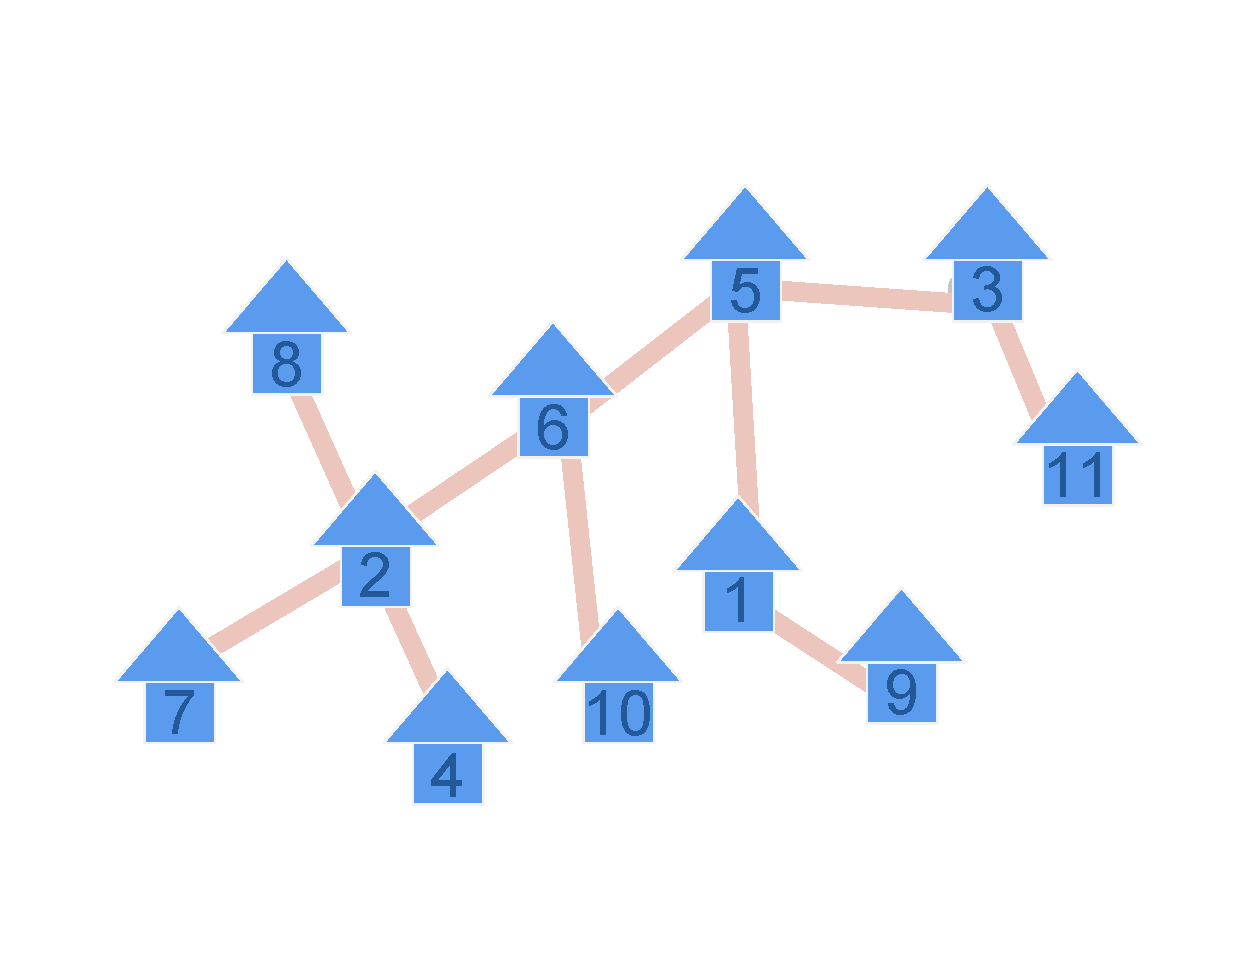
\includegraphics[scale=0.45]{../img/1_infinite_loop__cropped.pdf}
  \caption{\figtabsize {\residenceblock} street map.}
  \label{fig:streetmap}

  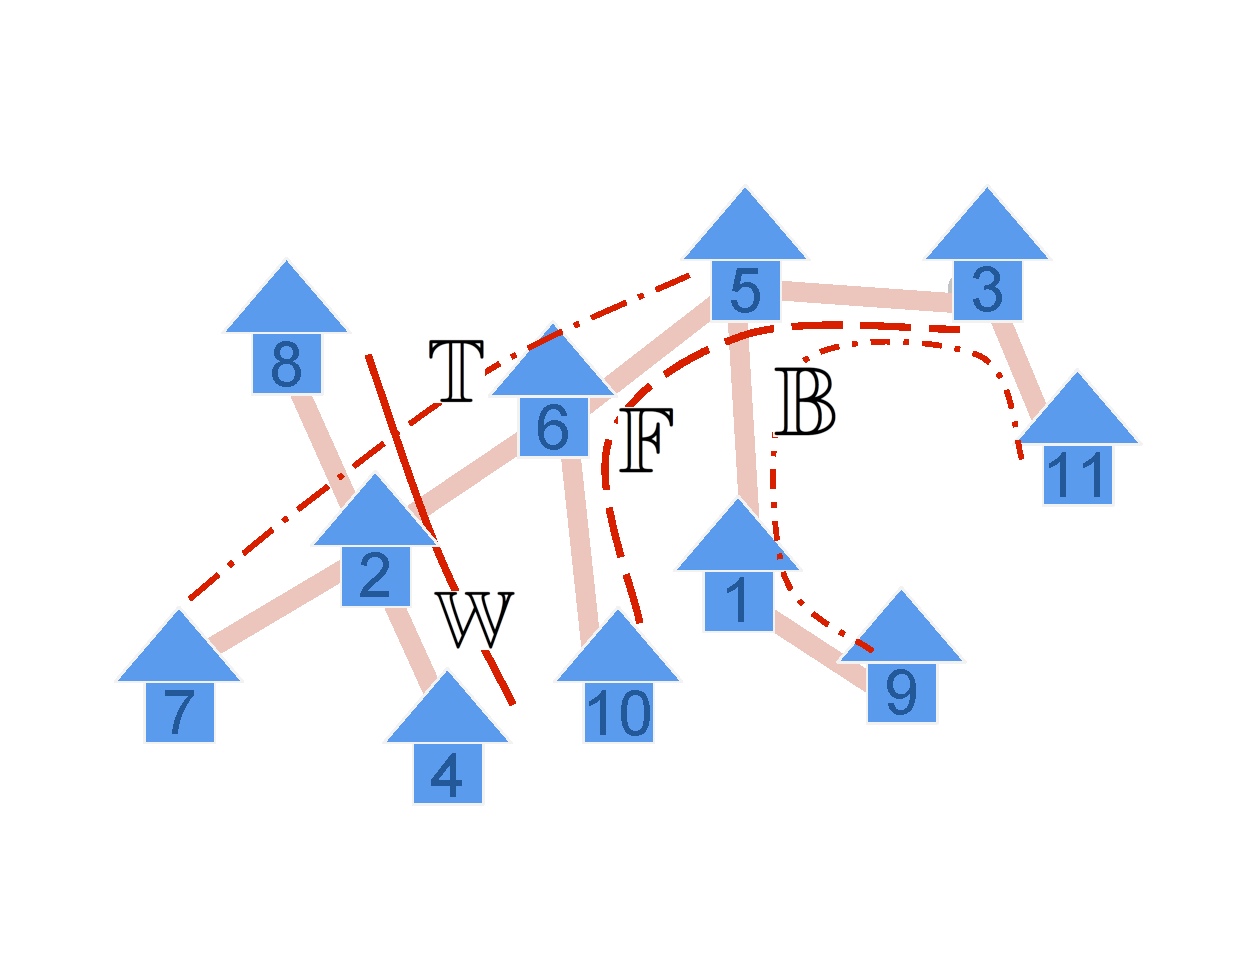
\includegraphics[scale=0.45]{../img/2_infinite_loop_BTWF__cropped.pdf}
  \caption[\figtabsize \residenceblock street map with study group
    routes allocated.]{\figtabsize {\residenceblock} street map with study group
    routes allocated. % Routes are color coded as follows: red for
%     \textcolor{red}{$\xLLL$} group, blue for \textcolor{blue}{$\xGGG$}
%     group, orange for \textcolor{yellow}{$\xBBB$} group, green for
%     \textcolor{green}{$\xTTT$} group
  }
  \label{fig:streetmappath}

  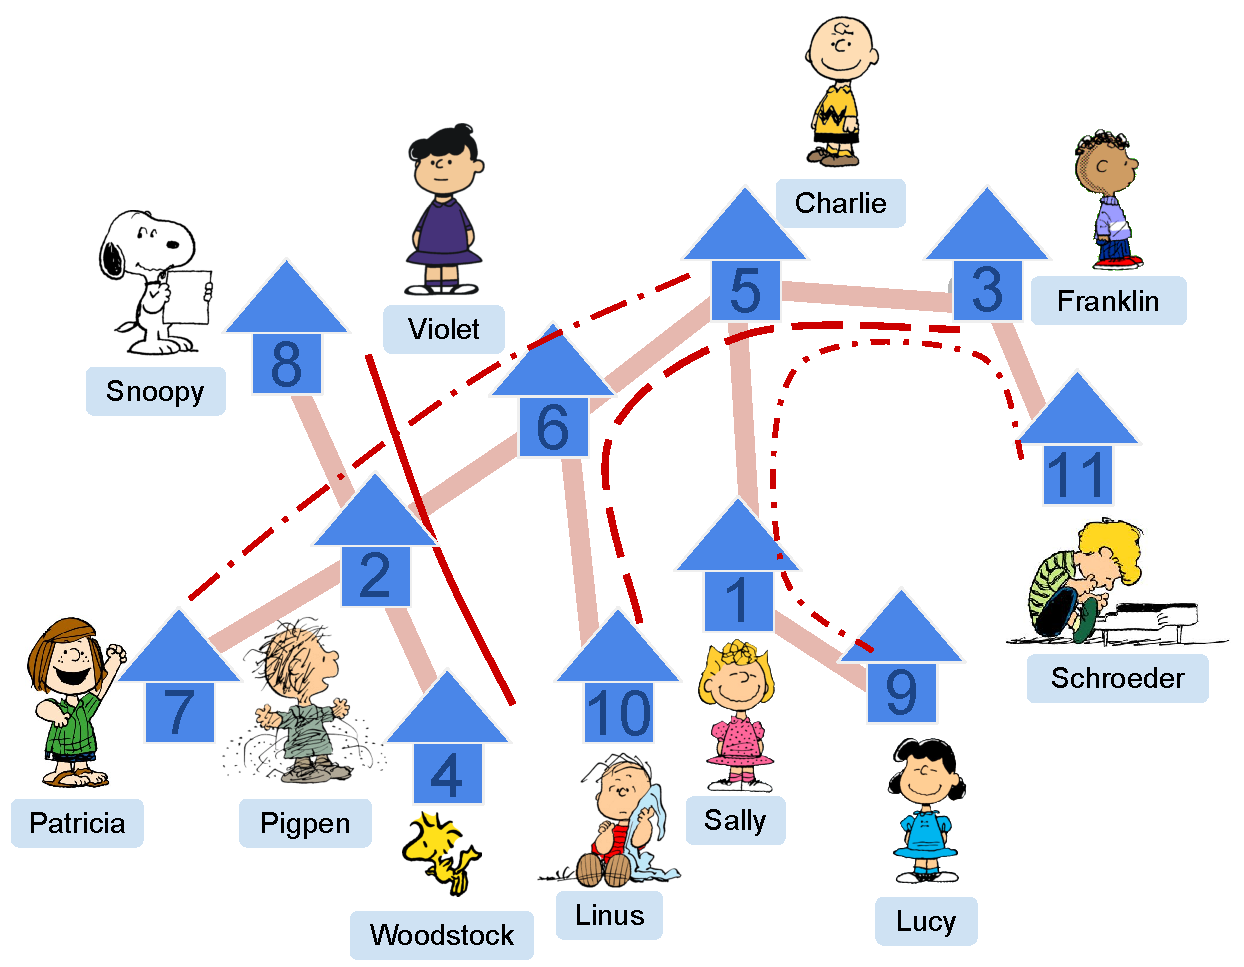
\includegraphics[scale=0.5]{../img/3_infinite_loop.pdf}
  \caption[\figtabsize Solution to the student accommodation
  problem.]{\figtabsize Individual allocation of apartments to
    students in {\residenceblock} that meets the requirements stated
    before.  % The routes are color coded as follows: red for
%     \textcolor{red}{$\xLLL$} group, blue for \textcolor{blue}{$\xGGG$}
%     group, orange for \textcolor{yellow}{$\xBBB$} group, green for
%     \textcolor{green}{$\xTTT$} group.
    \\ {\tiny {\em Peanuts images
        {\copyright} Charles Schulz}}}% YellowOrange
  \label{fig:streetmappathpeople}
\end{figure}

\subsection{Special case}
\label{sec:courseschedule}
As a special case of the study group accommodation problem, suppose
all the apartments are on the same street or if they are all lined up
on a single path, the street map becomes a tree that is just a
path. Then the problem becomes what is called an {\em interval
  assignment problem}. The idea of interval assignment may not be
obvious here; hence to see this, consider a different problem in
{\WSI} where the classes for these study groups courses need to be
scheduled during a day (or a week or any time period). Each study
group has a bunch of courses associated with it some of which may be
shared by two or more study groups. It is mandatory that a student who
is a member of a study group takes all the courses associated with
that group. There are slots during the day for classes to be held and
the problem is to allocate class slots to courses such that all the
classes of a study group are consecutive. % \footnote{It is debatable if this will
% not hamper the attention span and memory retention rate of the
% students but that is undoubtedly out of the scope of this
% thesis.}
The parallels between this class allocation problem and the
accommodation problem can be seen as follows. The set $U$ here, are
the courses offered (say Course 101 {\coneohone}, Course 102
{\coneohtwo} and so on). In this variation of the problem, the
collection $\cF$ is the set of study groups but the study groups are
filled by course IDs (in place of students in the earlier
example). For instance, Course 101 is mandatory for all study groups
$\xLLL$, $\xGGG$, $\xBBB$, $\xTTT$ and Course 102 is mandatory for
only the $\xLLL$ group) and so on. The sequence of class slots for the
day (or week or any time period) is analogous to the street map in the
accommodation problem. It is quite obvious now why this version of the
problem (where the ``target graph'' is a path and not any
tree) is called an interval assignment
problem.

The interval assignment problem to a set system is equivalent to the
consecutive-ones property (COP) problem in binary matrices\cite{wlh02,
  nsnrs09}.  The COP problem is to rearrange rows (columns) of a
binary matrix in such a way that every column (row) has its {\un}s
occur consecutively. If this is possible the matrix is said to have
the COP.  COP is a well researched combinatorial problem and has
several positive results on tests for it and computing the COP
permutation (i.e. the course schedule in the above illustration) which
will be surveyed later in this document. Hence we are interested in
extensions of COP, more specifically, the extension of interval
assignment problem to tree path assignment problem (which is
illustrated by the study group accommodation problem).


\section[Basic preliminaries]{Basic preliminaries} 
\label{sec:basicprelim}

Here we see some basic definitions and conventions necessary for the contents
of this thesis.

\subsection{Matrices}
If $n$ is a positive integer, $[n]$ denotes the set $\{1,2,... n\}$.

\begin{definition}[Binary matrix]
  \label{def:binmatrix}
  Let $M$ be an $n \times m$ matrix. $m_{i,j}$ denotes its $(i,j)$th
  element, i.e. element at $i$th row and $j$th column. $M$ is a
  \textbf{binary matrix} if each of its element is 0 or \un; for all
  $i \in [n]$ and $j \in [m]$, $m_{i,j} \in \{0, \un\}$
\end{definition}

\begin{definition}[Permutation]
  A \textbf{permutation} $\lambda$ of a set $X = \{x_1, x_2, \ldots
  x_n\}$ is a bijection $\lambda: X \rightarrow X$.  $\lambda$ may be
  written as a sequence $x_{i_1}x_{i_2}\ldots x_{i_n}$, where $i_j \in
  [n]$ to mean that $\lambda(x_j)= x_{i_j}$.  This document uses both
  notations as convenient in context.
\end{definition}

The idea of \cop of binary matrices was mentioned a few times in
earlier sections. Now we will see the formal definition of \COP in
Definition~\ref{{def:copmatrix}}.

\begin{definition}[\Cop (on columns)]
  \label{def:copmatrix}
  Let $M$ be a binary matrix.
  \begin{enumerate}
  \hangindent \defindent
  \item A \textbf{block of \un s (block of 0s)} in a column of $M$ is a maximal set of
    consecutive \un-entries (0-entries) in this column.
  \item $M$ has the \textbf{strong \cop
      (strong \COP)} if in every column the \un s appear consecutively,
    \ie if every column contains at most one block of \un s.
  \item $M$ has the \textbf{\cop} if its rows can be
    permuted in such a way that the resulting matrix has the strong \COP.
  \item If an ordering for the rows of $M$ gives the strong \COP, it
    is called a \textbf{\COP order} or \textbf{\COP permutation}.
  \end{enumerate}
\end{definition}

When the roles of rows and columns are exchanged in
Definition~\ref{def:copmatrix}, it defines \COP on rows. Both
are equivalent properties (for the purposes of this thesis) and both
conventions are seen the literature.
Figure~\ref{fig:cop-matrix} gives an example of \COP on columns.

\figcopmatrix

A less restrictive property of binary matrices that is a
generalization of the \COP is \crop (\CROP). The matrix can be
visualized to be wrapped around a horizontal cylinder and demands that
after some row permutations, if required, in every column the \un s
appear consecutively on the cylinder -- note that this implies the 0s
also appear consecutively.

\begin{definition}[\Crop (on columns)]
  \label{def:cropmatrix}
  Let $M$ be a binary matrix.
  \begin{enumerate}
  \hangindent \defindent
  \item $M$ has the \textbf{strong \crop (strong \CROP)} if in every
    column the \un s appear consecutively or the 0s appear
    consecutively or both.
  \item $M$ has the \textbf{\crop (\CROP)} if its rows can be permuted
    in such a way that the resulting matrix has the strong \CROP.
  \item If an ordering for the rows of $M$ gives the strong \CROP,
    then it is called the \textbf{\CROP ordering} or \textbf{\CROP
      permutation}.
  \end{enumerate}
\end{definition}

\subsection{Sets}

\begin{definition}[Set system]
  \label{def:setsystem}
  Let $U$ be a universe with $|U| = n$.  
  \begin{enumerate}
  \hangindent \defindent
  \item The set $\F \subseteq (2^{U} \setminus \emptyset)$ is called a
    \textbf{set system} with universe $U$.
  \item Two sets $S, S' \in \cF$ are said to \textbf{overlap}, denoted
    by $S \overlap S'$, if they have a non-empty intersection and
    neither is contained in the other.
    \[S \overlap S' \text{ \iff\ } S \cap S' \ne \emptyset, S
    \nsubseteq S', S' \nsubseteq S\]
  \end{enumerate}
\end{definition}


\begin{definition}
  \label{def:poset}    
%   Let $A$ be a set and $R$ be a binary relation $R \subseteq A \times
%   A$.

%   \textbf{poset}
  Let $X$ be a partially ordered set with $\preccurlyeq$ being the
  partial order on $X$.

  \begin{enumerate}
  \hangindent \defindent
%  \item \textbf{hasse diagram}
  \item An element $X_m \in X$ is a
    \textbf{maximal upper bound} of $X$ if $\nexists X_q \in X$ such
    that $X_m \preccurlyeq X_q$.  A maximal upper bound on $X$ is
    denoted by $mub(X)$.

  \item A set of sets form a \textbf{single
      inclusion chain} when the Hasse diagram of their subset relation
    forms a single chain.
  \end{enumerate}
\end{definition}

\subsection{Graphs}

\begin{definition}[Graph, Tree, Path]
  \label{def:graphtree}
  \begin{enumerate}
    \hangindent \defindent
  \item An \textbf{(undirected) graph} is $G = (V,E)$ is \stt $V$ is a
    finite set and $E$ is a set of ordered pairs, $E \subseteq V
    \times V$. An element in $V$ is called a \textbf{vertex
      (\emph{pl.} vertices)} and an element from $E$ is called an
    \textbf{edge}. $V$ and $E$ may be written as $V(G)$ and $E(G)$
    respectively. If $u,v \in V$ and $(u,v) \in E$ then $v$ is said to
    be \textbf{adjacent} to $u$ and vice versa. A \textbf{subgraph} of
    $G$ is a graph $G' = (V',E')$ \stt $V' \subseteq V$ and $E'
    \subseteq E$.

  \item A \textbf{path} is a graph $P = (V,E)$ with vertex set $V =
    \{v_1,\ldots,v_n\}$ and edge set $E= \{ (v_1,v_2),(v_2,v_3),
    \ldots,(v_{n-2},v_{n-1}),(v_{n-1},v_{n})\}$. The vertices $v_1,
    v_n$ are called the \textbf{endpoints} of $P$. The graph $P$ is
    called a \textbf{cycle} if it has an additional edge $(v_n,v_1)$.

  \item A \textbf{tree} is a graph $T$ that has no subgraph that is a
    cycle.
  \end{enumerate}
\end{definition}

% When refering to a tree as $T$ it could be a reference to the tree
% itself, or the vertices of the tree. This will be clear from the
% context.

\begin{definition}[Intersection graph]
  \label{def:intersectiongraph}
  Let $\cF$ be a set system. Then its \textbf{intersection graph}
  $\bI(\cF)$ is a graph \stt its vertex set has a bijection to $\cF$
  and there exists an edge between two vertices \iff their
  corresponding sets in $\cF$ have a non-empty intersection.
\end{definition}

\begin{definition}[Interval graph, Path graph]
  \label{def:pathgraph}
  Let $G$ be a graph.
  \begin{enumerate}
  \hangindent \defindent
  \item $G$ is an \textbf{interval graph} if there a set of intervals
    $\cI$ \stt $G$ is isomorphic to the intersection graph of
    $\cI$. \[G \cong \bI(\cI)\]
  \item $G$ is a \textbf{path graph} if there exists a (undirected
    unrooted) tree $T$ and a set of paths from $T$, $\cP$ \stt $G$ is
    isomorphic to the intersection graph of $\cP$. \[G \cong
    \bI(\cP)\] Path graphs are also known as \uvgraphs (Undirected
    tree where paths intersect in a Vertex) \cite{mw86}.
  \item $G$ is a \textbf{chordal graph} if it has no induced cycle of
    length greater than 3. Moreover, a \textbf{chordal graph} is
    characterized as an intersection graph of subtrees of a tree.
  \end{enumerate}
\end{definition}

The set of interval graphs is a subset of set of path graphs which is
a subset of set of chordal graphs. In fact, there is another class
between chordal graphs and path graphs called RDV-graphs (Rooted
Directed tree where paths intersect in a Vertex)  \cite{mw86} which is
defined exactly as a path graph except that the trees are rooted and
directed. 

\section[Brief Survey]{Consecutive-ones Property - a Brief Survey}
\label{sec:background}

In this section, a brief survey of the consecutive-ones problem and
its optimization problems is presented.


\subsection{Matrices with COP}
\label{sec:copmatrices}
As seen earlier, the interval assignment problem (illustrated as the
course scheduling problem in Section~\ref{sec:problem}), is a special
case of the problem we address in this thesis, namely the tree path
labeling problem (illustrated as the \illustrationproblem). The
interval assignment problem and COP problem are equivalent
problems. In this section we will see some of the results that exists
in the literature today towards solving the COP problem and
optimization problems surrounding it.

% \begin{figure}[t] %[htbp]
%   \centering

%   {\figtabsize
%     \begin{tabular}[h]{l|lcccl}
%       $M_1$: & $M_1'$: &&&& $M_2$:\\
%       &&&&&\\
%       \begin{tabular}[h]{llll}
%         $c_1$ & $c_2$ &$c_3$ &$c_4$\\
%         &&&\\
%         \un & 0   & \un & 0\\
%         0   & \un & 0   & \un \\
%         \un & 0   & 0   & \un
%       \end{tabular}
%       &
%       \begin{tabular}[h]{llll}
%         $c_3$ &$c_1$ &$c_4$& $c_2$\\
%         &&&\\
%         \un & \un & 0 & 0\\
%         0 & 0 & \un & \un \\
%         0 & \un & \un & 0
%       \end{tabular}
%       &&&&
%       \begin{tabular}[h]{llll}
%         $d_1$ & $d_2$ &$d_3$ &$d_4$\\
%         % &&&\\
%         &&&\\
%         \un & \un & 0 & 0\\
%         0 & \un & \un & 0 \\
%         0 & \un & 0 & \un 
%       \end{tabular}
%     \end{tabular}
%   }

%   \caption[\figtabsize Matrices with and without COP.]{\figtabsize
%     Matrices with and without COP. $M_1$ has COP because by permuting
%     its columns, $c_1$-$c_4$, one can obtain $M_1'$ where the {\un}s
%     in each row are consecutive. $M_2$, however, does not have COP
%     since no permutation of its columns, $d_1$-$d_4$, will arrange
%     {\un}s in each row consecutively \cite{d08phd}.}

%   \label{fig:cop-matrix}
% \end{figure}

Recall that a matrix with COP is one whose rows (columns) can be
rearranged so that the {\un}s in every column (row) are in consecutive
rows (columns). % Figure~\ref{fig:cop-matrix} shows examples of this
% property. 
COP in binary matrices has several practical applications
in diverse fields including scheduling \cite{hl06}, information
retrieval \cite{k77} and computational biology \cite{abh98}.  Further,
it is a tool in graph theory \cite{mcg04} for interval graph
recognition, characterization of Hamiltonian graphs, planarity testing
\cite{bl76} and in integer linear programming \cite{ht02,hl06}.


The obvious first questions after being introduced to the consecutive
ones property of binary matrices are if COP can be detected
efficiently in a binary matrix and if so, can the COP permutation of
the matrix also be computed efficiently?  Recognition of COP in a
binary matrix is polynomial time solvable and the first such algorithm
was given by \cite{fg65}.  A landmark result came a few years later
when \cite{at72} discovered the families of forbidden submatrices that
prevent a matrix from having COP and most, if not all, results that
came later were based on this discovery which connected COP in binary
matrices to convex bipartite graphs. In fact, the forbidden
submatrices came as a corollary to the discovery that convex bipartite
graphs are AT-free on at least one of the partitions in
\cite{at72}. The first linear time algorithm for COP testing (COT) was
invented by \cite{bl76} using a data structure called \PQtrees.  Since
then several COT algorithms have been invented -- some of which
involved variations of \PQtrees \cite{mm96,wlh01,mcc04}, some involved
set theory and ICPIA \cite{wlh02,nsnrs09}, parallel COT
algorithms\cite{as95,bs03,ly91} and certifying algorithms\cite{mcc04}.

The construction of \PQtrees in \cite{bl76} draws on the close
relationship of matrices with \COP to interval graphs. A PQ tree of a
matrix is one that stores all row (column) permutations of the matrix
that give the COP orders (there could be multiple orders of rows or
columns) of the matrix. This is constructed using an elaborate linear
time procedure and is also a test for planarity.  PQR trees is a
generalized data structure based on PQ trees \cite{mm96,mpt98}.
\cite{tm05} describes an improved algorithm to build PQR
trees. \cite{wlh02} describes the simpler algorithm for COT. Hsu also
invented PC trees \cite{wlh01} which is claimed to be much easier to
implement. \cite{nsnrs09} describes a characterization of
consecutive-ones property solely based on the cardinality properties
of the set representations of the columns (rows); every column (row)
is equivalent to a set that has the row (column) indices of the rows
(columns) that have one entries in this column (row). This is
interesting and relevant, especially to this thesis because it
simplifies COT to a great degree.

\cite{mcc04} describes a different approach to COT. While all previous
COT algorithms gave the COP order if the matrix has the property but
exited stating negative if otherwise, this algorithm gives an evidence
by way of a certificate of matrix even when it has no COP. This
enables a user to verify the algorithm's result even when the answer
is negative. This is significant from an implementation perspective
because automated program verification is hard and manual verification
is more viable. Hence having a certificate reinforces an
implementation's credibility. Note that when the matrix {\em has} COP,
the COP order is the certificate.  The internal machinery of this
algorithm is related to the weighted betweenness problem
addressed in \cite{co98}.  

\subsection{Optimization problems in COP}
\label{sec:optcop}

So far we have been concerned about matrices that have the consecutive
ones property. However in real life applications, it is rare that data
sets represented by binary matrices have COP, primarily due to the
noisy nature of data available. At the same time, COP is not arbitrary
and is a desirable property in practical data representation
\cite{co98,jkckv04,k77}. In this context, there are several
interesting problems when a matrix does not have COP but is ``close''
to having COP or is allowed to be altered to have COP. These are the
optimization problems related to a matrix which does not have
COP. Some of the significant problems are surveyed in this section.

\cite{at72} showed that a matrix that does not have COP have certain
substructures that prevent it from having COP. Tucker classified these
forbidden substructures into five classes of submatrices. This result
is presented in the context of convex bipartite graphs which
\cite{at72} proved to be AT-free in one of the partitions. By
definition, convex bipartite graph have half adjacency matrices that
have COP on either rows or columns (graph is biconvex if it has COP on
both)\cite{d08phd}. A half adjacency matrix is a binary matrix
representing a bipartite graph as follows. The set of rows and the set
of columns form the two partitions of the graph. Each row node is
adjacent to those nodes that represent the columns that have {\un}s in
the corresponding row. \cite{at72} proves that this bipartite graph
has no asteroidal triple in vertex partition corresponding to rows if
and only if the matrix has COP on columns and goes on to identify the
forbidden substructures for these bipartite graphs. The matrices
corresponding to these substructures are the forbidden submatrices.

Once a matrix has been detected to not have COP (using any of the COT
algorithms mentioned earlier), it is naturally of interest to find out
the smallest forbidden substructure (in terms of number of rows and/or
columns and/or number of entries that are {\un}s). \cite{d08phd}
discusses a couple of algorithms which are efficient if the number of
{\un}s in a row is small. This is of significance in the case of
sparse matrices where this number is much lesser than the number of
columns. $(*,\Delta)${\em -matrices} are matrices with no restriction
on number of {\un}s in any column but have at most $\Delta$ {\un}s in
any row. {\sc Min COS-R (Min COS-C), Max COS-R (Max COS-C)} are
similar problems which deals with inducing COP on a matrix. In {\sc
  Min COS-R (Min COS-C)} the question is to find the minimum number of
rows (columns) that must be deleted to result in a matrix with COP.
In the dual problem {\sc Max COS-R (Max COS-C)} the search is for the
maximum number of rows (columns) that induces a submatrix with
COP. Given a matrix $M$ with no COP, \cite{b75-phd} shows that finding
a submatrix $M'$ with all columns but a maximum cardinality
subset of rows such that $M'$ has COP is NP complete. \cite{hg02}
corrects an error of the abridged proof of this reduction as given in
\cite{gj79}.  \cite{d08phd} discusses all these problems in detail
giving an extensive survey of the previously existing results which
are almost exhaustively all approximation results and hardness
results. Taking this further, \cite{d08phd} presents new results in
the area of parameterized algorithms for this
problem.

Another problem is to find the minimum number of entries in the matrix
that can be toggled to result in a matrix with COP.  \cite{v85}
discusses approximation of {\sc COP Augmentation} which is the problem
of changing of the minimum number of zero entries to {\un}s so that
the resulting matrix has COP. As mentioned earlier, this problem is
known to be NP complete due to \cite{b75-phd}. \cite{v85} also proves,
using a reduction to the longest path problem, that finding a Tucker's
forbidden submatrix of at least $k$ rows is NP complete.

\cite{jkckv04} discusses the use of matrices with almost-COP (instead
of one block of consecutive {\un}s, they have $x$ blocks, or {\em
  runs}, of consecutive {\un}s and $x$ is not too large) in the
storage of very large databases.  The problem is that of reordering of
a binary matrix such that the resulting matrix has at most $k$ runs of
{\un}s. This is proved to be NP hard using a reduction from the
Hamiltonian path problem.


% \section[Some applications of \COP]{Application of COP in Areas of Graph Theory and
%   Algorithms}
% \label{sec:appcopGTA}

% \temptext{Combine COP in Relational Database Model + COP in Graph
%   Isomorphism + Certifying Algorithms}

% %\subsection{COP in Relational Database Model}
% \label{sec:apprdbm}
% \tnote{(set systems theme)}

% %\subsection{}
% \label{sec:appgraphiso}
% \tnote{(canonization theme)}

% %\subsection{}
% \label{sec:appcertalgo}
% \tnote{ (certification McC04 theme)}


\section[Generalization of COP]{Generalization of COP - the Motivation}
\label{sec:motive}
Section~\ref{sec:copmatrices} introduced a succinct characterization
for consecutive-ones property which is solely based on the cardinality
properties of the set representations of the matrix's columns
\cite{nsnrs09}. This result is very relevant to this thesis because
aside from it simplifying COT to a great degree, our generalization
problem is motivated by their results.

\cite{nsnrs09} characterizes interval assignments to the sets which
can be obtained from a single permutation of the rows.  For an
assignment to be feasible, the cardinality of the interval assigned to
each set in the system must be same as the cardinality of the set, and
the intersection cardinality of any two intervals must be same as the
intersection cardinality of their corresponding sets.  While this is
obviously a necessary condition, this result shows this is also
sufficient.  \cite{nsnrs09} calls this an Intersection Cardinality
Preserving Interval Assignment (ICPIA).  This paper generalizes the
idea from \cite{wlh02} of decomposing a given binary matrix into prime
matrices for COT and describes an algorithm to test if an ICPIA exists
for a given set system.

The equivalence of the problem of testing for the consecutive-ones
property to the constraint statisfaction problem of interval
assignment \cite{nsnrs09} or interval labeling \cite{kklv10} is as
follows. Every column (row) of the binary matrix can be converted into
a set of non-negative integers which are the indices of rows (columns)
with {\un}s in that column (row). It is apparent that if the matrix
has COP in columns (rows), then constructing such sets after applying
the COP permutation to the rows (columns) of the matrix will result in
sets with consecutive integers. In other words, after application of
COP reordering, the sets are intervals. Indeed the problem now becomes
finding interval assignments to a given set system such that there
exists a permutation of the universe of set of row indices (column
indices) which converts each set to its assigned interval.

The problem of interest in this thesis, namely, tree path labeling
problem, is a natural generalization of the interval assignment
problem or the COT problem. The problem is defined as follows -- given
a set system $\cF$ from a universe $U$ and a target tree $T$, does
there exist a bijection from $U$ to the vertices of $T$ such that each
set in the system maps to a path in $T$.  We refer to this as the
{\CFTPL} problem or simply {\em tree path labeling} problem for an
input set system and target tree pair -- $(\cF,T)$. The special case
of the target tree being a path, is the interval assignment problem.
We focus on generalizing the notion of an ICPIA \cite{nsnrs09} to
characterize feasible path assignments.  We show that for a given set
system $\cF$, a tree $T$, and an assignment of paths from $T$ to the
sets, there is a feasible\footnote{The notion of {\em feasibility} is
  formally defined in Section~\ref{ch:prelims}.}  bijection between
$U$ and $V(T)$ if and only if the intersection cardinalities among any
three sets (not necessarily distinct) is equal to that of the
corresponding paths assigned to them and the input passes a filtering
algorithm (described in this paper) successfully.  This algorithmic
characterization gives a natural data structure that stores all the
\remove{relevant} feasible bijections between $U$ and $V(T)$. This
reduces the search space for the solution considerably from the
universe of all possible bijections between $U$ and $V(T)$ to only
those bijections that maintain the characterization.  Further, the
filtering algorithm is also an efficient algorithm to test if a tree
path labeling\footnote{The terms {\em tree path labeling} and {\em
    tree path assignment} are, in informal language,
  synonyms. Formally, the former refers to the bijection $\cl: \cF
  \rightarrow \cP$. The latter refers to the set of ordered pairs
  $\{(S, P) \mid S \in \cF, P \in \cP\}$. $\cP$ is a set of paths on
  $T$.} is feasible.


\section[Summary of new results]{Summary of New Results in this Thesis}
\label{sec:results}

We see in Section~\ref{sec:motive} that pairwise intersection
cardinality preservation is necessary and sufficient for an interval
assignment to be feasible for a given hypergraph\footnote{A {\em
    hypergraph} is an alternate representation of a set system and
  will be used in this thesis.}~\footnote{See Section~\ref{ch:prelims}
  for the formal definition.} and thus is a characterization for COP
\cite{nsnrs09}. In our work we extend this characterization and find
that trio-wise intersection cardinality preservation makes a tree path
labeling\footnote{A {\em tree path labeling} $\cl$ is a bijection of
  paths from the target tree $T$ to the hyperedges in given hypergraph
  $\cF$.}~\footnotemark[4] (TPL) feasible, which is a generalization
of the COP problem. This problem is defined by \FTPL (See
Section~\ref{sec:myresearchintro} for problem definition). %as follows.

% {\small
%   \begin{minipage}[h]{5in}
%     % \begin{singlespace}
%     \vspace{2mm}
%     {\large \FTPL}\\
%     \begin{tabular}[t]{l|l}
%       \hline\\
%       {\tt Input} & 
%       \begin{minipage}[t]{\probdefwidth}
%         A hypergraph $\cF$ with vertex set $U$, a tree $T$, a set of
%         paths $\cP$ from $T$ and a
%         bijection $\cl$~$:$~$\cF \rightarrow \cP$.\\
%       \end{minipage}\\
%       {\tt Question} &
%       \begin{minipage}[t]{\probdefwidth}
%         Does there exist a bijection $\phi$~$:$~$U \rightarrow V(T)$
%         such that $\phi$ when applied on any hyperedge in $\cF$ will
%         give
%         the path mapped to it by the given tree path labeling $\cl$.\\
%         { i.e., $\cl(S) = \{\phi(x) \mid x \in S\}$, for every
%           hyperedge $S \in \cF$.}
%       \end{minipage}\\
%     \end{tabular}
%     % \end{singlespace}
%   \end{minipage}\\
% }

We give a necessary and sufficient condition by way of {\em
  Intersection Cardinality Preservation Path Labeling} (ICPPL) and a
filtering algorithm for {\FTPL} to output in affirmative. ICPPL
captures the trio-wise cardinality property described
earlier\footnote{See Section~\ref{sec:feasible} for the definition of
  ICPPL.}. This characterization can be checked in polynomial time.  A
relevant consequence of this constructive procedure is that it is
sufficient to iteratively check if three-way intersection
cardinalities are preserved.  In other words, in each iteration, it is
sufficient to check if the intersection of any three hyperedges is of
the same cardinality as the intersection of the corresponding paths.
Thus this generalizes the well studied question of the feasible
interval assignment problem which is the special case when the target
tree $T$ is simply a path \cite{wlh02,nsnrs09}.

Aside from checking if a given TPL is feasible, we also solve the
problem of computing a feasible TPL for a given hypergraph and target
tree, if one exists. This problem is the {\CFTPL} problem (See
Section~\ref{sec:myresearchintro} for problem definition). %, is defined as follows.

% {\small
%   \begin{minipage}[h]{5in}
%     % \begin{singlespace}
%     \vspace{2mm}
%     {\large \CFTPL}\\
%     \begin{tabular}[t]{l|l}
%       \hline\\
%       {\tt Input} & 
%       \begin{minipage}[t]{\probdefwidth}
%         A hypergraph $\cF$ with vertex set $U$ and a tree $T$.\\
%       \end{minipage}\\

%       {\tt Question} &
%       \begin{minipage}[t]{\probdefwidth}
%         Does there exist a set of paths $\cP$ from $T$ and a bijection
%         $\cl$~$:$~$\cF \rightarrow \cP$, such that {\FTPL} returns
%         {\bf true} on $(\cF, T, \cl)$.
%       \end{minipage}\\
%     \end{tabular}
%     % \end{singlespace}
%   \end{minipage}\\
% }

We present a polynomial time algorithm for {\CFTPL} when the target
tree $T$ belongs to a special class of trees called {\em \kstars} and
when the hyperedges in the hypergraph $\cF$ have at most $k+2$
vertices (\CFTPLKTREE -- See Section~\ref{sec:myresearchintro} for
problem definition). A couple of examples of {\kstars} are given in
Figure~\ref{fig:ksubstar}.


\begin{figure}[t]
  \centering
  \begin{tabular}[h]{ccccc}
    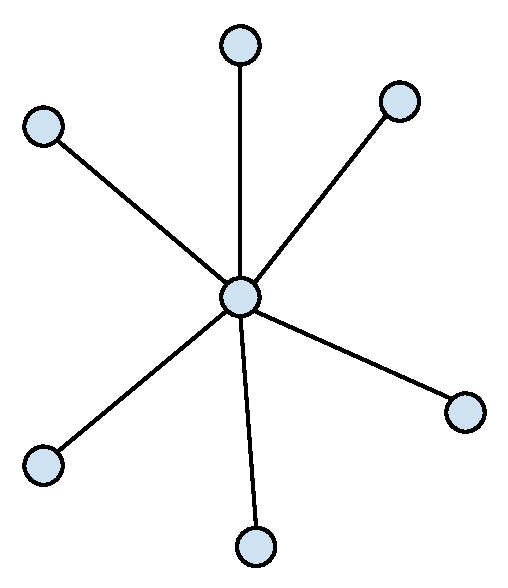
\includegraphics[scale=0.3]{../img/star.pdf} &&&&
    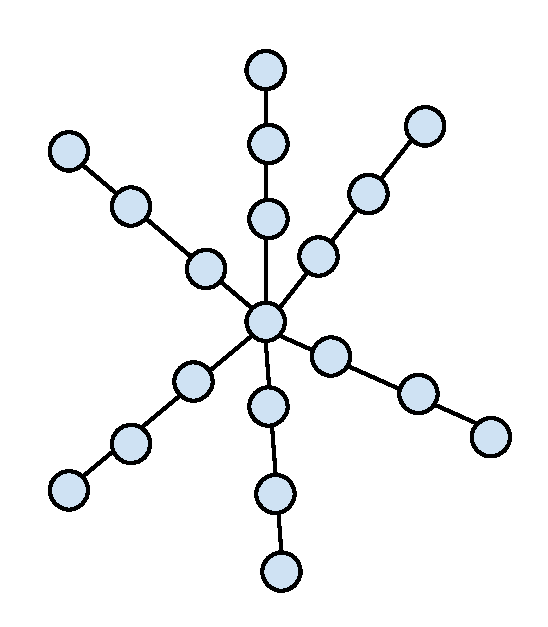
\includegraphics[scale=0.3]{../img/kstar.pdf}\\
    (a) &&&& (b)
  \end{tabular}
  \caption{\figtabsize Examples of {\kstars}. (a) $k = 0$ (b) $k = 2$
  }
  \label{fig:ksubstar}
\end{figure}

% {\small
%   \begin{minipage}[h]{5in}
%     % \begin{singlespace}
%     \vspace{2mm}
%     {\large \CFTPLKTREE}\\
%     \begin{tabular}[t]{l|l}
%       \hline\\
%       {\tt Input} & 
%       \begin{minipage}[t]{\probdefwidth}
%         A hypergraph $\cF$ with vertex set $U$ such that every
%         hyperedge
%         $S \in \cF$ is of cardinality at most $k+2$ and a {\kstar} $T$.\\
%       \end{minipage}\\
%       {\tt Question} &
%       \begin{minipage}[t]{\probdefwidth}
%         Does there exist a set of paths $\cP$ from $T$ and a bijection
%         $\cl$~$:$~$\cF \rightarrow \cP$, such that {\FTPL} returns
%         {\bf true} on $(\cF, T, \cl)$.
%       \end{minipage}\\
%     \end{tabular}
%     % \end{singlespace}
%   \end{minipage}\\
% }

In spite of this being a restricted case, we believe that our results
are of significant interest in understanding the nature of {\sc Graph
  Isomorphism} which is polynomial time solvable in interval graphs
while being hard on path graphs\cite{kklv10}. {\kstars} are a class of
trees which are in many ways very close to intervals or paths. Each
ray\footnote{The path from a leaf to the root, the vertex with highest
  degree, is called a {\em ray} of the \kstar.}~\footnotemark[4] are
independent except for the root\footnote{The vertex with maximum
  degree in a {\kstar} is called {\em root}.}~\footnotemark[4] and
hence can be considered as an independent interval till the root. Our
algorithm builds on this fact and uses the interval assignment
algorithm\cite{nsnrs09} up until ``reaching'' the root and then uses
the trio-wise intersection cardinality (the extra condition in ICPPL
that generalizes ICPIA) check to resolve the ambiguity about which ray
the algorithm should ``grow'' the solution into in the next iteration.

We also have an algorithm for solving {\CFTPL} with no restrictions on
the target tree or set size which runs in exponential time.  This
algorithm finds a path labeling from $T$ by decomposing the problem
into subproblems of finding path labeling of subsets of $\cF$ from
subtrees of $T$. Given the fact that binary matrices naturally
represent a set system (see Section~\ref{sec:motive}) and that the
{\em overlap} relation between the sets involved is an obvious
equivalence relation, $\cF$ quite naturally partitions into
equivalence classes known as {\em overlap components}. In the context
of COP, overlap components were used in \cite{wlh02} and
\cite{kklv10}. Moreover, \cite{nsnrs09} discovered that these
equivalence classes form a total order. We extend this to TPL and find
that when $\cF$ is a path hypergraph\footnote{If there exists an FTPL
  for a hypergraph $\cF$, it is called a path hypergraph.}, the
classes can be partially ordered as an in-tree in polynomial
time. Once $\cF$ is ``broken'' into overlap components, one must
identify the subtree of $T$ that it needs to map to and this is the
hard part which is currently open to be solved in polynomial time.

\setcounter{endnote}{0} % need to empty the file too. how?!
\xclearpage


%\chapter{\CoP\,-- A Survey of Important Results}
\chapter[COP -- A Survey]{Consecutive-ones Property -- A Survey of
  Important Results}
\label{ch:copsurvey}

This chapter surveys several results that are significant to this
thesis or to \COP in general. These predominantly pertain to
characterizations of \COP, algorithmic tests to check for \COP,
optimization problems on binary matrices that do not have \COP and
some applications of \COP.


The chapter is organized as follows. Section~\ref{sec:copgraphtheory}
discusses the close connections of matrices with \COP in graph
theory. Section~\ref{sec:surveycoptest} discusses the important
results in the area of \cop testing (COT) -- we describe the history
of this problem's several solutions including Tucker's forbidden
submatrices, \PQtree, \PQRtree and ICPIA. 

It is worth noting that we make a very interesting observation about
\PQRtree, generalised \PQtree and \gPQtree\ -- that the theory that
all these independent data structures are built upon are very similar
and equivalent. This is exhaustively described in
Section~\ref{sec:surveycertalgo} and curiously, this comparison has
not been encountered by us in the literature.

Section~\ref{sec:surveycopopt} briefly touches upon the scenario of
algorithmically verifying that a matrix indeed does not have \COP. Its
significance lies in the fact that almost all \COT algorithms, upon
detection of no \COP, simply reports the same without any certificate
for verification during algorithm implementation. The two approaches
presented in this section gives a certificate.


\section{\COP in Graph Theory}
\label{sec:copgraphtheory}

\COP is closely connected to several types of graphs by way of
describing certain combinatorial graph properties. There are also
certain graphs, like convex bipartite graphs, that are defined solely
by one of its associated matrix having \COP.  In this section we will
see the relevance of \cop to graphs.  To see this we introduce certain
binary matrices that are used to define graphs in different
ways. While adjacency matrix is perhaps the most commonly used such
matrix, Definition~\ref{def:graphmatrices} defines this and a few
more.

\begin{definition}
  {\em Matrices that define graphs. \cite[Def.~2.4]{d08phd}.}  
  \label{def:graphmatrices} 
  Let $G$ and $H$ be defined as follows. $G = (V,E_G)$ is a graph with
  vertex set $V = \{v_i \mid i \in [n]\}$ and edge set $E_G \subseteq
  \{(v_i,v_j) \mid i, j \in [n]\}$ such that $|E_G| = m$. $H = (A, B,
  E_H)$ is a bipartite graph with partitions $A = \{a_i \mid i \in
  [n_a]\}$ and $B = \{b_i \mid i \in [n_b]\}$.
  \begin{enumerate}[{\ref{def:graphmatrices}}--i.]
  \item \emph{Adjacency matrix} of $G$ is the symmetric $n \times n$
    binary matrix $M$ with $m_{i,j} = \un$ \iff $(v_i,v_j) \in E_G$
    for all $i,j \in [n]$.
  \item \emph{Augmented adjacency matrix} of $G$ is obtained from its
    adjacency matrix by setting all main diagonal elements to \un, \ie
    $m_{i,i} = \un$ for all $i \in [n]$.
  \item \emph{Maximal clique matrix} or \emph{vertex-clique incidence
      matrix} of $G$ is the $n \times k$ binary matrix $M$ with
    $m_{i,j} = \un$ \iff $v_i \in C_j$ for all $i \in [n], j \in [k]$
    where $\{C_j \mid j \in [k]\}$ is the set of maximal cliques of
    $G$.
    \label{def::maxcliquematrix}
  \item \emph{Half adjacency matrix} of $H$ is the $n_a \times n_b$
    binary matrix $M$ with $m_{i,j} = \un$ \iff $(a_i, b_j) \in E_H$.
  \end{enumerate}
\end{definition}

\figgraphmatrices

Now we will see in Definition~\ref{def:graphwithcop} certain graph
classes that is related to \COP or \CROP.\\

\begin{definition}{\emph{Graphs that relate to
      COP.\cite[Def.~2.5]{d08phd}}} %
  \label{def:graphwithcop} %
  Let $G$ be a graph and $H$ be a bipartite graph.
  \begin{enumerate}[\ref{def:graphwithcop}--i.]
  \item $G$ is \emph{convex-round} if its adjacency matrix has the
    \CROP.
  \item \label{def::concave-round} $G$ is \emph{concave-round} if its
    augmented adjacency matrix has \CROP. \cite{bhy00}
  \item $G$ is an \emph{interval graph} if its vertices can be mapped
    to intervals on the real line \stt two vertices are adjacent \iff
    their corresponding intervals overlap \cite{sb59}.  $G$ is an interval graph \iff its maximal clique matrix
    has COP \cite{fg65} (This follows \cite{gh64} which states
      that the maximal cliques of interval graph $G$ can be linearly
      ordered \stt for all $v \in V(G)$, cliques containing $v$ are
      consecutive in the ordering \cite[Th. 8.1]{mcg04}.)
    \begin{enumerate}[a.]
    \item $G$ is a \emph{unit interval graph} if it is an interval
      graph \stt all intervals have the same length.
    \item $G$ is a \emph{proper interval graph} if it is an interval
      graph \stt no interval properly contains another.
    \end{enumerate}
    The set of unit interval graphs and the set of proper interval
    graphs coincide \cite{rob69, gar07}.
 \item $G$ is a \emph{circular-arc graph} if its vertices can be
    mapped to a set of arcs on a circle \stt two vertices are adjacent
    \iff their corresponding arcs overlap.
  \item $H$ is \emph{convex bipartite on columns (rows)} if its half
    adjacency matrix has \COP on rows (columns).%
    \label{def::convexbi}
  \item $H$ is \emph{biconvex bipartite} or \emph{doubly
      convex}\cite{yc95} if its half adjacency matrix has \COP on both
    rows and columns.
  \item $H$ is \emph{circular convex} if its half adjacency matrix has
    \CROP.
  \end{enumerate}
\end{definition}

Interval graphs\footnote{\cite{mcc04} cites that the problem of
  recognizing interval graphs has significance in molecular
  biology. Interestingly, in the late 1950s, before the structure of
  DNA was well-understood, Seymour Benzer was able to show that the
  intersection graph of a large number of fragments of genetic
  material was an interval graph \cite{sb59}. This was regarded as
  compelling evidence that genetic information was somehow arranged
  inside a structure that had a linear topology which we now know to
  be true from the discovery of linear structure of DNA.}and
circular-arc graphs have a long history in research.  The interest
around them is due to their very desirable property that several
problems that are NP-complete on general graphs, like finding a
maximum clique or minimum coloring or independent set, are polynomial
time solvable in these graph classes \cite{clrs01}.  In a similar
fashion, a lot of problems that are hard on general matrices have
efficient solutions on matrices with \COP or \CROP \cite[more
citations pg.\,33]{d08phd}.

Table~\ref{tab:graphmatrices} summarises the way these graphs are
characterized by their matrices having \COP or \CROP.
Our focus in this chapter (and thesis) is mainly \COP and 
having seen how useful \COP is in identifying or characterizing many
types of graphs, we will now see results that study recognition of \COP
in matrices in the following section.

\tabgraphmatrices  

\section{Matrices with COP}
\label{sec:surveycoptest}

The most important questions with respect to a particular 
property desired in a structure/object are perhaps the following.
\begin{itemize}%[]
\singlespacing
\item Does the desired property exist in the given input?
\item If the test is affirmative, what is a certificate of the affirmative?
\item If the test is negative, what are the optimization possibilities
  for the property in the input? In other words, how close to having the
  property can the input be?
\item If the test is negative, what is a certificate of the negative?
\end{itemize}

In this section and the rest of the chapter we see results that shaped the
correponding areas respectively for \cop in binary matrices.

\begin{enumerate}[a.]
\singlespacing
\item \label{q:testcop} Does a given binary matrix have \COP?
\item \label{q:copperm} What is the \COP permutation for the given matrix with \COP?
\item \label{q:copopt} What are the optimizations possible and practically useful on
  the given matrix without \COP?
\item \label{q:nocopcert} If algorithm for (\ref{q:testcop}) returns
  \textbf{false}, can a certificate for this be computed?
\end{enumerate}

Without doubt, besides computing answers to these questions, we are
interested in the efficiency of these computations in terms of
computational complexity theory. Results towards
questions~(\ref{q:testcop}) and (\ref{q:copperm}) are surveyed in this
section. Those for question~(\ref{q:copopt}) are discussed in
Section~\ref{sec:surveycopopt} and question~(\ref{q:nocopcert}) is discussed
in Section~\ref{sec:surveycertalgo}.

It may be noted that one way to design an algorithm to test for \COP
is by deriving one from any interval graph recognition algorithm using
the result \cite{hmpv00} \cite[Th~2.7]{d08phd} which demonstrates how
such a derivation can be done.  They use something called {\em Lex-BFS
  ordering} of the vertices of a graph to decide in linear time
whether the graph is an interval graph. They also show how any
interval graph recognition algorithm can be used to recognize matrices
with \COP. This is shown in Theorem~\ref{th:intgraphcop}.

\begin{theoremsansproof}[{\cite[Th.~2]{hmpv00}}]
  \label{th:intgraphcop}
  For a binary matrix $M$ the following statements are equivalent.
  \begin{enumerate}
  \item The row adjacency graph $G_r(M)$ is an interval graph and $M$
    is its maximal clique matrix.
  \item The columns of $M$ are maximal and $M$ has the \COP for rows.
  \end{enumerate}
\end{theoremsansproof}


However, this does not necessarily yield an efficient algorithm. We
will see results that directly solve the problem on matrices since it
is known that questions~(\ref{q:testcop}) and (\ref{q:copperm}) stated
above for \COP are efficiently solvable.  Table~\ref{tab:cophistory}
gives a snapshot of these results.



\tabcophistory

The first polynomial time algorithm for \COP testing was by
\cite{fg65} which uses overlapping properties of columns with \un
s. Their result has close relations to the characterization of
interval graphs by \cite{gh64}. A graph $G$ is an interval graph \iff
all its maximal cliques can be linearly ordered \stt for any vertex
$v$ in $G$, all the cliques that $v$ is incident on are consecutive in
this order. Clearly, this means that the maximal clique incidence
matrix (see
Definition~\ref{def:graphmatrices}~\ref{def::maxcliquematrix}) must
have \COP on rows.

A few years later, a deeply significant result based on very different
ideas in understanding \COP came from Tucker which gave a
combinatorial (negative) characterization of matrices with COP
\cite{at72}. This result influenced most of the \COP results that
followed in the literature including linear time algorithms for \COP
recognition.


\subsection{Tucker's forbidden submatrices for \COP}
\label{sec:tucker}

\cite{at72} discovered certain forbidden structures for convex
bipartite graphs\footnote{The terminology in \cite{at72} differs. It
  uses the term {\em graphs with $V_1$-consecutive arragement} instead
  of {\em convex bipartite graphs}.} and by definition of this graph
class, this translates to a set of forbidden submatrices for matrices
with \cop.  The following are the theorems from \cite{at72} that
acheived this characterization.


Theorem~\ref{th:tuckeratfree} states that convex bipartite graphs
cannot have {\em asteroidal triples} (see
Definition~\ref{def:asteroidal}) contained in the corresponding vertex
partition. This partition of the bipartite graph corresponds to
columns (rows) if its half adjacency matrix has \COP columns (rows).
Theorem~\ref{th:tuckerforbidden} lists the structures in a bipartite
graph that force one of its vertex partitions to have asteriodal
triples -- in other words, it identifies the subgraphs that prevent
the graph from being convex bipartite.

\begin{definition}[Asteroidal triple]
  \label{def:asteroidal}
  % If $G = (V,E)$ is a graph, a set of three vertices from $V$ form
  % an {\em asteroidal triple} if between any two of them there exists
  % a path in $G$ that does not contain any vertex from the closed
  % neighborhood of the third vertex.
  An {\em asteroidal triple} in a graph $G$ is a tuple of vertices
  $\{v_1,v_2,v_3\} \subset V$ such that between every pair of vertices
  from this tuple there exists a path that avoids the closed
  neighbourbood of the third vertex.
\end{definition}

\begin{theoremsansproof}
  [{\cite[Th.~6]{at72}, \cite[Th.~2.3]{d08phd}}]%\\
  A bipartite graph $G = (V_1, V_2, E)$ is convex bipartite on
  columns\footnote{Abridged to match terminology adopted in this
    document. See previous note.} \iff $V_1$ contains no asteroidal
  triple of $G$.
  \label{th:tuckeratfree}
\end{theoremsansproof}

\begin{theoremsansproof}
  [{\cite[Th.~7]{at72}, \cite[Th.~2.4]{d08phd}}]%\\
  In a bipartite graph $G = (V_1, V_2, E)$ the vertex set $V_1$
  contains no asteroidal triple \iff $G$ contains none of the graphs
  $G_{I_k}$, $G_{II_k}$, $G_{III_k}$ (with $k \ge 1$), $G_{IV}$,
  $G_{V}$ as shown in Figure~\ref{fig:forbiddensubgraphs} as subgraphs.
  \label{th:tuckerforbidden}
\end{theoremsansproof}


\figforbiddensubgraphs


Theorem~\ref{th:tuckeratfree} and Theorem~\ref{th:tuckerforbidden}
result in the following Theorem~\ref{th:tuckercop} which characterizes
matrices with \COP.

\begin{theoremsansproof}
  [{\cite[Th.~9]{at72}, \cite[Th.~2.5]{d08phd}}]%\\
  A matrix $M$ has \COP \iff it contains none of the matrices 
$M_{I_k}$, $M_{II_k}$, $M_{III_k}$ (with $k \ge 1$), $M_{IV}$,
  $M_{V}$ as shown in Figure~\ref{fig:forbiddensubmatrices} as submatrices.
  \label{th:tuckercop}
\end{theoremsansproof}

\figforbiddensubmatrices

It can be verified that the matrices in
Figure~\ref{fig:forbiddensubmatrices} are the half adjacency matrices
of the graphs in Figure~\ref{fig:forbiddensubgraphs} respectively
which is not surprising due to
Definition~\ref{def:graphwithcop}~\ref{def::convexbi}.

\subsection{Booth and Lueker's $PQ$-tree -- a linear COT algorithm} %[\PQtree]


Booth and Lueker in their paper \cite{bl76} gave the first linear
algorithm for \cop testing while given a linear time interval graph
recognition algorithm by a simplification of \cite{lec67}'s planarity
test algorithm. This \COT algorithm has time complexity
$O\left(m+n+f\right)$ where $m \times n$ is the order of the input
matrix and $f$ is the number of $\un$s in it.
% Hsu in wlh01 said BL76 gave a planarity test - "the induced PQ-tree
% algorithm can considerably simplify Booth and Lueker’s modification
% of Lempel, Even and Cederbaum’s planarity test. " 
%
% McConnell in hm03 said the first linear algo for interval graph
% recog was by BL76 - "Benzer’s work and other applications of
% interval graphs motivated a search for efficient algorithms for
% recognizing interval graphs, and for constructing a set of intervals
% to represent the graph when it is one [8]. A linear-time algorithm
% was given in 1976 by Booth and Lueker [2]." 
\cite{bl76} introduces a data structure called \PQtree and their \COP
testing algorithm is a constructive one that outputs a \PQtree if the
input has \COP. A \PQtree represents all the \COP orderings of the
matrix it is associated with. \cite{bl76}'s algorithm uses the fact
that if a matrix has \COP, a \PQtree for it can be constructed. It is
interesting to note that aside from interval graph recognition and
\COP testing, \PQtree is also useful in other applications like
finding planar embeddings of planar graphs \cite{lec67,mcc04} and
recognizing \CROP in a matrix.

%\begin{minipage}[h]{5.5in}
\begin{definition}[\PQtree \cite{bl76, mcc04}]
  A \PQtree of matrix $M$ with \COP on columns (rows), is a tree with
  the following properties.
  \begin{enumerate}[i.]
    \singlespacing
  \item Each leaf uniquely represents a row (column) of $M$. The leaf
    order of the tree gives a \COP order for column (row) (\COP order
    for column requires permutation of rows and vice versa.) for $M$.
  \item Every non-leaf node in the tree is labeled $P$ or $Q$.
  \item \label{def::nodep} The children of $P$ nodes are
    unordered. They can be permuted in any fashion to obtain a new
    \COP order for $M$.
  \item \label{def::nodeq} The children of $Q$ nodes are linearly
    ordered. Their order can be reversed to obtain a new \COP
    order for $M$.
  \end{enumerate}
  \label{def:pqtree}
\end{definition}
%\end{minipage}

See Figure~\ref{fig:pqtree} for an example of \PQtree. It may be noted
that there is no way an empty set of \COP orderings can be represented
in this data structure. For this reason, \PQtree is undefined for
matrices that do not have \COP.  Thus effectively, there exists a
bijection between set of matrices with \COP and the set of \PQtrees
(accurately speaking, each matrix with \COP bijectively maps to an
equivalence class of \PQtrees resulting from properties (\ref{def::nodep}) and
(\ref{def::nodeq})).


\figpqtree

The \cite{bl76} algorithm with input $n \times m$ matrix $M$ starts
with a \PQtree for a vacuous $n \times 0$ matrix $M'$ (submatrix
induced by 0 columns). This is known as a {\em universal} \PQtree
which is one with its root as a $P$ node and only leaves as its
children -- each leaf representative of a row of input (by definition
of \COP for columns). This induced submatrix $M'$ vacuously has \COP.
Each column is then added iteratively to $M'$ to check if the new $M'$
has \COP.  By a complicated, but linear, procedure the algorithm does
one of the following actions in each iteration: (a) declare that $M$
has no \COP, or (b) modify the current \PQtree to represent the new
$M'$ (which clearly, must have \COP, since if not, option (a) would
have been executed).


Judging from notes in literature, this algorithm is apparently
notoriously difficult to program. In the procedure to modify the
\PQtree at each iteration, nodes are considered from leaves to
tree. At each node considered, it uses one of nine templates to
determine how the tree must be altered in the vicinity of this
node. Recognition of this template poses a difficult challenge in
terms of implementing it. Each template is actually a representative
of a larger class of similar templates, which must be dealt with
explicitly by a program\cite{mcc04}.


After the invention of \PQtrees, presumably due to the implementation
challenge it posed, there has been several variants of the same in the
literature, like \PCtree \cite{sh99,wlh01,hm03}, generalized \PQtree
\cite{km89,mcc04}, \PQRtree \cite{mm96,mpt98} etc. Most of these are
generalizations of \PQtree\ -- for instance, \PCtree is generalized to
matrices with \CROP, \PQRtree and generalized \PQtree are generalized
to matrices and set systems with or without \COP. \cite{km89} invented
a modified form of \PQtree, called $MPQ$-trees, a simpler incremental
update of the tree only for recognizing interval graphs.  \cite{kr88}
constructed efficient parallel algorithms for manipulating \PQtrees.

In the next few sections we will see some of these variations.


\subsection{\PQRtree\ --  COT for set systems}
\label{sec:surveycertalgo}

Section~\ref{sec:motive} mentions how a binary matrix naturally maps
to a system of sets.  A set can be constructed for each column of
matrix with its elements being those row indices at which the column
has \un s. Thus the collection of sets corresponding each column of
the matrix forms a set system with universe as the set of all row
indices of the matrix.  This simple construction is formally described
in Definition~\ref{def:matrixsetsystem} along with the idea of \cop
for set systems (As seen in Section~\ref{sec:courseschedule}).

\begin{definition}[{\em \Cop for set systems}]%
  \label{def:matrixsetsystem}%
  % [\emph{Set system of a binary matrix}.]
  Let $M$ be a binary matrix of order $n \times m$ and $\{c_i \mid i
  \in [m]\}$ be the columns in $M$.  A set system $\cF_{M} = \{S_i
  \mid S_i \subseteq [n], i \in [m]\}$ is defined such that for every
  column $c_i$ of $M$, set $S_i = \{j \mid m_{ji} = \un \}$. The
  collection $\cF_M$ is the {\em set system of binary matrix} $M$. The
  {\em binary matrix for set system} $\cF$ is conversely constructed
  and denoted by $M^\cF$. Thus, $M^{\cF_M} = M$.%
  \par\noindent%
  A set system $\cF$ from universe $U$, $|U| = n$ has the {\em \cop}
  if there exists a linear order or permutation $\sigma = w_1w_2\ldots
  w_n$ that can be applied to $U$ \stt each set $S \in \cF$ becomes a
  consecutive subsequence (also termed an {\em interval})
  $w_{i}w_{i+1}\ldots w_{i+k-1}$ on $\sigma$ for some positive integer
  $i \le n+1-k$ where $k = |S|$.
  \par\noindent%
  The set $\valid{U,\cF}$ respresents all \COP orders of $\cF$ in $U$.
  \dstop
\end{definition}

It is easy to see the equivalence of this definition to \COP for
matrices in Definition~\ref{def:copmatrix}.

Before proceeding to describe \PQRtree per se, we will see a few more
terminologies that will make the subsequent discussion in this section
simpler.

\begin{definition}[\em Orthogonal sets \cite{n89, mm96,
    mcc04}\footnote{\cite{mcc04} does not use the term ``mutually
    orthogonal'' but refers to the same idea as ``sets that do not
    overlap''. This terminology is also used in other literature like
    \cite{nsnrs09,wlh02}.} etc.]
  \label{def:orthosets}%
  Let $\cF$ be a set system with universe $U$ and sets $A, B \in \cF$.
  \begin{enumerate}
  \item $A$ and $B$ are said to have a {\em trivial intersection} if
    $A \cap B$ is $\emptyset$ or $A$ or $B$.  In other words, $A$ and
    $B$ are either disjoint or one is the subset of the other.

  \item $A$ and $B$ are called {\em mutually orthogonal} or $A$ is {\em
      orthogonal to} $B$ and vice versa, if they have a trivial
    intersection.

  \item {\em Trivial subsets} of a universe $U$, denoted by $\cT(U)$,
    are sets that have trivial intersections with any set in
    $\power{U}$. These sets are $U$, singleton sets in
    $\power{U}$ and $\emptyset$ \cite{n89, mm96}.
    Thus, $\cT(U) = \{U\} \  \bigcup \  \{ \{v\} \mid v \in U \} \  \bigcup \
    \{\emptyset\}$.

  \item {\em Orthogonal sets of a set
      system}\footnote{\cite[Def.~3.1]{mcc04} uses the term {\em
        non-overlapping family} of $\cF$ and denotes it by
      $\cN(\cF)$. \label{mcc1}} $\cF$ with universe $U$ are subsets of
    $U$ that are orthogonal to all sets in $\cF$. The set of all
    orthogonal sets to $\cF$ is denoted by $\cF^{\bot}$.

  \item $\cF$ is called {\em complete}\footnote{\cite{mcc04} calls
      this a {\em weakly partative family}. \label{mcc2}} if the
    following hold true for every pair of non-orthogonal (overlapping)
    sets $A, B$ in $\cF$.

    \begin{tabular}[h]{lllll}
%    \begin{enumerate}[i.]
    (i) $\cT(U) \subset \cF$ &
    (ii) $A \cup B \in \cF$ &
    (iii) $A \cap B \in \cF$ &
    (iv) $A \setminus B \in \cF$ &
    (v) $B \setminus A \in \cF$
%   \end{enumerate}      
    \end{tabular}



    In other words, $\cF$ contains all the trivial
    subsets of $U$, $A \cup B$ and the partitions of $A \cup B$
    defined by intersection and set difference.

  \item $\overline{\cF}$ represents the smallest super set system of
    $\cF$ that is complete\footnote{\cite[Def.~3.2]{mcc04} calls
      this the {\em weak closure} of $\cF$ denoted by
      $\cW(\cF)$. \label{mcc3}}

  \item \label{def::slashop} The binary operator $/$ is defined as
    follows. Let $A, B$ be two sets from set sysetm $\cF$.
    \begin{align*}
      A/B &= A \setminus B \cup \{b\}\\
      \cF/B &= \{ S/B \mid S \in \cF, S \nsubseteq B \}
    \end{align*}
    $b$ is a new element added as a representative for $B$.
 \end{enumerate}
  \dstop
\end{definition}


An important observation made by \cite{mm96} is presented now along
with a few theorems that help in decomposing the \COP problem on $\cF$
into subproblems.

\begin{observation}[{\cite[Sec.~3]{mm96}}]
  If $\cF$ is a set system with \COP then, after applying the \COP
  order, not only must every set in $\cF$ be consecutive but the
  following sets must also be consecutive for any $A, B \in \cF$.
\begin{enumerate}
  \item The intersection $A \cap B$ 
  \item The union $A \cup B$ if $A \cap B \ne \emptyset$
  \item The relative complements $A \setminus B$ and $B \setminus A$
    if $B \nsubseteq A$ and $A \nsubseteq B$ respectively.
  \item Also note that trivially, sets in $\cT(U)$ are consecutive in
    any permutation of $U$\footnote{$\emptyset$ is considered
      consecutive by convention.}.
\end{enumerate}
\end{observation}

The following theorem gives a very interesting property of orthogonal
sets and $\overline{\cF}$

\begin{theoremsansproof}[{\cite[Th.~3,6]{mm96}}]
  \label{th:validcop}
  For any set system $\cF$ we have the following. \par
  \centering
    $\valid{\cF} = \valid{\overline{\cF}}$ \\
    $\cF^{\bot} = \overline{\cF^{\bot}} = (\overline{\cF})^{\bot}$
\end{theoremsansproof}

\begin{proposition}
  \label{pr:validcop}
  Any set that is consecutive on all the \COP permutations of $\cF$ is
  present in $\overline{\cF}$.
\end{proposition}

Proposition~\ref{pr:validcop} is owing to the following theorem by
which \cite{mm96} describes a way to decompose the problem of finding
all \COP orders of $\cF$ into two subproblems using sets in
$\overline{\cF} \cap \cF^{\bot}$. The operator $/$ used is defined in
Definition~\ref{def:orthosets}~(\ref{def::slashop}).

\begin{theoremsansproof}[{\cite[Th.~7]{mm96}}]
  \label{th:mmdecomp}
  For any set system $\cF$, and $\emptyset \ne H \in \overline{\cF}
  \cap \cF^{\bot}$ we have the following.\par
  \centering
  $\valid{U,\cF} = \valid{U/H,\cF/H} * \valid{H,\cF \cap 2^H}$
\end{theoremsansproof}


\def \ff {\overline{\cF} \cap \cF^{\bot}}
The idea behind Theorem~\ref{th:mmdecomp} is as follows. A permutation $\alpha$
of $U$ is a composition of two permutations with respect to $H$ - (i) a
permutation $\gamma$ of $H$ and (ii) a permutation $\beta$ of $U
\setminus H$.

For two mutually orthogonal sets $A, B$ such that $A \nsubseteq B$,
$A/B$ is defined as the set obtained by removing all elements of $B$
from $A$ and adding a representative element for $B$ in $A$. Being orthogonal,
$A/B$ results in only the following three possibilities.
\begin{enumerate}[i. ]
\item $A$ and $ B$ are disjoint: $A/B  = A$
\item $A$ is a subset of $B$: $A/B$ is not defined
\item $B$ is a subset of $A$: $A/B = A \setminus B \cup \{b\}$, where $b$
is a new element not in $U$ added to represent $B$.
\end{enumerate}

We observe that this idea of decomposing the \COP problem into two
subproblems in \cite{mm96} is very similar to the substitution
decomposition of a set system given in \cite[Sec.~4]{mcc04}.\footnote{Using
  the theory cited in footnotes~\ref{mcc1},\ref{mcc2},\ref{mcc3}.}

The following corollary, Corollary~\ref{cor:pqrrecursive} states how
\PQRtree elegantly fits into this whole theory and help in computing
all \COP orders of $\cF$.

\begin{corollary}[{\cite[Cor.~8]{mm96}}]
  \label{cor:pqrrecursive}
  Let $\cF$ be a set system with universe $U$ and $H$ is a non-empty
  orthogonal set $H \in \ff$. If there is a \PQRtree $T_1$ that
  encodes all permutations in $\valid{U/H, \cF/H}$ and also a \PQRtree
  $T_2$ that encodes all permutations $\valid{H,\cF \cap \power{H}}$,
  then a \PQRtree $T$ for $\cF$ can be obtained by replacing the leaf
  $h$ in $T_1$ by $T_2$, where $h$ is the representative element for $H$.
\end{corollary}

%Finding elements in $\ff$ is done using \PQRtree.

Thus we have a recursive algorithm that can compute the \PQRtree for
$\cF$ provided we find an element from $\ff$ in each iteration. The
non-empty sets in $\ff$ are called {\em node sets} since they form the
nodes in the \PQRtree, as alluded to by
Corollary~\ref{cor:pqrrecursive}. They are calculated as follows.
First method is by computing the overlap components of $\cF$. The
overlap components is the partition that results from the {\em
  overlap} equivalence relation which is nothing but {\em
  non-orthogonal} equivalence relation (It is easy to verify
  that this relation is indeed an equivalence relation.). Overlap
components are linearly computable\cite{mm95,wlh92}. Once these
elements are factored out, the rest of the node sets are obtained by
the second method which is identifying {\em twin}
elements\footnote{\cite[Sec.~3]{kklv10} calls this {\em indistinguishable}
  elements. The equivalence class is called a {\em slot}.}. Two
elements $a, b \in U$ are twins if their membership in every set of
$\cF$ is in tandem with each other, \ie $\{a,b\} \bot \cF$. This is
clearly an equivalence relation and their equivalence classes is known
to be computable in linear time\cite{wlh01} and even in
logspace\cite{kklv10}.

The recursion end condition is when one cannot find any more sets from
$\ff$ that are non-trivial. This is when $\ff = \cT(U)$. This is the
point where the parents of the leaves of the final \PQRtree are created. The
following theorem helps the algorithm decide whether a $P$, $Q$ or
$R$ node must be created.

\begin{theoremsansproof}[{\cite[Th.~9]{mm96}}] %,\cite[Th.~2.1]{mcc04}
\label{th:pqrfinalmm}
If $\cF$ is a set system with universe $U$ and $|U| \ge 3$ then one of
the following statements hold.
\begin{enumerate}
\item \label{th::it1} $\overline{\cF} = \cT(U)$ 
\item \label{th::it2}$\overline{\cF} = consec(\alpha)$ for
  some permutation $\alpha$ on $U$ ($consect(\alpha)$ is a linear order)
\item \label{th::it3}$\overline{\cF} = \power{U}$ 
\end{enumerate}
\end{theoremsansproof}

In case (\ref{th::it1}) of Theorem~\ref{th:pqrfinalmm} all elements in
$U$ are made children of a $P$ node. In case (\ref{th::it2}) all
elements in $U$ are made children of a $Q$ node in the order given by
$\alpha$. Finally, case (\ref{th::it3}) is the situation where no permutation
of $U$ gives \COP. All elements of $U$ are in this case made children
in an $R$ node.

\subsubsection{Comparision with generalized \PQtree}

Stepping back a little, the reader may have noticed the cross
references between \PQRtree and other data structures in footnotes
earlier.  Generalized \PQtree or \gPQtree is a data structure defined
in \cite{n89} to represent all orthogonal sets of a set system
$\cF$. A data structure with the same name was later defined in
\cite{mcc04} as part of a {\em substitution decomposition} for a set
system $\cF$ and subsequently \cite{mcc04} gives a new
characterization of $\cF$ using a so-called incompatibility graph
(this is discussed in more detail in
Section~\ref{sec:incompatibilitygr}). As seen above, \PQRtree is
defined in \cite{mm96} as a data structure to represent any set system
$\cF$ with additional information in their $R$-nodes if $\cF$ has no
\COP. All three of these data structures are proposed as
generalizations of \cite{bl76}'s \PQtree and hence produce the \PQtree
if $\cF$ has \COP. As a whole, all these three data strutures are
largely identical with their differences being notional. We discussed
the basic theory that they all hold and predominantly used the
terminology from \cite{mm96}. To the best of our knowledge this
comparison study has not been made earlier in the literature.  We
observe the three data strutures of \PQRtree, \gPQtree and generalized
\PQtree to be equivalent. The terminologies of the theory of all these
data structures is summarised in Table~\ref{tab:pqrcomparison}.

Going back to the theory we were discussing earlier,
Theorem~\ref{th:pqrfinalmm} and the theory leading to it is very
similar to \cite[esp. Th.~2.1, 3.5. also Th.~3.2, 3.3, 3.4]{mcc04}
which categorizes the nodes in the above the three cases as {\em
  prime}, {\em linear} and {\em degenerate}
respectively. \cite{mcc04}'s generalized \PQtree is created in similar
ways as \PQRtree above. This tree is, in essence, the Hasse diagram of
what they call {\em strong elements} of weak closure, $\cW(\cF)$(\ie
$\overline{\cF}$). Strong elements of a set family are elements that
do not overlap with any other elements in the family, \ie it is
orthogonal to all other sets\cite[Def.~3.3]{mcc04}.

\begin{theoremsansproof}[{\cite{mm96}, \cite[Th.~3.6]{mcc04}}]
The set system $\cF$ has \COP \iff its \PQRtree has no $R$ nodes.  
\end{theoremsansproof}

Thus \PQRtree gives a data structure that encodes possible linear
orderings of a set that demonstrates the \COP property in it or
narrows it down to parts of the universe in $R$ nodes that prevent the
set system from having \COP.

We will now see, in brief, one more generalization of \PQtree before
seeing another approaches to solving \COP testing called ICPIA which
is a set theoretic characterization of \COP.

\begin{table}[t]
  \def\colwidth{4cm}
  \centering
  \fontencoding{OT1}\fontfamily{cmss}\selectfont%
  \footnotesize%
  \setlength\extrarowheight{0.1in}
  
  \begin{tabular}{l >{\columncolor{\tblhcolor}}l l}
    
    \rowcolor[gray]{0.8} %                 Header row colored
    \normalsize \gPQtree \cite{n89} & 
    \normalsize \PQRtree \cite{mm96} & 
    \normalsize generalized \PQtree \cite{mcc04}
    \\
    
    Trivial intersections &
    Trivial sets $\cT(U)$ & 
    \\\hline
    
    Trivially intersecting sets &
    Mutually orthogonal sets, $A \bot B$ &
    Non-overlapping sets
    \\\hline
    
      &
    Complete collection &
    Weakly partative family
    \\\hline
    
    &
    $\overline{\cF}$&
    Weak closure, $\cW(\cF)$
    \\\hline

    &
    $\cF^{\bot}$&
    Non-overlapping family, $\cN(\cF)$
    \\\hline
    
    &
    \parbox[t]{\colwidth}
    { 
      Sets in $\cF$ orthogonal to all other sets in $\cF$ 
    }&
    Strong elements
    \\\hline

    &
%     \parbox[t]{\colwidth}
%       {}
    \PQRtree
    &
    \parbox[t]{\colwidth}
    {
      Decomposition tree of $\cW(\cF)$, $T(\cW(\cF))$
    }
    \\\hline

    &
    Node sets, $(\cF \cap \cF^\bot) \setminus \{\emptyset\}$
    \\\hline

    &
    \parbox[t]{\colwidth}
    {
      $P$-node $\Leftrightarrow \cF = \cT(\cF)$\\
      $Q$-node $\Leftrightarrow \cF = consec(\alpha)$\\
      $R$-node $\Leftrightarrow \cF = \power{U}$\\
    }
    &
    \parbox[t]{\colwidth}
    {
      {\em Prime}: For every $I$, $\emptyset \ne I \subset [k],
      \cup_{i \in I}S_i \notin \cF$\\
      {\em Linear}: There exists an ordering of $[k]$
      s.t. $\emptyset \ne I \subset [k]$ implies $\cup_{i \in I}S_i
      \in \cF$ only if members of $I$ are consecutive in the ordering\\
      {\em Degenerate}: For every $I$, $\emptyset \ne I \subset [k],
      \cup_{i \in I}S_i \in \cF$\\
    }
    
    \\\lasthline

  \end{tabular}
  \caption[\figtabsize Comparison of theory of \PQRtree, \gPQtree, generalized
  \PQtree]{\figtabsize Comparison of theory of \cite{mm96} \PQRtree, \cite{n89} \gPQtree,
    \cite{mcc04} generalized \PQtree}
  \label{tab:pqrcomparison}
\end{table}

    
\subsection{\PCtree -- a generalization of \PQtree}

\PCtree is another generalization of \PQtree. It is a data structure that is
analogous to \PQtree but for matrices with \crop. \PCtree was
introduced by \cite{sh99} for the purpose of planarity testing where
this data structure represents partial embeddings of planar
graphs. % noted from wlh01 abstract.
In \cite{wlh01}, Hsu reintroduces \PCtree as a generalization of
\PQtree and shows how it simplifies \cite{bl76}'s planarity test by
making the \PQtree construction much less complicated. Later
\cite{hm03}, discovers that \PCtree is a representation of all \crop
orders of a matrix when it is unrooted. \PCtree presented in
\cite{wlh01} is rooted; however the construction of \PCtree is the
same in both results. The property of being unrooted is necessary in
order to use \PCtree as a data structure for encoding circular
ordering. Definition~\ref{def:pctree} defines \PCtree.

\begin{definition}[\PCtree \cite{wlh01,d08phd}]
  \label{def:pctree}
   A \PCtree of matrix $M$ with
  \CROP on columns (rows), is a tree with the following properties.
  \begin{enumerate}[i.]
    \singlespacing
  \item Is unrooted -- thus it has (a) no parent child relationship
    between nodes (b) there is no left to right (or vice versa)
    ordering.
  \item Each leaf uniquely represents a row (column) of $M$. The leaf
    order of the tree gives a \CROP order for column (row) for
    $M$. Moreover, any sequence obtained by considering the leaves in
    clockwise or counter-clockwise order describes a \CROP order for
    $M$.
  \item Every non-leaf node in the tree is labeled $P$ or $C$.
  \item The neighbors of $P$ nodes can be permuted in any fashion to
    obtain a new \CROP order for $M$.
  \item \label{def::pcmirror} The tree can be changed by applying the following
    ``mirroring'' operation to obtain a new \CROP order for $M$. Root
    the \PCtree at a neighbor of a $C$-node, $v$ and mirror the
    subtree whose root is $v$ and finally unrooting the
    tree. Mirroring a subtree is done by putting the children of every
    node of the subtree in reverse order.
  \end{enumerate}
\end{definition}

\begin{figure}[htbp]
  \centering
  %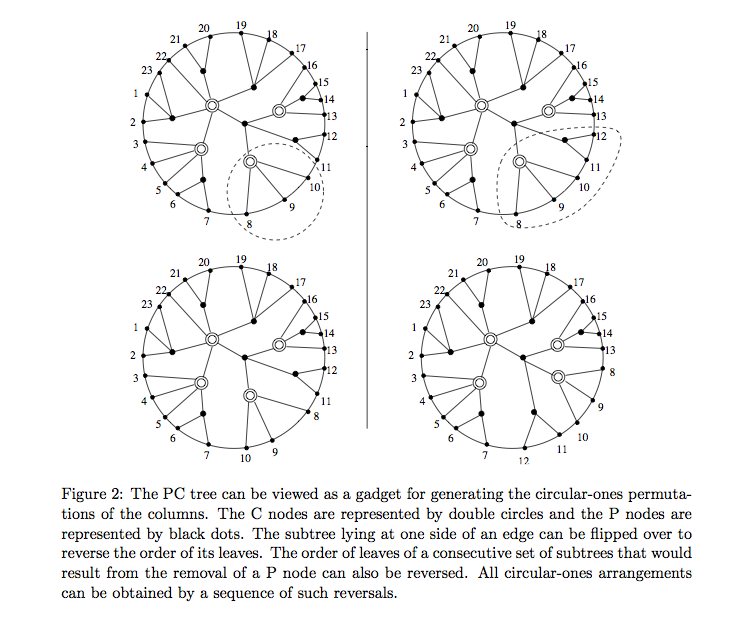
\includegraphics[scale=0.4]{../img/pctree_hm03.png}
  
  \begin{tabular}[h]{lcc}
    \pctreegraphmatrix & 
    \pctreegraphi &
    \pctreegraphii
  \end{tabular}
  \caption[\figtabsize \PCtree]{\figtabsize \PCtree with the
    associated matrix. The dark circular nodes are $P$-nodes and the
    double circular nodes are $C$-nodes.  The two \PCtrees are both
    for the same matrix. The second tree is obtained by performing the
    ``mirroring'' operation on the subtree (highlighted in the figure)
    rooted at the bottom right $C$-node.  \cite[Fig.~2.11]{d08phd}}
  \label{fig:pctree}
\end{figure}

As a data structure when \PCtree is compared with \PQtree, the
differences are, (i) it is unrooted, (ii) it represents all \CROP order of a
matrix (iii) it has $C$ nodes instead of $Q$ nodes which can be
``mirrored'' (operation defined in Definition~\ref{def:pctree}~\ref{def::pcmirror}).
The algorithms of construction of \PQtree in \cite{bl76} and that of
\PCtree in \cite{wlh01, hm03} starkly differ since the latter is a
much simplified procedure.



% WLH01 abstract:
% [..] The original implementation of the PQ-tree algorithms by Booth and
% Lueker using nine templates in each bottom-up iteration is rather
% complicated. Also the complexity analysis is rather intricate. We give
% a very simple linear time PC-tree algorithm with the following
% advantages: (1) it does not use any template; (2) at each iteration,
% it does all necessary tree-modification operations in one batch and
% does not involve the node-by-node bottom-up matching; (3) it can be
% used naturally to test the circular ones property in matrices; (4) the
% induced PQ-tree algorithm can considerably simplify Booth and Lueker’s
% modification of Lempel, Even and Cederbaum’s planarity test.

% \tnote[FYI]{ The results in cite~{bl76} on COT are based on the
%    result that interval graphs are AT-free chordal graphs cite~{lb62}?
%  No they don't seem related. this is the stupid bl lb confusion.}%



\subsection{ICPIA - a set cardinality based \COP test}
\label{sec:icpiasurvey}
In this section we see a characterization that does not use
\PQtree. \cite{nsnrs09} describes a characterization of \cop solely
based on the cardinality properties of the sets in the set system and
does not use any variants of \PQtrees.

\begin{definition}[Intersection Cardinality Preserving Interval
  Assignment (ICPIA)]
  \label{def:icpia}
  Let $\cF = \{A_i \mid A_i \subseteq U, i \in [m]\}$ be a set system
  from universe $U$ and the set of ordered pairs $\Pi = \{(A_i, B_i)
  \mid B_i  \text{ is an interval from } [n], i \in [m]\}$ be an {\em interval
    assignment} of $\cF$, then $\Pi$ is called an {\em ICPIA} if it has
  the following properties.
  \begin{enumerate}[i.]
  \item $|A_i| = |B_i|$ for all $i \in [m]$
  \item $|A_i \cap A_j| = |B_i \cap B_j|$ for all $i, j \in [m]$
  \end{enumerate}
\end{definition}

\begin{theoremsansproof}[{\cite[Th.~1]{nsnrs09}}]
  \label{th:icpia1}
  If an interval assignment $\Pi$ is feasible, then it is an ICPIA.
\end{theoremsansproof}

The necessity condition of Theorem~\ref{th:icpia1} is fairly
obvious. It turns out that it is sufficient too.  This is demostrated
by two algorithms which work as follows. The first one iterates over
the assignment $\Pi$ %set system $\cF$
and changes it in each iteration till the altered
assignment %set system
has no more overlapping intervals (intervals are the second
  element in each ordered pair of $\Pi$. Def.~\ref{def:icpia}) %sets
\cite[Alg.~1]{nsnrs09}. This is acheived by replacing two overlapping
assignment pairs $(A_i, B_i)$ and $(A_j, B_j)$ with the partitions of
$(A_i \cup A_j,B_i \cup B_j)$ induced by their overlaps -- $(A_i
\setminus A_j, B_i \setminus B_j)$, $(A_i \cap A_j, B_i \cap B_j)$ and
$(A_j \setminus A_i, B_j \setminus B_i)$.

To see it in terms of the theory explained in
Section~\ref{sec:surveycertalgo}, this results in the weak closure of
$\cF$. Let $\cF$, $\cI$ be the set system and interval
system (A set system where all the sets are intervals.),
respectively, involved in the assignment $\Pi$ and $\cF'$, $\cI'$ be
the same for the output of the algorithm $\Pi'$.  It can be observed
that $\cF' \cup \cF$ is $\overline{\cF}$ or the weak closure of
$\cF$. The analog is true for $\cI \cup \cI'$.  Moreover, this output
$\cF'$, $\cI'$ contains the strong elements of $\overline{\cF}$,
$\overline{\cI}$ respectively. It turns out that $\cI'$ is also an
interval system and that $\Pi'$ is an ICPIA \cite[Lem.~2]{nsnrs09}.

The next algorithm \cite[Alg.~2]{nsnrs09} further refines $\Pi'$ to
$\Pi''$ which represents the family of permutations that yield the
\COP orders represented by $\Pi$ of $\cF$. The subset relation Hasse
diagram of $I'$ is created with each node representing the
corresponding assignment pair of the interval from $\Pi'$. Since all intervals in
$\Pi'$ are non-overlapping, this is a tree. Notice that this means any
two intervals are now either disjoint or one is contained in the
other. Hence this tree is called a {\em containment tree}.  The
algorithm traverses this tree in post order fashion where the post
order function is to replace an assignment pair $(X,Y)$  in $\Pi'$ by their child
assignment pairs in the containment tree, say $(X_1, Y_1),(X_2, Y_2)
\ldots (X_k,Y_k)$. The result $\Pi''$ gives the
\COP order for $\Pi$. These two algorithms prove that ICPIA is a
sufficient condition for the feasibility of the interval assignment.

\begin{theoremsansproof}[{\cite[Th.~2]{nsnrs09}}]
  \label{th:icpia2}
  Let  $\cF = \{A_i \mid A_i \subseteq U, i \in [m]\}$ be a set system
  from universe $U$, $|U| = n$
  and $\Pi = \{(A_i,B_i) \mid B_i \text{ is an interval from } [n], i
  \in [m]\}$ be an ICPIA. Then there exists a permutation $\sigma: [n]
  \rightarrow [n]$ \stt $\sigma(A_i) = B_i$.
\end{theoremsansproof}

What we saw so far in this section is checking for the feasibility of
a given interval assignment. ICPIA can also be used to find an
interval assignment when only the set system $\cF$ is given. Part of
the approach is similar to the overlap component idea in \cite{fg65,
  wlh02}. Once the overlap components are factored out, they can be
independently assigned a subinterval to which the sets in the
component need to be mapped. This is simple because the overlap
components are disjoint from each other. Now the subproblem is finding
\COP order for each overlap component. In each component, the set
whose overlaps with the rest of the sets in that component forms a
single inclusion chain (see Definition~\ref{def:poset}. In this
particular reference, the set of sets is the set of overlaps.)  is
chosen first and assigned the leftmost\footnote{This is by
  convention. Rightmost can also be chosen analogously to get a
  different \COP order.} interval. The next candidate set is chosen
from this set's overlapping sets. The interval assigned is calculated
by simple intersection cardinality means. Assume that the next set
overlaps on one of the ``ends'' of the current set and calculate the
interval by shifting left or right of the current interval and
adjusting its size to match the next set's cardinality. Once the next
set is assigned an interval, the current assigned sets are all checked
for ICPIA. This is a backtracking algorithm -- if at any point ICPIA
fails, another overlapping set is chosen. If all overlapping set
attempts fail ICPIA, a different ``first set'' is chosen. This is a
remarkably simple algorithm due to its obvious simplicity in
implementation.

\section{Matrices without \COP}
\label{sec:surveycopopt}

\COP is a very beneficial property since it simplifies the structure
of the input (binary matrix or set system) leading to
efficient algorithms to otherwise hard problems.  While
Section~\ref{sec:surveycoptest} discusses matrices with \COP and how
to compute \COP orders, this section describes a couple of problems
when the input does not have \COP and identify their forbidden
substructures that prevents them from having \COP.
%describes the problems  that are
% of interest when a matrix does not have this property

\subsection{Finding forbidden submatrices}
\label{sec:forbiddensubalgo}

It is known from Theorem~\ref{th:tuckercop} that when a matrix does
not have \COP, it must have one of Tucker's forbidden submatrices (See
Section~\ref{sec:tucker} for detailed discussion on Tucker's forbidden
substructures for matrices with \COP). However, none of the \COP test
algorithms discussed in Section~\ref{sec:surveycoptest} outputs the
forbidden submatrix when the test is negative. This perhaps gives a
hint about how hard it is to find these substructures in the input
matrix. Using a reduction to the longest path problem, \cite{v85}
proves that finding a Tucker's forbidden submatrix of at least $k$
rows is NP complete. An example of an optimization problem for a
matrix without \COP is finding if deleting at most $k$ rows from input
will restore \COP. This is known to be NP complete
\cite{b75-phd}. There are several such optimization problems that try
to find ways to get \COP on the input matrix with certain alterations
and finding smallest forbidden submatrix is at the heart of these problems.


In this section we will summarize \cite{d08phd}'s approximation
algorithm for finding forbidden submatrix. We will use $\Tuckerset$ to
refer to the set of Tucker's forbidden submatrices shown in
Figure~\ref{fig:forbiddensubmatrices}.


A corollary to one of Tucker's theorems presented in
Theorem~\ref{th:tuckeratfree} is given in
Corollary~\ref{cor:tuckertheorem}. This is central to \cite{d08phd}'s
algorithm.

\begin{corollary}[{\cite[Cor.~3.1]{d08phd}}]
  \label{cor:tuckertheorem}
  A matrix $M$ has \COP \iff its representing bipartite graph $G_M$
  (the graph whose half adjacency matrix is $M$) does not contain an
  asteroidal triple whose three vertices correspond to columns of M.
\end{corollary}

Using Corollary~\ref{cor:tuckertheorem}, a forbidden submatrix can be
found as follows. For every vertex triple $x, y, z$ in $G_M$ that
correspond to columns of $M$, determine the sum of the lengths of
three shortest paths connecting each pair of these vertices (there are
3 possible pairs) avoiding the neighborhood of third vertex. If all
three paths exist, then $x, y, z$ indeed form an asteroidal
triple. Among all such triples, select the triple $u, v, w$ where the
sum is minimum and return the rows and columns of $M$ that correspond
to the vertices in the three shortest paths described earlier for this triple. This
return value forms a submatrix and it obviously must contain a
submatrix from $\Tuckerset$ because it represents an asteroidal
triple. It may be noted that this procedure does not always return a
submatrix of smallest size because the shortest paths computed may not
be vertex disjoint. The following claim shows that this certainly
gives a reasonable approximation of the solution. The claim has been
abridged to summarize the main idea behind this algorithm.
Note that a $(x,y)$-matrix is one with at most $x$ number of {\un}s in every
column and at most $y$ number of {\un}s in every row. If $x$ or $y$ is given as
$*$, it denotes that number of {\un}s is unbounded.

\begin{proposition}[{\cite[Pr.~3.1, {\em abridged}]{d08phd}}] 
  \label{prop:tuckerdomapprox}
  Let $M$ be a $(*,\Delta)$-matrix of size $m \times n$ that contains
  a forbidden submatrix $M'$ of size $m' \times n'$ from $\Tuckerset$. Then
  this algorithm computes a submatrix that belongs to $\Tuckerset$
  with at most $m'+5$ rows and $n'+3$ columns in $O(\Delta m n^2 +
  n^3)$ time.
\end{proposition}

In fact, the approximation mentioned in
Proposition~\ref{prop:tuckerdomapprox} is the worst case when
the actual solution $M'$ is of type $M_{IV}$. The approximation is
slightly better for the other types of submatrices from $\Tuckerset$,
the best case being an exact solution when $M'$ is $M_{I_k}$ or
$M_{II_k}$. Thus this algorithm works accurately when the solution is of
type $M_{I_k}$ or $M_{II_k}$.

Next, notice that Tucker matrix types $M_{IV}$ and $M_{V}$ are
constant size -- $4 \times 6$ and $4 \times 5$ respectively. Thus they
can be searched for in polynomial time even with brute force method as
Corollary~\ref{cor:mivmvpolytime} states.

\begin{corollary}[{\cite[Cor.~3.3, {\em abridged}]{d08phd}}] 
  \label{cor:mivmvpolytime}
  Let $M$ be a binary $(*, \Delta)$-matrix of size $m \times n$ and
  $M'$ be a binary matrix from $\Tuckerset$. A submatrix in $M$ that
  is isomorphic to $M'$ can be found in $O(\Delta^3m^2n^3)$ time or
  $O(\Delta^4m^2n)$ time when $M'$ is of type $M_{IV}$ or $M_V$
  respectively.
\end{corollary}

Their algorithm for finding $M_{III_k}$ type submatrix is slightly
involved and we only present here the analysis result in
Proposition~\ref{cor:miiitime}. The algorithm is derived from the
structural similarities between the first three types of Tucker
matrices and the fact that $M_{I_k}$ is a chordless cycle of length
$2k+4$.

\begin{proposition}[{\cite[Pr.~3.6]{d08phd}}] 
  \label{cor:miiitime}
  Let $M$ be a $(*,\Delta)$-matrix $M$ of size $m \times n$. Then a
  minimum size submatrix of type $M_{III_k}$ in $M$ can be found in
  $O(\Delta^3m^3n+\Delta^2m^2n^2)$ time.
\end{proposition}

All the above algorithmic results are combined to obtain the final
single algorithm for finding forbidden
submatrix. Theorem~\ref{th:forbiddenalg} gives this result.

\begin{theoremsansproof}[{\cite[Th.~3.1]{d08phd}}]
  \label{th:forbiddenalg}
  Let $M$ be a $(*,\Delta)$-matrix of size $m \times n$. A forbidden
  submatrix from $\Tuckerset$ in $M$ that has a minimum number of rows
  can be found in $O(\Delta^3m^2n\dot(m+n^2))$ time. Within the same
  time, one can also find a forbidden submatrix from $\Tuckerset$ in
  $M$ that has a minimum number of columns, a minimum number of rows
  and columns, or a minimum number of entries.
\end{theoremsansproof}

The procedure used to prove Theorem~\ref{th:forbiddenalg} is as
follows. 
\begin{enumerate}
\item Run the algorithm mentioned in
  Propostition~\ref{prop:tuckerdomapprox} to obtain a submatrix $A$
  which is an approximation of the smallest forbidden submatrix. (If
  the actual solution is $M_{I_k}$ or $M_{II_k}$ this will be an exact
  solution.)
\item Run the algorithm from Propostition~\ref{cor:miiitime} to find
  an induced $M_{III_k}$ and let this be $B$.
\item Run the algorithm from Corollary~\ref{cor:mivmvpolytime} twice
  -- once each for finding $M_{IV}$ and finding $M_{V}$. Let the
  results be $C$ and $D$ respectively.
\item Return the minimum size matrix among $A, B, C, D$ (minimum size
  being one of the following: number of rows, number of columns, sum
  of number of rows and columns, number of {\un} entries).
\end{enumerate}

In the next section we see yet another forbidden substructure for
\COP which is easier to compute.

\subsection{Incompatibility graph - a certificate for no \COP}
\label{sec:incompatibilitygr}

When a \COP test algorithm reports negative, it is hard to verify
this. While \cite{at72} gives forbidden substructures for \COP, there
are no efficient algorithms to find these strutures in a matrix. In
fact, \cite{v82} shows that even finding a forbidden submatrix with at
least $k$ rows in an input matrix is NP-complete. This was proven by
polynomially reducing the longest path problem for graphs to this
problem.

\cite{mcc04} describes another characterization for matrices without
\COP which is efficiently computable. This is done by way of an {\em
  incompatibility graph} of a set system (since \COP in
  matrices and set systems are equivalent problems as seen in
  Section~\ref{sec:surveycertalgo} we will use the term set system in
  this section, in line with \cite{mcc04}'s convention). The
construction of this graph is based on the following observation.

\begin{observation} 
  Consider elements $a, b, c \in U$ and a set system $\cF$ with
  universe $U$. If there is at least one set $S \in \cF$ \stt $a, c
  \in S$ but $b \notin S$, then it is impossible to have a \COP order
  that will place $b$ in between $a$ and $c$. \tnote[important]{also cite the
    inbetweenness problem}
\end{observation}

For the sake of argument, suppose there exists such a \COP
order. Clearly, it will not succeed in mapping $S$ to an interval
since $b \notin S$ which is a contradiction to the assumption that
this is a \COP order.  The ordered pair $(x,y)$ denotes that in the
\COP order $y$ comes after $x$. Based on above observations, this
means $(a,b)$ and $(b,c)$ are not compatible in any \COP order. So are
$(c,b)$ and $(b,a)$.  Thus a binary relation {\em is incompatible
  with} on $U \times U \setminus \{(a,a) \mid a \in U\}$ can be
defined based on the membership of elements of $U$ in the sets in
$\cF$.  \cite{mcc04} creates an incompatiblity graph with vertices
denoting ordered pairs and edges denoting the incompatibility
relation.

\begin{definition}[{\em Incompatibility graph \cite[Def.~6.1]{mcc04}}]
  \label{def:incompatibility}
  Let $\cF$ be a set system with universe $U$. Let $A_{\cF} = \{(a,b)
  \mid a, b \in U, a \ne b\}$. The {\em incompatibility graph}
  $G_I^\cF$ of $\cF$ is an undirected graph defined as follows.
%  \singlespacing
  \begin{enumerate}
  \item   The vertex set of $G_I^\cF$ is $ A_{\cF}$
  \item  The edge set of $G_I^\cF$ are pairs of the following forms
    \begin{itemize}
    \item $\{(a,b),(b,a)\}$ for all $a, b \in U$
    \item $\{(a,b),(b,c)\}$ if there exists $S \in \cF$ \stt $a, c
      \in S$ and $b \notin S$, for all $a, b, c \in U$
    \end{itemize}
  \end{enumerate}
  \dstop
\end{definition}

Thus an edge between two vertices $(a,b), (b,c)$ in $G_I^{\cF}$ means
that there exists no linear order on $U$ that can place $b$ after $a$
and place $c$ after $b$.  For any \COP order, there must not be any
incompatible pairs. Thus it must consist of an independent set $I$ of
the incompatibility graph. Moreover the independent set must have
exactly half the vertex set of $G_I^\cF$ since the \COP order must
involve all elements in $U$. Secondly, the reverse of a \COP order is
also a \COP order. Thus $A_\cF \setminus I$ must also be an
independent set. In other words, $G_I^\cF$ must be bipartite with
partitions being of equal size if $\cF$ has \COP. An odd cycle is a
forbidden structure in a bipartite graph, hence the same is forbidden
in the incompatibility graph of a set system with \COP. In other
words, if the set system has no \COP, its incompatibility graph must
have an odd cycle.  There is also a requirement on the length of this
odd cycle which is formally stated in Theorem~\ref{th:mccbipartite}.

\begin{theoremsansproof}[{\cite[Th.~6.1]{mcc04}, \cite[Corrected by
    Th.~2.6, Proof p. 44--47]{d08phd}}] 
  \label{th:mccbipartite}
  Let $\cF$ be a set family with universe $U$. Then $\cF$ has \COP
  \iff its incompatibility graph is bipartite and if it does not have
  the \COP, the incompatibility graph has an odd cycle of length at
  most $n+3$.
\end{theoremsansproof}

Searching for an odd cycle to recognize a bipartite graph is a known
and polynomially solved problem. \cite{mcc04}'s algorithm also labels
each edge of the cycle with a set from $\cF$ that documents the
incompatibility.


% \tnote[dire]{how does it give clues
%   about the $R$ node? See dom.}




%     \cite{mcc04} describes a different approach to COT. While all
%     previous COT algorithms gave the COP order if the matrix has the
%     property but exited stating negative if otherwise, this algorithm
%     gives an evidence by way of a certificate of matrix even when it
%     has no COP. This enables a user to verify the algorithm's result
%     even when the answer is negative. This is significant from an
%     implementation perspective because automated program verification
%     is hard and manual verification is more viable. Hence having a
%     certificate reinforces an implementation's credibility. Note that
%     when the matrix {\em has} COP, the COP order is the certificate.
%     The internal machinery of this algorithm is related to the
%     weighted betweenness problem addressed\tnote{in what way??} in
%     \cite{co98}.  \tnote{expand on the COP order graph creation and it
%       having to be bipartite for M to have COP. and thus an odd cycle
%       being an evidence of no COP.}







% \tnote[dire]{ -- sect 4.1 in cite:d08phd has many results surveyed. hardness
%   results, approx. results. results are usually for a class of
%   matrices $(a,b)$ where number {\un}s in columns and rows are
%   restriced to $a$ and $b$ . -- problem of flipping at most $k$
%   entries of $M$ to make it attain COP. this is NP complete
%   cite:b75-phd%
% \\(1) scite:lb62 showed that interval graphs are chordal and
%   AT-free. %
% \\couple of lines refering to tucker's submatrices. refer
%   earlier section.


% Another problem is to find the minimum number of entries in the matrix
% that can be toggled to result in a matrix with COP.  \cite{v85}
% discusses approximation of {\sc COP Augmentation} which is the problem
% of changing of the minimum number of zero entries to {\un}s so that
% the resulting matrix has COP. As mentioned earlier, this problem is
% known to be NP complete due to \cite{b75-phd}.  \tnote[pressing]{where should this go?
%   cite|tz04 (approx submatrix with COP sparse matrices)}
% }



%%%%%%%%%%%%% listing package for pretty formatting BEGIN
% \lstloadlanguages{C}
% \lstset{language=C, commentstyle=\scriptsize,
%   numberstyle=\tiny, numbers=left,               % Line numbers
%   stepnumber=2,numbersep=5pt,firstnumber=10, 
%   showstringspaces=false,                    % No explicit spaces
%   emph={printf},emphstyle=\underbar,      % Specific formatting
%   emph=[2]{sum},emphstyle=[2]\color{blue},      % Sp format (multiple)
%   emph=[3]{i},emphstyle=[3]\color{red}      % Sp format (multiple)
%   } 

%   \begin{singlespacing}
%     % Text inside "lstlisting" env is verbatim.
%     \begin{lstlisting}[keywordstyle=\textbf]      
% int sum;
% int i; /* for loop variable */ 
% sum = 0; 
% for (i=0, i<n; i++) { 
%   sum += a[i]; 
% } 
% printf{"This is stupid."}
%     \end{lstlisting}
%   \end{singlespacing}

%%%%%%%%%%%%% listing package for pretty formatting END


\chapter[Tree Path Labeling]{Tree Path Labeling of Path
  Hypergraphs -- New Results}
\label{ch:myresearch}

This chapter documents all the new results obtained by us
in the area of tree path labeling of path hypergraphs which is the
parent problem addressed in this thesis.

Section~\ref{sec:myresearchintro} recalls the idea of tree path
labeling. The necessary preliminaries with definitions etc. are
presented in Section~\ref{ch:prelims}. Section~\ref{sec:feasible}
documents the characterization of a feasible path labeling for any
path labeling from any target trees. Section~\ref{sec:spltargettree}
describes two special cases where the target tree is of a particular
family of trees. The first one is shown to be equivalent to COP
testing in Section~\ref{sec:icpplicpia}. Section~\ref{sec:ksubdivstar}
discusses the second special case and presents a polynomial time
algorithm to find the tree path labeling of a given set system from a
given \kstar. Section~\ref{sec:norestraint} discusses the plain
vanilla version where the target tree has no restrictions and the
algorithm to find a feasible TPL, if any, in this case.


\section[Summary of problems]{Summary of Proposed Problems}
\label{sec:myresearchintro}
In Section~\ref{sec:motive} we see that consecutive-ones property and
its equivalent problem of interval labeling of a hypergraph is a
special case of the general problem of tree path labeling of path
hypergraphs.  The problem of consecutive-ones property testing can be
easily seen as a simple constraint satisfaction problem involving a
hypergraph or a system of sets from a universe. Every column (row) of
the binary matrix can be converted into a set of non-negative integers
which are the indices of the rows (columns) with {\un}s in that column
(row). When observed in this context, if the matrix has the COP on
columns (rows), a reordering of its rows (columns) will result in sets
that have only consecutive integers. In other words, the sets after
applying the COP row (column) permutation are intervals.  In this
form, one can see that this is indeed the problem of finding interval
assignments to the given set system \cite{nsnrs09} with a single
permutation of the universe (set of row or column indices for COP of
columns or rows, respectively) which permutes each set to an
interval. The result in \cite{nsnrs09} characterizes interval
assignments to the sets which can be obtained from a single
permutation of the universe. The cardinality of the interval
assigned to it must be same as the cardinality of the set, and the
intersection cardinality of any two sets must be same as the
intersection cardinality of the corresponding intervals. This is a
necessary and sufficient condition. \tnote{(ICPIA) put reference to
  survey chapter}

Naturally, intervals are paths from a tree with maximum degree
two. Thus the interval assignment problem can be generalized into path
assignment problem from any tree. We refer to this as the {\em tree
  path labeling problem of path hypergraphs}. This is analogous to the
interval labeling problem in literature \cite{kklv10} to interval
hypergraphs. To elaborate, the problem is defined as follows -- given
a hypergraph $\cF$ from universe (hypergraph vertex set) $U$ and a target tree
$T$, does there exist a bijection $\phi$ from $U$ to the vertices of $T$ such
that for each hyperedge when applied to its elements, $\phi$ gives a path on
$T$.  More formally, the problem definition is as defined by \CFTPL.

{\small
  \begin{minipage}[h]{5in}
    \vspace{2mm}
    {\large \CFTPL}\\
    \begin{tabular}[t]{l|l}
      \hline\\
      {\tt Input} & 
      \begin{minipage}[t]{\probdefwidth}
        A hypergraph $\cF$ with vertex set $U$ and a tree $T$.\\
      \end{minipage}\\

      {\tt Question} &
      \begin{minipage}[t]{\probdefwidth}
        Does there exist a set of paths $\cP$ from $T$ and a bijection
        $\cl$~$:$~$\cF \rightarrow \cP$, such that {\FTPL} returns
        {\bf true} on $(\cF, T, \cl)$.
      \end{minipage}\\
    \end{tabular}
  \end{minipage}\\
}


To characterize a feasible TPL, we consider the case where a tree path
labeling is also given as input and we are required to test if the
given labeling is feasible. This is defined by the \FTPL problem.

%\begin{tabular}[t]{c}
{\small
\begin{minipage}[h]{5in}
 % \begin{singlespace}
 \vspace{2mm}
 {\large \FTPL}\\
 \begin{tabular}[t]{l|l}
 \hline\\
    {\tt Input} & 
    \begin{minipage}[t]{\probdefwidth}
      A hypergraph $\cF$ with vertex set $U$, a tree $T$, a set of
      paths $\cP$ from $T$ and a
      bijection $\cl$~$:$~$\cF \rightarrow \cP$.\\
    \end{minipage}\\
    {\tt Question} &
    \begin{minipage}[t]{\probdefwidth}
      Does there exist a bijection $\phi$~$:$~$U \rightarrow V(T)$
      such that $\phi$ when applied on any hyperedge in $\cF$ will
      give
      the path mapped to it by the given tree path labeling $\cl$.\\
      { i.e., $\cl(S) = \{\phi(x) \mid x \in S\}$, for every hyperedge
        $S \in \cF$.}
    \end{minipage}\\
  \end{tabular}
  % \end{singlespace}
\end{minipage}\\
}
% \end{tabular}

Section~\ref{sec:feasible} discusses \FTPL and presents an algorithmic
characterization for a feasible TPL.

With respect to computing a feasible TPL, as suggested by \CFTPL
problem, we were unable to discover an efficient algorithm for
it. Hence we consider two special cases of the same -- namely, \CFTPLINT
and \CFTPLKTREE on special target trees, namely, intervals and \kstars,
respectively.  Section~\ref{sec:spltargettree} discusses these
problems.

{\small
  \begin{minipage}[h]{5in}
    % \begin{singlespace}
    \vspace{2mm}
    {\large \CFTPLINT}\\
    \begin{tabular}[t]{l|l}
      \hline\\
      {\tt Input} & 
      \begin{minipage}[t]{\probdefwidth}
        A hypergraph $\cF$ with vertex set $U$ and a tree $T$ with
        maximum degree 2.\\
      \end{minipage}\\
      {\tt Question} &
      \begin{minipage}[t]{\probdefwidth}
        Does there exist a set of paths $\cP$ from $T$ and a bijection
        $\cl$~$:$~$\cF \rightarrow \cP$, such that {\FTPL} returns
        {\bf true} on $(\cF, T, \cl)$.
      \end{minipage}\\
    \end{tabular}
    % \end{singlespace}
  \end{minipage}\\
}

{\small
  \begin{minipage}[h]{5in}
    % \begin{singlespace}
    \vspace{2mm}
    {\large \CFTPLKTREE}\\
    \begin{tabular}[t]{l|l}
      \hline\\
      {\tt Input} & 
      \begin{minipage}[t]{\probdefwidth}
        A hypergraph $\cF$ with vertex set $U$ such that every
        hyperedge
        $S \in \cF$ is of cardinality at most $k+2$ and a {\kstar} $T$.\\
      \end{minipage}\\
      {\tt Question} &
      \begin{minipage}[t]{\probdefwidth}
        Does there exist a set of paths $\cP$ from $T$ and a bijection
        $\cl$~$:$~$\cF \rightarrow \cP$, such that {\FTPL} returns
        {\bf true} on $(\cF, T, \cl)$.
      \end{minipage}\\
    \end{tabular}
    % \end{singlespace}
  \end{minipage}\\
}

\CFTPLINT is nothing but the consecutive-ones property testing
problem.

An algorithm for \CFTPL on general trees which is less efficient than
polynomial time is presented in
Section~\ref{sec:norestraint}. \tnote[minor]{put some more description
  here. refer WG11.}

\remove[minor]{We focus on the question of generalizing the notion of an
  ICPIA cite-nsnrs09 to characterize feasible path assignments.  We
  show that for a given set system $\cF$, a tree $T$, and an
  assignment of paths from $T$ to the sets, there is a feasible
  bijection between $U$ and $V(T)$ if and only if all intersection
  cardinalities among any three sets (not necessarily distinct) is
  same as the intersection cardinality of the paths assigned to them
  and the input runs a filtering algorithm (described in this paper)
  successfully.  This characterization is proved constructively and it
  gives a natural data structure that stores all the relevant feasible
  bijections between $U$ and $V(T)$.  Further, the filtering algorithm
  is also an efficient algorithm to test if a tree path labeling to
  the set system is feasible.  This generalizes the result in
  cite-nsnrs09.}


\section[Preliminaries]{Preliminaries to new results}
\label{ch:prelims}

This section states definitions and basic facts necessary in the scope
of this document.

\subsection{Hypergraph Preliminaries}

\begin{definition}[Set systems and hypergraphs] 
  \noindent 
  The set $\F \subseteq (2^{U} \setminus \emptyset)$ is a {\em set
    system} of a universe $U$ with $|U| = n$.  The {\em support} of a
  set system $\F$ denoted by $\supt{\cF}$\tnote[minor]{change all supp
    references to supt command} is the union of all the sets in $\F$;
  $supp(\F) = \bigcup_{S \in \F}S$. For the purposes of this paper, a
  set system is required to ``cover'' the universe; $ supp(\cF) = U$.
 
  \noindent
  A set system $\cF$ can also be visualized as a {\em hypergraph}
  whose vertex set is $supp(\cF)$ and hyperedges are the sets in
  $\cF$. This is a known representation for
  interval systems in literature \cite{bls99,kklv10}.  We extend this
  definition here to path systems. Due to the equivalence of set
  system and hypergraph in the scope of this paper, we drop the
  subscript $_H$ in the notation and refer to both the structures by
  $\cF$.

  \noindent
  The {\em intersection graph}\, $\bI(\cF)$ of a hypergraph
  $\cF$ is a graph such that its vertex set has a bijection to $\cF$
  and there exists an edge between two vertices \iff their
  corresponding hyperedges have a non-empty intersection \cite{mcg04}.

  \noindent 
  Two hypergraphs $\cF'$, $\cF''$ are said to be {\em isomorphic} to
  each other, denoted by $\cF' \cong \cF''$, \iff there exists a
  bijection $\phi: supp(\cF') \rightarrow supp(\cF'')$ such that for
  all sets $A \subseteq supp(\cF')$, $A$ is a hyperedge in $\cF'$ \iff
  $B$ is a hyperedge in $\cF''$ where $B = \{\phi(x) \mid x \in A\}$
  \cite{kklv10}, written as $B=\phi(A)$.  This is called {\em
    hypergraph isomorphism}.  
\end{definition}

\begin{definition}[Path Hypergraph from a Tree]
  The graph $T$ represents a {\em target tree} with same number of
  vertices as elements in $U$; $|V(T)|=|U|=n$.  A {\em path system}\,
  $\cP$ is a set system of paths from $T$; $\cP \subseteq \{P \mid P
  \subseteq V, \text{ } T[P] \text{ is a path} \}$.  This generalizes
  the fact, from the literature \cite{bls99,kklv10}, that intervals
  can be viewed as sub-paths of a path.

  \noindent
  If the intersection graphs of $\cF$ and $\cP$ (a path system) are
  isomorphic, $\bI(\cF) \cong \bI(\cP)$, then the associated bijection
  $\cl: \cF \rightarrow \cP$ due to this isomorphism is called a {\em
    path labeling} of the hypergraph $\cF$.\footnote{Note that there
    are two kinds of isomorphisms here.  One is the isomorphism of
    intersection graphs on $\cF$ and $\cP$, i.e. $\bI(\cF)$ and
    $\bI(\cP)$ respectively. Second is the isomorphism between the
    hypergraphs $\cF$ and $\cP$.} 

% The subset of the path labeling that
%   maps elements of the universe to paths that contain only a leaf the
%   target tree is  known as a {\em leaf labeling}.
%   \ie if the target tree has the set of $k$ leaves $L = \{v_i, i \in
%   [k]\}$, then 
% $\cl': \rightarrow U' \rightarrow L$ is a leaf labeling where $U'
% \subseteq U$, $|U'| = k$.

  

%   $\cL_0 = \{ (x_i,v_i) \mid x_i \in
%   U, v_i \in T, x_i \ne x_j, v_i \ne v_j, i \ne j, i,j \in [k] \}$
%   where $k$ is the number of leaves in $T$
  

  \noindent
  \add{To illustrate further, let $\cg: V(\cF) \rightarrow V(\cP)$ be
    the above mentioned isomorphism where $V(\cF)$ and $V(\cP)$ are
    the vertex sets that represent the hyperedges for each hypergraph
    respectively, $V(\cF) = \{ v_S \mid S \in \cF\}$ and $V(\cP) = \{
    v_P \mid P \in \cP\}$. Then the path labeling $\cl$ is defined as
    follows: $\cl(S_1) = P_1$ iff $\cg (v_{S_1}) = v_{P_1}$.  Just to
    emphasize, for a path labeling $\cl$ of $\cF$ with $\cP$ as the
    path system, $\cF^\cl$ is same as $\cP$.  The path system $\cP$
    may be alternatively denoted in terms of $\cF$ and $\cl$ as
    $\cF^\cl$. In most scenarios in this paper, what is given are the
    pair $(\cF, \cl)$ and the target tree $T$; hence this notation
    will be used more often.}

  \noindent
  If $\cF \cong \cP$ where $\cP$ is a path system, then $\cF$ is
  called a {\em path hypergraph} and $\cP$ is called {\em path
    representation} of $\cF$. If this isomorphism is $\phi: supp(\cF)
  \rightarrow V(T)$, then it is clear that there is an {\em induced
    path labeling} $\cl_\phi: \cF \rightarrow \cP$ to the set system;
  $\cl_\phi(S) = \set{y \mid y = \phi(x), x \in S}$ for all $S \in
  \cF$. Recall that $supp(\cP) = V(T)$.

  \noindent
  \add{A graph} $G$ is a {\em path graph} if it is isomorphic to the
  intersection graph $\bI(\cP)$ of a path system $\cP$.  This
  isomorphism gives a bijection $\cl': V(G) \rightarrow
  \cP$. Moreover, for the purposes of this paper, we require that in a
  path labeling, $supp(\cP) = V(T)$.  If graph $G$ is also isomorphic
  to $\bI(\cF)$ for some hypergraph $\cF$, then clearly there is a
  bijection $\cl: \cF \rightarrow \cP$ such that $\cl(S) = \cl'(v_S)$
  where $v_S$ is the vertex corresponding to set $S$ in $\bI(\cF)$ for
  any $S \in \cF$. This bijection $\cl$ is called the {\em path
    labeling} of the hypergraph $\cF$ and the path system $\cP$ may be
  alternatively denoted as $\cF^\cl$.

  \noindent
  A path labeling $(\cF, \cl)$ is defined to be {\em feasible} if $\cF
  \cong \cF^\cl$ and this hypergraph isomorphism $\phi: supp(\cF)
  \rightarrow supp(\cF^\cl)$ induces a path labeling $\cl_\phi: \cF
  \rightarrow \cF^\cl$ such that $\cl_\phi = \cl$.  \add{In this
    work}, we are given as input $\cF$ and a tree $T$, and the
  question is whether there is a path labeling $\cl$ to a set of paths
  in $T$.  We refer to such a solution path system by $\cF^\cl$.  A
  path labeling $(\cF, \cl)$ is defined to be {\em feasible} if
  % $\cF \cong \cF^\cl$ and this
  there is a hypergraph isomorphism $\phi: supp(\cF) \rightarrow
  supp(\cF^\cl)=V(T)$ induces a path labeling $\cl_\phi: \cF
  \rightarrow \cF^\cl$ such that $\cl_\phi = \cl$.
\end{definition}


\begin{definition}[Overlap Graphs and Marginal Hyperedges]
  An {\em overlap graph}\, $\bO(\cF)$ of a hypergraph $\cF$ is a graph
  such that its vertex set has a bijection to $\cF$ and there exists
  an edge between two of its vertices \iff their corresponding
  hyperedges overlap. Two hyperedges $S$ and $S'$ are said to {\em
    overlap}, denoted by $S \overlap S'$, if they have a non-empty
  intersection and neither is contained in the other; $S \overlap S'
  \text{ \iff } S \cap S' \ne \emptyset, S \nsubseteq S', S'
  \nsubseteq S$. Thus $\bO(\cF)$ is a spanning subgraph of $\bI(\cF)$
  and not necessarily connected. Each connected component of
  $\bO(\cF)$ is called an {\em overlap component}.

  \noindent
  A hyperedge $S \in \cF$ is called {\em marginal} if for all $S'
  \overlap S$, the overlaps $S \cap S'$ form a single inclusion chain
  \cite{kklv10}. Additionally, if $S$ is such that it is contained in
  no other marginal hyperedge in $\cF$, then it is called {\em
    super-marginal}.
\end{definition}

\begin{definition}[$k$-subdivided star] 
  A {\em star} graph is a
  complete bipartite graph $K_{1,p}$ which is clearly a tree and $p$
  is the number of leaves. The vertex with maximum degree is called
  the {\em center} of the star and the edges are called {\em rays} of
  the star. A {\em $k$-subdivided star} is a star with all its rays
  subdivided exactly $k$ times. The definition of a {\em ray of a
    $k$-subdivided star} is extended to the path from the center to a
  leaf. It is clear that all rays are of length $k+2$.
\end{definition}


\temptext{ --- WG11 begin --- }

\remove[dire]{
A path assignment }% $\A$ to $\F$ is defined as a set assignment
% where second universe is the vertex set $V$ of a given tree $T$ and
% every second subset in the ordered pairs is a path in this
% tree. Formally, the definition is as follows. 
% \begin{align*}
%   \A = \{ (S_i,P_i) \mid S_i \in \F, P_i \subseteq V \text{
%     s.t. }T[P_i] \text{ is a path, } i \in I \}
% \end{align*}
% In other words, $P_i$ is the path on the tree $T$ assigned to $S_i$ in
% $\A$. As mentioned before for set systems, the paths cover the whole
% tree, i.e. $\bigcup_{i \in I}P_i = V$ \\

% Generalizing the definition of { feasibility} in cite{nsnrs09} to
% a set assignment, a path assignment $\A$ is defined to be {
%   feasible} if there exists a bijection defined as follows.
% \begin{align}
%   \sigma: U \rightarrow V(T), \text{ such that }\sigma(S_i) = P_i
%   \text{ for all } i \in I, \sigma \text{ is a bijection}
%   \label{eq:stf}
% \end{align}


\begin{definition}[Partially ordered sets]
  
Let $X$ be a partially ordered set with $\preccurlyeq$ being the
partial order on $X$.  $mub(X)$ represents an element in $X$ which is
a maximal upper bound on $X$.  $X_m \in X$ is a maximal upper bound of
$X$ if $\nexists X_q \in X$ such that $X_m
\preccurlyeq X_q$. 
\end{definition}


\noindent
The set $I$ represents the index set $[m]$. If index $i$ is used
without further qualification, it is meant to be $i \in I$. Any
function, if not defined on a domain of sets, when applied on a set is
understood as the function applied to each of its elements. i.e. for
any function $f$ defined with domain $U$, the abuse of notation is as
follows; $f(S)$ is used instead of $\hat f(S)$ where
$\hat f(S) = \{y \mid y = f(x), x \in S\}$. \\

\noindent
When refering to a tree as $T$ it could be a reference to the tree
itself, or the vertices of the tree. This will be clear from the
context.\\

\noindent
Finally, an in-tree is a directed rooted tree in which all edges are
directed toward to the root.

\temptext{ --- WG11 end --- }

\section[Characterization of FTPL]{Characterization of Feasible Tree Path Labeling}
\label{sec:feasible}

\tnote{\sc refer to Problem Defs here}
In this section we give an algorithmic characterization of the
feasibility of a tree path labeling.  Consider a path labeling $(\cF,
\cl)$ on the given tree $T$. We call $(\cF, \cl)$ an {\em Intersection
  Cardinality Preserving Path Labeling (ICPPL)} if it has the
following properties.

\begin{enumerate}[{(\icpplpr\ }i)]
\item \label{pr:i} $|S| = |\cl(S)|$ for all $S \in \cF$
  % \vspace{\topshrink}
\item \label{pr:ii}$|S_1 \cap S_2| = |\cl(S_1) \cap \cl(S_2)|$ for all
  distinct $S_1, S_2 \in \cF$
  % \vspace{\topshrink}
\item \label{pr:iii}$|S_1 \cap S_2 \cap S_3| = |\cl(S_1) \cap \cl(S_2)
  \cap \cl(S_3)|$ for all distinct $S_1, S_2, S_3 \in \cF$
\end{enumerate}


The following lemma is useful in subsequent arguments.
\begin{lemma}
  \label{lem:setminuscard}
  If $\cl$ is an ICPPL, and $S_1, S_2, S_3 \in \cF$, then $|S_1 \cap
  (S_2 \setminus S_3)| = |\cl(S_1) \cap (\cl(S_2) \setminus
  \cl(S_3))|$.
\end{lemma}
\begin{proof}\thesisspacing%[Proof of Lemma~\ref{lem:setminuscard}]
  Let $P_i = \cl(S_i)$, for all $1 \le i \le 3$.  $|S_1 \cap (S_2
  \setminus S_3)| = |(S_1 \cap S_2) \setminus S_3| = |S_1 \cap S_2| -
  |S_1 \cap S_2 \cap S_3|$. Due to properties (ii) and (iii) of ICPPL,
  $|S_1 \cap S_2| - |S_1 \cap S_2 \cap S_3| = |P_1 \cap P_2| - |P_1
  \cap P_2 \cap P_3| = |(P_1 \cap P_2) \setminus P_3| = |P_1 \cap (P_2
  \setminus P_3)|$. %\qed
\end{proof}


In the remaining part of this section we show that $(\cF, \cl)$ is
feasible if and only if it is an ICPPL and
Algorithm~\ref{al:icppl-find-isomorph} returns a non-empty path
hypergraph isomorphism
function. Algorithm~\ref{al:icppl-find-isomorph} recursively does two
levels of filtering of $(\cF, \cl)$ to make it simpler in terms of set
intersections while retaining the set of isomorphisms, if any, between
$\cF$ and $\cF^\cl$.
% One direction of this claim isclear: that if a path labeling is
% feasible, then all intersection cardinalities are preserved,
% i.e. the path labeling is an ICPPL. Algorithm~\ref{al:filterone}
% \annote{has no premature exit condition hence any input will go
%   through it}{Prove that the filtered sets has ICPPL \iff input PL
%   has ICPPL?}. Algorithm~\ref{al:filtertwo} has an exit condition at
% line~\ref{xempty}. It can be easily verified that $X$ cannot be
% empty if $\cl$ is a feasible path labeling. The reason is that a
% feasible path labeling has an associated bijection between
% $supp(\cF)$ and $V(T)$ \remove{i.e. $supp(\cF^{\cl})$} such that the
% sets map to paths, ``preserving'' the path labeling.  The rest of
% the section is devoted to constructively proving that it is
% sufficient for a path labeling to be an ICPPL and pass the two
% filtering algorithms.  To describe in brief, the constructive
% approaches refine an ICPPL iteratively, such that at the end of each
% iteration we have a ``filtered'' path labeling, and finally we have
% a path labeling that defines a family of bijections from $supp(\cF)$
% to $V(T)$\remove{ i.e. $supp(\cF^{\cl})$}.
First, we present Algorithm~\ref{al:filterone} which describes {\tt
  filter\_1}, and prove its correctness.  This algorithm refines the
path labeling by processing pairs of paths in $\cF^\cl$ that share a
leaf until no two paths in the new path labeling share any leaf.

\begin{algorithm}[h]
  \caption{Refine ICPPL {\tt filter\_1($\cF, \cl, T$)}}
  \label{al:filterone} % {perms}
  \begin{algorithmic}[\lndisplay]
    \STATE $\cF_0 \assign \cF$, $\cl_0(S) \assign \cl(S)$ for all $S \in \cF_0$\\
    \STATE $j \assign 1$\\
    \WHILE {there is $S_1, S_2 \in \cF_{j-1}$ such that
      $\cl_{j-1}(S_1)$ and $\cl_{j-1}(S_2)$ have a common leaf in
      $T$}\label{shareleaf} \STATE $\cF_j \assign (\cF_{j-1} \setminus
    \{S_1, S_2\}) \cup \{S_1 \cap S_2, S_1 \setminus S_2, S_2
    \setminus S_1 \}$ \label{setbreak} \COMMENT {Remove $S_1$, $S_2$
      and add the ``filtered'' sets} \STATE {\bf for} every $S \in
    \cF_{j-1}$ s.t. $S \ne S_1$ and $S \ne
    S_2$ {\bf do} $\cl_j(S) \assign \cl_{j-1}(S)$ {\bf end for}\\

    \STATE $\cl_j(S_1 \cap S_2) \assign \cl_{j-1}(S_1) \cap
    \cl_{j-1}(S_2)$ \COMMENT {Carry forward the path labeling for all
      existing sets other than $S_1$, $S_2$} \STATE $\cl_j(S_1
    \setminus S_2) \assign \cl_{j-1}(S_1) \setminus \cl_{j-1}(S_2)$
    \COMMENT {Define path labeling for new sets} \STATE $\cl_j(S_2
    \setminus S_1) \assign \cl_{j-1}(S_2) \setminus \cl_{j-1}(S_1)$

    \IF{$(\cF_j, \cl_j)$ does not satisfy (\icpplpr~\ref{pr:iii}) of
      ICPPL}
    \label{ln:3waycheck}
    \STATE {\bf exit} \label{ln:exit1} \\
    \ENDIF

    \STATE $j \assign j+1$\\
    \ENDWHILE
    \STATE $\cF' \assign \cF_j$, $\cl' \assign \cl_j$\\
    \RETURN $(\cF', \cl')$
  \end{algorithmic}
\end{algorithm}

\begin{lemma}
  \label{lem:feasible}
  In Algorithm~\ref{al:filterone}, if input $(\cF, \cl)$ is a feasible path
  assignment then at the end of $j$th iteration of the {\bf while}
  loop, $j \ge 0$, $(\cF_j, \cl_j)$ is a feasible path assignment.
\end{lemma}
\begin{proof}\thesisspacing%[Proof of Lemma~\ref{lem:feasible}]
  We will prove this by mathematical induction on the number of
  iterations. The base case $(\cF_0, \cl_0)$ is feasible since it is
  the input itself which is given to be feasible. Assume the lemma is
  true till $j-1$th iteration. \ie every hypergraph isomorphism $\phi:
  supp\left(\cF_{j-1}\right) \rightarrow V\left(T \right)$ that
  defines $(\cF, \cl)$'s feasibility, is such that the induced path
  labeling on $\cF_{j-1}$, say denoted by $\cl_{\phi[{\cF_{j-1}}]}$, is equal to
  $\cl_{j-1}$. We will prove that $\phi$ is also the bijection that
  makes $(\cF_j, \cl_j)$ feasible. Note that $supp(\cF_{j-1}) =
  supp(\cF_{j})$ since the new sets in $\cF_j$ are created from basic
  set operations to the sets in $\cF_{j-1}$ adding or removing no
  elements. For the same reason and $\phi$ being a bijection, it is
  clear that when applying the $\phi$-induced path labeling on
  $\cF_j$, $ \cl_{\phi[{\cF_{j}}]}(S_1 \setminus S_2) =
  \cl_{\phi[{\cF_{j-1}}]}(S_1) \setminus
  \cl_{\phi[{\cF_{j-1}}]}(S_2)$. Now observe that $ \cl_j(S_1
  \setminus S_2) = \cl_{j-1}(S_1) \setminus \cl_{j-1}(S_2) =
  \cl_{\phi[{\cF_{j-1}}]}(S_1) \setminus
  \cl_{\phi[{\cF_{j-1}}]}(S_2)$. Thus the induced path labeling
  $\cl_{\phi[{\cF_{j}}]} = \cl_{j}$.  %\qed
\end{proof}



\begin{lemma}
  \label{lem:invar1} In Algorithm~\ref{al:filterone}, at the end of $j$th
  iteration, $j \ge 0$, of the {\bf while} loop, the following
  invariants are maintained.
  \begin{enumerate}[I {\ }] %\vspace{\topshrink}
  \item $\cl_j(R)$ is a path in $T$, \ \ \ \ \ \ \ \ \ \ \ \ \ \ \ \ \
    \ \ \ \ \ \ \ \ \ \ for all $R \in \cF_j$%\vspace{\topshrink}
  \item $|R| = |\cl_j(R)|$, \ \ \ \ \ \ \ \ \ \ \ \ \ \ \ \ \ \ \ \ \
    \ \ \ \ \ \ \ \ \ \ \ \ \ \ \ for all $R \in
    \cF_j$%\vspace{\topshrink}
  \item $|R \cap R'| = |\cl_j(R) \cap \cl_j(R')|$, \ \ \ \ \ \ \ \ \ \
    \ \ \ \ \ \ \ \ \ \ for all $R, R' \in \cF_j$%\vspace{\topshrink}
  \item $|R \cap R' \cap R''|=|\cl_j(R) \cap \cl_j(R') \cap
    \cl_j(R'')|$, \ \ \ for all $R, R', R'' \in \cF_j$
  \end{enumerate}
\end{lemma}

\begin{proof}\thesisspacing
  Proof is by induction on the number of iterations, $j$. In this
  proof, the term ``new sets'' will refer to the sets added to $\cF_j$
  in $j$th iteration in line~\ref{setbreak} of Algorithm~\ref{al:filterone},
  $S_1 \cap S_2, S_1 \setminus S_2, S_2 \setminus S_1$ and its images
  in $\cl_j$ where $\cl_{j-1}(S_1)$
  and $\cl_{j-1}(S_2)$ intersect and share a leaf.\\
  The invariants are true in the base case $(\cF_0, \cl_0)$, since it
  is the input ICPPL.  Assume the lemma is true till the $j-1$th
  iteration. Let us consider the possible cases for each of the above
  invariants for the $j$th iteration.
  
  \begin{enumerate}[\xbullet]
  \item {\em Invariant} I/II
    \begin{enumerate}[{I/II}a $|$] % \textbullet
    \item {\em $R$ is not a new set.} It is in $\cF_{j-1}$. Thus
      trivially true by induction hypothesis.
    \item {\em $R$ is a new set.} If $R$ is in $\cF_{j}$ and not in
      $\cF_{j-1}$, then it must be one of the new sets added in
      $\cF_j$. In this case, it is clear that for each new set, the
      image under $\cl_j$ is a path since by definition the chosen
      sets $S_1$, $S_2$ are from $\cF_{j-1}$ and due to the while loop
      condition, $\cl_{j-1}(S_1)$, $\cl_{j-1}(S_2)$ have a
      common leaf. Thus invariant I is proven.\\
      Moreover, due to induction hypothesis of invariant III and the
      definition of $l_j$ in terms of $l_{j-1}$, invariant II is
      indeed true in the $j$th iteration for any of the new sets.  If
      $R = S_1 \cap S_2$, $|R| = |S_1 \cap S_2| = |\cl_{j-1}(S_1) \cap
      \cl_{j-1}(S_2)| = |\cl_j(S_1 \cap S_2)| = |\cl_j(R)|$.  If $R =
      S_1 \setminus S_2$, $|R| = |S_1 \setminus S_2| = |S_1| - |S_1
      \cap S_2| = |\cl_{j-1}(S_1)| - |\cl_{j-1}(S_1) \cap
      \cl_{j-1}(S_2)| = |\cl_{j-1}(S_1) \setminus \cl_{j-1}(S_2)| =
      |\cl_j(S_1 \setminus S_2)|
      = |\cl_j(R)|$. Similarly if $R = S_2 \setminus S_1$.\\
    \end{enumerate}
  \item {\em Invariant} III
    \begin{enumerate}[{III}a $|$]
    \item {\em $R$ and $R'$ are not new sets.} It is in
      $\cF_{j-1}$. Thus trivially true by induction hypothesis.
    \item {\em Only one, say $R$, is a new set.} Due to invariant IV
      induction hypothesis, Lemma~\ref{lem:setminuscard} and
      definition of $\cl_j$, it follows that invariant III is true no
      matter which of the new sets $R$ is equal to. If $R = S_1 \cap
      S_2$, $|R \cap R'| = |S_1 \cap S_2 \cap R'| = |\cl_{j-1}(S_1)
      \cap \cl_{j-1}(S_2) \cap \cl_{j-1}(R')| = |\cl_j(S_1 \cap S_2)
      \cap \cl_j(R')| = |\cl_j(R) \cap \cl_j(R')|$.  If $R = S_1
      \setminus S_2$, $|R \cap R'| = |(S_1 \setminus S_2) \cap R'| =
      |(\cl_{j-1}(S_1) \setminus \cl_{j-1}(S_2)) \cap \cl_{j-1}(R')| =
      |\cl_{j}(S_1 \cap S_2) \cap \cl_{j}(R')| = |\cl_{j}(R) \cap
      \cl_{j}(R')|$. Similarly, if $R = S_2 \setminus
      S_1$. Note $R'$ is not a new set.\\

    \item {\em $R$ and $R'$ are new sets.} By definition, the new sets
      and their path images in path label $\cl_j$ are disjoint so $|R
      \cap R'| = |\cl_j(R) \cap \cl_j(R)| = 0$. Thus case proven.
    \end{enumerate}
  \item {\em Invariant} IV
    
    Due to the condition in line~\ref{ln:3waycheck}, this invariant is
    ensured at the end of every iteration.
    % \begin{enumerate} [{Case 3.}1:]
    % \item {\em $R$, $R'$ and $R''$ are not new sets.} Trivially true
    %   by induction hypothesis.
    % \item {\em Only one, say $R$, is a new set.}  If $R = S_1 \cap
    %   S_2$, from Lemma~\ref{lem:fourpaths} and invariant III
    %   hypothesis, this case is proven. Similarly if $R$ is any of
    %   the other new sets, the case is proven by also using Lemma
    %   ~\ref{lem:setminuscard}.
    % \item {\em At least two of $R, R', R''$ are new sets.}  The new
    %   sets are disjoint hence this case is vacuously true.
    % \end{enumerate}
  \end{enumerate} %\qed
  % \vspace{-6mm}
\end{proof}

\begin{lemma}
  \label{lem:noexit1}
  If the input ICPPL $(\cF, \cl)$ to Algorithm~\ref{al:filterone} is
  feasible, then the set of hypergraph isomorphism functions that
  defines $(\cF, \cl)$'s feasibility is the same as the set that
  defines $(\cF_j, \cl_j)$'s feasibility, if any.  Secondly, for any
  iteration $j > 0$ of the {\em \bf while} loop, the {\em \bf exit}
  statement in line~\ref{ln:exit1} will not execute.
\end{lemma}
\begin{proof}\thesisspacing
  Since $(\cF,\cl)$ is feasible, by Lemma~\ref{lem:feasible}
  $(\cF_j,\cl_j)$ for every iteration $j > 0$ is
  feasible.  % Therefore,
  % every hypergraph isomorphism $\phi: supp(\cF) \rightarrow V(T)$
  % that induces $\cl$ on $\cF$ also induces $\cl_{j-1}$ and $\cl_{j}$
  % on $\cF_{j-1}$ and $\cF_{j}$ respectively, i.e.,
  % $\cl_{\phi[\cF_{j-1}]} = \cl_{j-1}$ and $\cl_{\phi[\cF_j]} =
  % \cl_j$. Thus it can be seen that for all $x \in supp(\cF)$, for
  % all $v \in V(T)$ the following hold true.
  Also, every hypergraph isomorphism $\phi: supp(\cF) \rightarrow
  V(T)$ that induces $\cl$ on $\cF$ also induces $\cl_{j}$ on
  $\cF_{j}$, i.e., $\cl_{\phi[\cF_j]} = \cl_j$. Thus it can be seen
  that for all $x \in supp(\cF)$, for all $v \in V(T)$, if $(x,v) \in
  \phi$ then $v \in \cl_{j}(S)$ for all $S \in \cF_{j}$ such that $x
  \in S$.
  % the following hold true.
  % \begin{enumerate}[i. ]
  % \item If $(x,v) \in \phi$ then $v \in \cl_{j-1}(S)$ for all $S \in
  %   \cF_{j-1}$ such that $x \in S$.
  % \item If $(x,v) \in \phi$ then $v \in \cl_{j}(S)$ for all $S \in
  %   \cF_{j}$ such that $x \in S$
  % \end{enumerate}
  In other words, filter 1 outputs a filtered path labeling that
  ``preserves''
  hypergraph isomorphisms of the original path labeling.\\
  Secondly, line~\ref{ln:exit1} will execute \iff the exit condition in
  line~\ref{ln:3waycheck}, i.e. failure of three way intersection
  preservation, becomes true in any iteration of the {\em \bf while}
  loop.  Due to Lemma~\ref{lem:invar1} Invariant IV, the exit
  condition does not occur if the input is a feasible ICPPL.%\qed

  % such that $\phi(x) = v$ where $v$ is the leaf considered in the
  % first iterations of while. Clearly, $\phi$ is a renaming of
  % vertices in hypergraph $\cF$ to those in hypergraph
  % $\cF^\cl$. Thus the following facts can be observed in every
  % iteration of the loop.

  % \begin{enumerate}[\hspace{2mm}i. ] \vspace{\topshrink}
  % \item all intersection cardinalities are preserved in this path
  %   labeling \vspace{\topshrink}
  % \item element $x$ is exclusive in a hyperedge in $\cF$ since $v$
  %   is exclusive in a hyperedge in $\cF^\cl$.
  % \end{enumerate}

  % Thus the exit condition is never rendered true after $x$ and $v$
  % are removed from their respective hyperedges. %\qed

  % \noindent
  % This proof uses mathematical induction on the number of iterations
  % $j$, $j \ge 0$, of the loop that executed without exiting. The
  % base case, $j = 0$ is obviously true since the input is an ICPPL
  % and the exit condition cannot hold true due to ICPPL property
  % (iii).  Assume the algorithm executes till the end of $j-1$th
  % iteration without exiting at line ~\ref{ln:3waycheck}. Consider
  % the $j$th iteration. From Lemma ~\ref{lem:feasible} we know that
  % $(\cF_j, \cl_j)$ and $(\cF_{j-1}, \cl_{j-1})$ are
  % feasible\remove[AS]{and from the proof in lemma lem:invar1 we know
  %   that $(\cF_{j-1}, \cl_{j-1})$ satisfies all the invariants
  %   defined in the lemma}.  Thus there exists a bijection $\phi:
  % supp(\cF) \rightarrow V(T)$ such that the induced path
  %   % labeling on $\cF_{j-1}$ $\cl_{\phi[\cF_{j-1}]} = \cl_{j-1}$.
  % labeling on $\cF_{j}$, $\cl_{\phi[\cF_{j}]}$ and on $\cF_{j-1}$,
  % $\cl_{\phi[\cF_{j-1}]}$ are equal to $\cl_{j}$ and $\cl_{j-1}$
  % respectively.  We need to prove that for any $R, R', R'' \in
  % \cF_{j}$, $|R \cap R' \cap R''| = |\cl_j(R) \cap \cl_j(R') \cap
  % \cl_j(R'')|$.  The following are the possible cases that could
  % arise. From argument above, $|\cl_j(R) \cap \cl_j(R') \cap
  % \cl_j(R'')| = |\cl_{\phi[\cF_{j}]}(R) \cap \cl_{\phi[\cF_{j}]}
  % (R') \cap \cl_{\phi[\cF_{j}]} (R'')|$

  % \begin{enumerate}[a $|$]
  % \item {\em None of the sets are new. $R, R', R'' \in \cF_{j-1}$.}
  %   We know $(\cF_{j-1}, \cl_{j-1})$ is feasible. Thus $|R \cap R'
  %   \cap R''| = |\cl_{j-1}(R) \cap \cl_{j-1}(R') \cap
  %   \cl_{j-1}(R'')| = |\cl_{j}(R) \cap \cl_{j}(R') \cap
  %   \cl_{j}(R'')|$.
  % \item {\em Only one, say $R$, is a new set.}  Let $R = S_1 \cap
  %   S_2$ ($S_1, S_2$ are defined in the proof of lemma
  %   ~\ref{lem:invar1}). Now we have $|R \cap R' \cap R''| = |S_1
  %   \cap S_2 \cap R' \cap R''| = |\cl_{j-1}(S_1) \cap \cl_{j-1}(S_2)
  %   \cap \cl_{j-1}(R') \cap \cl_{j-1}(R'')| = |\cl_{j}(R) \cap
  %   \cl_{j}(R') \cap \cl_{j}(R'')|$. Thus proven. If $R$ is any of
  %   the other new sets, the same claim can be verified using lemma
  %   ~\ref{lem:setminuscard}.
  %     % \item []{\bf Case 3:}
  % \item {\em At least two of $R, R', R''$ are new sets.}  The new
  %   sets are disjoint hence this case is vacuously true.
  % \end{enumerate}
  % %\qed \tnote[E2]{remove the induction proof. just text saying x and
  %   v are exclusive in these sets therefore the intersection
  %   cardinalities don't change thus all invariants are still true}
\end{proof}

As a result of Algorithm~\ref{al:filterone} each leaf $v$ in $T$ is such that
there is exactly one set in $\cF$ with $v$ as a vertex in the path
assigned to it.  In Algorithm~\ref{al:filtertwo} we identify elements in
$supp(\cF)$ whose images are leaves in a hypergraph isomorphism if one
exists.  Let $S \in \cF$ be such that $\cl(S)$ is a path with leaf and
$v \in V(T)$ is the unique leaf incident on it.  We define a new path
labeling $\cl_{new}$ such that $\cl_{new}(\set{x}) = \set{v}$ where
$x$ an arbitrary element from $S \setminus \bigcup_{\hS \ne S}
\hS$. In other words, $x$ is an element present in no other set in
$\cF$ except $S$. This is intuitive since $v$ is present in no other
path image under $\cl$ other than $\cl(S)$.  The element $x$ and leaf
$v$ are then removed from the set $S$ and path $\cl(S)$
respectively. After doing this for all leaves in $T$, all path images
in the new path labeling $\cl_{new}$ except leaf labels (a path that
has only a leaf is called the {\em leaf label} for the corresponding
single element hyperedge or set) are paths from a new pruned tree $T_0
= T \setminus \{v \mid v \text{ is a leaf in }
T\}$. Algorithm~\ref{al:filtertwo} is now presented with details.


%\temptext{ --- WG11 begin --- } %%%%%%%%%%%%%%%%%%%%%%%%%%%%%%%%%

% \begin{lemma}
%   \label{lem:setminuscard}
%   If $\cA$ is an ICPPA, and $(S_1, P_1),(S_2, P_2),(S_3, P_3) \in
%   \cA$, then $|S_1 \cap (S_2 \setminus S_3)| = |P_1 \cap (P_2
%   \setminus P_3)|$.
% \end{lemma}
% \begin{proof}\thesisspacing
%   $|S_1 \cap (S_2 \setminus S_3)| = |(S_1 \cap S_2) \setminus S_3| =
%   |S_1 \cap S_2| - |S_1 \cap S_2 \cap S_3|$. Due to conditions (ii)
%   and (iii) of ICPPA, $|S_1 \cap S_2| - |S_1 \cap S_2 \cap S_3| = |P_1
%   \cap P_2| - |P_1 \cap P_2 \cap P_3| = |(P_1 \cap P_2) \setminus P_3|
%   = |P_1 \cap (P_2 \setminus P_3)|$. Thus lemma is proven. %\qed
% \end{proof}



% \begin{lemma}
%   \label{lem:invar1}
%   In Algorithm \ref{al:filterone}, at the end of $j$th iteration, $j \ge 0$,
%   of the while loop of Algorithm \ref{al:filterone}, the following invariants
%   are maintained.
%   \begin{itemize}
%   \item {\em Invariant I:} $Q$ is a path in $T$ for each $(P,Q) \in
%     \Pi_j$
%   \item {\em Invariant II:} $|P|=|Q|$ for each $(P,Q) \in \Pi_j$
%   \item {\em Invariant III:} For any two $(P,Q), (P',Q') \in \Pi_j$,
%     $|P' \cap P''|=|Q' \cap Q''|$.
%   \item {\em Invariant IV:} For any three, $(P',Q'), (P'',Q''), (P, Q)
%     \in \Pi_j$, $|P' \cap P'' \cap P|=|Q' \cap Q'' \cap Q|$.
%   \end{itemize}
% \end{lemma}
% \begin{proof}\thesisspacing
%   Proof is by induction on the number of iterations, $j$. In the rest
%   of the proof, the term ``new sets'' will refer to the new sets added
%   in $j$th iteration as defined in line \ref{setbreak} of Algorithm
%   \ref{al:filterone}, i.e. the following three assignment pairs for some
%   $(P_1,Q_1), (P_2,Q_2) \in \Pi_{j-1}$ where $Q_1$ and $Q_2$ intersect
%   and share a leaf: $(P_1 \cap P_2, Q_1 \cap Q_2)$, or $(P_1 \setminus
%   P_2, Q_1 \setminus Q_2)$, or $(P_2 \setminus P_1, Q_2
%   \setminus Q_1)$.\\
%   \noindent
%   The base case, $\Pi_0 = \{(S_i,P_i) \mid i \in [m]\}$, is trivially
%   true since it is the input which is an ICPPA.  Assume the lemma is
%   true till the $j-1$ iteration. Consider $j$th
%   iteration:\\
%   \noindent
%   If $(P,Q)$, $(P',Q')$ and $(P'',Q'')$ are in $\Pi_{j}$ and
%   $\Pi_{j-1}$, all the invariants are
%   clearly true because they are from $j-1$ iteration.\\
%   If $(P,Q)$ is in $\Pi_{j}$ and not in $\Pi_{j-1}$, then it must be
%   one of the new sets added in $\Pi_j$. Since $(P_1,Q_1)$ and
%   $(P_2,Q_2)$ are from $\Pi_{j-1}$ and $Q_1,Q_2$ intersect and have a
%   common leaf, it can be verified that the
%   new sets are also paths. \\
%   By hypothesis for invariant III, invariant II also holds for $(P,Q)$
%   no matter which new set in $\Pi_j$ it
%   is.\\
%   To prove invariant III, if $(P,Q)$ and $(P',Q')$ are not in
%   $\Pi_{j-1}$, then they are both new sets and invariant III holds
%   trivially (new sets are disjoint). Next consider $(P,Q), (P',Q') \in
%   \Pi_j$ with only one of them, say $(P',Q')$, in $\Pi_{j-1}$. Then
%   $(P,Q)$ is one of the new sets added in line \ref{setbreak}. It is
%   easy to see that if $(P,Q)$ is $(P_1 \cap P_2, Q_1 \cap Q_2)$, then
%   due to invariant IV in hypothesis, invariant III becomes true in
%   this iteration. Similarly, using lemma \ref{lem:setminuscard}
%   invariant III is proven if $(P, Q)$ is $(P_1 \setminus P_2, Q_1
%   \setminus Q_2)$, or $(P_2 \setminus P_1, Q_2
%   \setminus Q_1)$.\\
%   To prove invariant IV, consider three assignments
%   $(P,Q),(P',Q'),(P'',Q'')$. If at least two of these pairs are in not
%   $\Pi_{j-1}$, then they are any two of the new sets. Note that these
%   new sets are disjoint and hence if $(P',Q'), (P'',Q'')$ are any of
%   these sets, $|P \cap P' \cap P''|=|Q \cap Q' \cap Q''|=0$ and
%   invariant IV is true. Now we consider the case if at most one of
%   $(P,Q),(P',Q'),(P'',Q'')$ is not in $\Pi_{j-1}$. If none of them are
%   not in $\Pi_{j-1}$ (i.e. all of them are in $\Pi_{j-1}$), invariant
%   IV is clearly true. Consider the case where exactly one of them is
%   not in $\Pi_{j-1}$. w.l.o.g let that be $(P,Q)$ and it could be any
%   one of the new sets. If $(P,Q)$ is $(P_1 \cap P_2, Q_1 \cap Q_2)$,
%   from lemma \ref{lem:fourpaths} and invariant III hypothesis,
%   invariant IV is proven. Similarly if $(P,Q)$ is any of the other new
%   sets, invariant IV is proven by also using lemma
%   \ref{lem:setminuscard}. %\qed

% \end{proof} 
%\temptext{ --- WG11 end --- }%%%%%%%%%%%%%%%%%%%%%%%%%%%%%%%%%


\begin{algorithm}[h]
  \caption{Leaf labeling from an ICPPL {\tt filter\_2($\cF, \cl, T$)}}
  \label{al:filtertwo} % {leafasgn}
  \begin{algorithmic}[\lndisplay]
    \STATE $\cF_0 \assign \cF$, $\cl_0(S) \assign \cl(S)$ for all $S
    \in \cF_0$ \COMMENT {Path images are such that no two path images
      share a leaf.}
    \STATE $j \assign 1$\\
    \WHILE {there is a leaf $v$ in $T$ and a unique $S_1 \in
      \cF_{j-1}$ such that $v \in \cl_{j-1}(S_1)$ }\label{uniqueleaf}
    \STATE $\cF_j \assign \cF_{j-1} \setminus \{S_1\}$\\
    \STATE for all $S \in \cF_{j-1}$ such that $S \ne S_1$ set
    $\cl_j(S) \assign
    \cl_{j-1}(S)$\\
    \STATE $X \assign S_1 \setminus \bigcup_{S \in \cF_{j-1}, S \ne S_1}S$\\
    \IF{$X$ is empty} \label{xempty} \STATE {\bf
      exit} \label{ln:exit2} \ENDIF
    \STATE $x \assign $ arbitrary element from $X$\\
    \STATE $\cF_j \assign \cF_j \cup \{\{x\}, S_1 \setminus \{x\}\} $\\
    \STATE $\cl_j(\{x\}) \assign \{v\}$\\
    \STATE $\cl_j(S_1 \setminus \{x\}) \assign \cl_{j-1}(S_1) \setminus \{v\}$\\
    \STATE $j \assign j+1$\\
    \ENDWHILE
    \STATE $\cF' \assign \cF_j$, $\cl' \assign \cl_j$\\
    \RETURN $(\cF', \cl')$
  \end{algorithmic}
\end{algorithm}


Suppose the input ICPPL $(\cF, \cl)$ is feasible, yet set $X$ in
Algorithm~\ref{al:filtertwo} is empty in some iteration of the {\bf while}
loop. This will abort our procedure of finding the hypergraph
isomorphism. The following lemma shows that this will not happen.

%\temptext{ --- WG11 begin --- }%%%%%%%%%%%%%%%%%%%%%%%%%%%%%%%%%
% \begin{lemma}
%   \label{lem:invar3}
%   In Algorithm \ref{al:filtertwo},for all $j \geq 0$, at the end of the
%   $j$th iteration the four invariants given in lemma \ref{lem:invar1}
%   are valid.
%   % Moreover, $X$ as defined in the algorithm is non-empty if this is
%   % an ICPPA.
% \end{lemma}
% \begin{proof}\thesisspacing
%   First we see that $X = S_{i_1} \setminus \bigcup_{i \ne i_1, i \in
%     I}S_i$ is non empty in every iteration for an ICPPA. Suppose $X$
%   is empty. We know that $v \in P_{i_1} \setminus \bigcup_{i \ne i_1,
%     i \in I}P_i$ since $v$ is in the unique path $P_{i_1}$. Since this
%   is an ICPPA $|S_{i_1}| = |P_{i_1}|$. For any $x \in S_{i_1}$ it is
%   contained in at least two sets due to our assumption. Let $S_{i_2}$
%   be a second set that contains $x$. We know $v \notin
%   P_{i_2}$. Therefore there cannot exist a permutation that maps
%   elements of $S_{i_2}$ to $P_{i_2}$. This contradicts our assumption
%   that this is an ICPPA. Thus $X$ cannot be empty.


%   We use mathematical induction on the number of iterations for this
%   proof. The term ``new sets'' will refer to the sets added in $\Pi_j$
%   in the $j$th iteration, i.e. $(P' \setminus \{x\},Q' \setminus
%   \{v\})$ and $(\{x\},\{v\})$ for some $(P',Q')$ in $\Pi_{j-1}$ such
%   that $v$ is a leaf and $Q'$ is the unique path
%   incident on it.\\
%   For $\Pi_0$ all invariants hold because it is output from algorithm
%   \ref{al:filterone} which is an ICPPA. Hence base case is proved.  Assume
%   the lemma holds for $\Pi_{j-1}$. Consider $\Pi_j$ and any $(P,Q) \in
%   \Pi_j$. If $(P,Q) $ is in $ \Pi_j$ and $\Pi_{j-1}$ invariants I and
%   II are true because of induction assumption. If it is only in
%   $\Pi_j$, then it is $\{(P' \setminus \{x\}),(Q' \setminus \{v\})$ or
%   $(\{x\},\{v\})$ for some $(P',Q')$ in $\Pi_{j-1}$. By definition,
%   $x$ is an element in $P'$ (as defined in the algorithm) and $v$ is a
%   leaf in $Q'$. If $(P,Q)$ is $\{(P' \setminus \{x\}),(Q' \setminus
%   \{v\})$, $Q$ is a path since only a leaf is removed from path
%   $Q'$. We know $|P'| = |Q'|$, therefore $|P' \setminus \{x\}| = |Q'
%   \setminus \{v\}|$. Hence in this case invariants I and II are
%   obvious. It is easy to see these invariants hold if $(P,Q)$ is
%   $(\{x\},\{v\})$.


%   For invariant III consider $(P_1,Q_1),(P_2,Q_2)$ in $\Pi_j$. If both
%   of them are also in $\Pi_{j-1}$, claim is proved. If one of them is
%   not in $\Pi_{j-1}$ then it has to be $\{(P' \setminus \{x\}),(Q'
%   \setminus \{v\})$ or $(\{x\},\{v\})$ for some $(P',Q')$ in
%   $\Pi_{j-1}$. Since by definition, $Q'$ is the only path with $v$ and
%   $P'$ the only set with $x$ in the previous iteration, $|P_1 \cap (P'
%   \setminus \{x\})| = |P_1 \cap P'|$ and $|Q_1 \cap (Q' \setminus
%   \{v\})| = |Q_1 \cap Q'|$ and $|P_1 \cap \{x\}| = 0, Q_1 \cap \{v\} =
%   0$. Thus invariant III is also proven.

%   \noindent
%   To prove invariant IV, consider $(P_1,Q_1),(P_2,Q_2), (P_3,Q_3)$ in
%   $\Pi_j$. If exactly one of them, say $P_3 \notin \Pi_{j-1}$, it is
%   one of the new sets. By the same argument used to prove invariant
%   III, $|P_1 \cap P_2 \cap (P' \setminus \{x\})| = |P_1 \cap P_2 \cap
%   P'|$ and $|Q_1 \cap Q_2 \cap (Q' \setminus \{x\})| = |Q_1 \cap Q_2
%   \cap Q'|$. Since $P_1, P_2, P'$ are all in $\Pi_{j-1}$, by induction
%   hypothesis $|P_1 \cap P_2 \cap P'| = |Q_1 \cap Q_2 \cap Q'|$. Also
%   $|P_1 \cap P_2 \cap \{x\}| = 0, Q_1 \cap Q_2 \cap \{v\} = 0$.  If
%   two or more of them are not in $\Pi_{j-1}$, then it can be verified
%   that $|P_1 \cap P_2 \cap P_3| = |Q_1 \cap Q_2 \cap Q_3|$ since the
%   new sets in $\Pi_j$ are either disjoint or as follows: assuming
%   $P_1, P_2 \notin \Pi_{j-1}$ and new sets are derived from $(P', Q'),
%   (P'', Q'') \in \Pi_{j-1}$ with $x_1, x_2$ exclusively in $P_1, P_2$,
%   $(\{x_1\},\{v_1\}), (\{x_2\},\{v_2\}) \in \Pi_j $ thus $v_1, v_2$
%   are exclusively in $Q_1, Q_2$ resp. it follows that $|P_1 \cap P_2
%   \cap P_3| = |(P' \setminus \{x_1\}) \cap (P'' \setminus \{x_2\})
%   \cap P_3| = |P' \cap P'' \cap P_3| = |Q' \cap Q'' \cap Q_3| = |(Q'
%   \setminus \{v_1\} \cap Q'' \setminus \{v_2\} \cap Q_3| = |Q_1 \cap
%   Q_2 \cap Q_3|$. Thus invariant IV is also proven.  %\qed
% \end{proof}

% Using algorithms \ref{al:filterone} and \ref{al:filtertwo} we prove the following
% theorem.

% \begin{theorem}
%   \label{th:perm}
%   If $\cA$ is an ICPPA, then there exists a bijection $\sigma : U
%   \rightarrow V(T)$ such that $\sigma(S_i) = P_i$ for all $i \in I$
% \end{theorem}
% \begin{proof}\thesisspacing
%   This is a contructive proof. First, the given ICPPA $\cA$ and tree
%   $T$ are given as input to Algorithm \ref{al:filterone}. This yields a
%   ``filtered'' ICPPA as the output which is input to Algorithm
%   \ref{al:filtertwo}.  It can be observed that the output of Algorithm
%   \ref{al:filtertwo} is a set of interval assignments to sets and
%   one-to-one assignment of elements of $U$ to each leaf of $T$. To be
%   precise, it would be of the form $\cB_0 = \cA_0 \cup \cL_0$. The
%   leaf assignments are defined in $\cL_0 = \{ (x_i,v_i) \mid x_i \in
%   U, v_i \in T, x_i \ne x_j, v_i \ne v_j, i \ne j, i,j \in [k] \}$
%   where $k$ is the number of leaves in $T$. The path assignments are
%   defined in $\cA_0 \subseteq \{(S_i',P_i') \mid S_i' \subseteq U_0,
%   P_i' \text{ is a path from } T_0\}$ where $T_0$ is the tree obtained
%   by removing all the leaves in $T$ and $U_0 = U \setminus \{ x \mid x
%   \text{ is assigned to a leaf in }\cL_0 \}$. Now we have a subproblem
%   of finding the permutation for the path assignment $\cA_0$ which has
%   paths from tree $T_0$ and sets from universe $U_0$. Now we repeat
%   the procedure and the path assignment $\cA_0$ and tree $T_0$ is
%   given as input to Algorithm \ref{al:filterone}. The output of this
%   algorithm is given to Algorithm \ref{al:filtertwo} to get a new union of
%   path and leaf assignments $\cB_1 = \cA_1 \cup \cL_1$ defined similar
%   to $\cB_0, \cL_0, \cA_0$. In general, the two algorithms are run on
%   path assignment $\cA_{i-1}$ with paths from tree $T_{i-1}$ to get a
%   new subproblem with path assignment $\cA_i$ and tree $T_{i}$. $T_i$
%   is the subtree of $T_{i-1}$ obtained by removing all its
%   leaves. More importantly, it gives leaf assignments $\cL_{i}$ to the
%   leaves in tree $T_{i-1}$. This is continued until we get a
%   subproblem with path assignment $\cA_{d-1}$ and tree $T_{d-1}$ for
%   some $d \le n$ which is just a path. From the last lemma we know
%   that $\cA_{d-1}$ is an ICPPA. Another observation is that an ICPPA
%   with all its tree paths being intervals (subpaths from a path) is
%   nothing but an ICPIA\cite{nsnrs09}.  Let $\cA_{d-1}$ be equal to
%   $\{(S_i'',P_i'') \mid S_i'' \subseteq U_{d-1}, P_i'' \text{ is a
%     path from } T_{d-1} \}$. It is true that the paths $P_i''$s may
%   not be precisely an interval in the sense of consecutive integers
%   because they are some nodes from a tree. However, it is easy to see
%   that the nodes of $T_{d-1}$ can be ordered from left to right and
%   ranked to get intervals $I_i$ for every path $P_i''$ as
%   follows. $I_i = \{[l,r] \mid l = \text{ the lowest rank of the nodes
%     in }P_i'', r = l+|P_i''|-1 \}$. Let asssignment $\cA_d$ be with
%   the renamed paths. $\cA_d = \{ (S_i'', I_i) \mid (S_i'', P_i'') \in
%   \cA_{d-1} \}$. What has been effectively done is renaming the nodes
%   in $T_{d-1}$ to get a tree $T_d$.  The ICPIA $\cA_d$ is now in the
%   format that the ICPIA algorithm requires which gives us the
%   permutation $\sigma' : U_{d-1} \rightarrow T_{d-1}$

% \noindent
% $\sigma'$ along with all the leaf assignments $\cL_i$ gives us the
% permutation for the original path assignment $\cA$.  More precisely,
% the permutation for tree path assignment $\cA$ is defined as
% follows. $\sigma: U \rightarrow T$ such that the following is
% maintained.
% \begin{align*}
%   \sigma(x) &= \sigma'(x),   \text{ if } x \in U_{d-1} \\
%   &= \cL_i(x), \text{ where $x$ is assigned to a leaf in a subproblem
%     $\cA_{i-1}, T_{i-1}$}
% \end{align*}

% \noindent
% To summarize, run algorithm \ref{al:filterone} and \ref{al:filtertwo} on
% $T$. After the leaves have been assigned to specific elements from
% $U$, remove all leaves from $T$ to get new tree $T_0$. The leaf
% assignments are in $\cL_0$. Since only leaves were removed $T_0$ is
% indeed a tree. Repeat the algorithms on $T_0$ to get leaf assignments
% $\cL_{1}$. Remove the leaves in $T_0$ to get $T_1$ and so on until the
% pruned tree $T_d$ is a single path. Now run ICPIA algorithm on $T_d$
% to get permutation $\sigma'$. The relation $\cL_0 \cup \cL_1 \cup
% .. \cup \cL_{d} \cup \sigma'$ gives the bijection required in the
% original problem.%\qed
% \end{proof}
%\temptext{ --- WG11 end --- }%%%%%%%%%%%%%%%%%%%%%%%%%%%%%%%%%


\begin{lemma}
  \label{lem:xnotempty}
  If the input ICPPL $(\cF, \cl)$ to Algorithm~\ref{al:filtertwo} is
  feasible, then for all iterations $j > 0$ of the {\em \bf while}
  loop, the {\em \bf exit} statement in line~\ref{ln:exit2} does not
  execute.
\end{lemma}
\begin{proof}\thesisspacing
  Assume $X$ is empty for some iteration $j > 0$. We know that $v$ is
  an element of $\cl_{j-1}(S_1)$. Since it is uniquely present in
  $\cl_{j-1}(S_1)$, it is clear that $v \in \cl_{j-1}(S_1) \setminus
  \bigcup_{(S \in \cF_{j-1}) \wedge (S \ne S_1)}\cl_{j-1}(S)$.  Note
  that for any $x \in S_1$ it is contained in at least two sets due to
  our assumption about cardinality of $X$. Let $S_2 \in \cF_{j-1}$ be
  another set that contains $x$. From the above argument, we know $v
  \notin \cl_{j-1}(S_2)$. Therefore there cannot exist a hypergraph
  isomorphism bijection that maps elements in $S_2$ to those in
  $\cl_{j-1}(S_2)$. This contradicts our assumption that the input is
  feasible. Thus $X$ cannot be empty if input is ICPPL and feasible.
  %\qed
\end{proof}

\begin{lemma}
  \label{lem:invar3}
  In Algorithm~\ref{al:filtertwo}, for all $j > 0$, at the end of the
  $j$th iteration of the {\bf while} loop the four invariants given in
  Lemma~\ref{lem:invar1} hold.
\end{lemma}
\begin{proof}\thesisspacing
  By Lemma~\ref{lem:xnotempty} we know that set $X$ will not be empty
  in any iteration of the {\em \bf while} loop if input ICPPL $(\cF,
  \cl)$ is feasible and $\cl_j$ is always computed for all $j >
  0$. Also note that removing a leaf from any path keeps the new path
  connected. Thus invariant I is obviously true. In every iteration $j
  > 0$, we remove exactly one element $x$ from one set $S$ in $\cF$
  and exactly one vertex $v$ which is a leaf from one path
  $\cl_{j-1}(S)$ in $T$. This is because as seen in
  Lemma~\ref{lem:xnotempty}, $x$ is exclusive to $S$ and $v$ is
  exclusive to $\cl_{j-1}(S)$. Due to this fact, it is clear that the
  intersection cardinality equations do not change, i.e., invariants
  II, III, IV remain true. On the other hand, if the input ICPPL is
  not feasible the invariants are vacuously true. %\qed
\end{proof}


We have seen two filtering algorithms above, namely,
Algorithm~\ref{al:filterone} for {\tt filter\_1} and
Algorithm~\ref{al:filtertwo} for {\tt filter\_2} which when executed
in that order result in a new ICPPL on the same universe $U$ and
target tree $T$. We also proved that if the input is indeed feasible,
these algorithms executed in sequence give an ICPPL that preserves \change{the
  same set}{a subset} of hypergraph isomorphisms as that of the input
ICPPL. Now we present the algorithmic characterization of a feasible
tree path labeling by way of Algorithm~\ref{al:icppl-find-isomorph}.

\temptext{Prove that the same set of hypergraph isomorphisms are in
  the filtered ICPPL? -- NOPE. we are only interested in testing
  feasibility. not necessarily giving ALL bijections.}
\begin{lemma}{\temptext{PROOF TBD.}}
  Let $(\cF_2, \cl_2)$ be the output of {\tt filter\_2} and the ICPPL
  input to {\tt filter\_1} preceeding its call is $(\cF, \cl)$ with
  target tree $T$. If a bijection $\phi:\supt{\cF_2} \rightarrow V(T)$
  is a hypergraph isomorphism of $(\cF_2, \cl_2)$, then it is a
  hypergraph isomorphism of $(\cF, \cl)$.
\end{lemma}


Algorithm~\ref{al:icppl-find-isomorph} computes a hypergraph
isomorphism $\phi$ recursively using Algorithm~\ref{al:filterone} and
Algorithm~\ref{al:filtertwo} and pruning the leaves of the input
tree. In brief, it is done as follows. If the input is feasible, the
output of {\tt filter\_1}, say $(\cF_1, \cl_1)$, gives a new ICPPL
which preserves all the original hypergraph isomorphisms.  This ICPPL
$(\cF_1, \cl_1)$ is then given to {\tt filter\_2} which gives the
second filtered ICPPL, say $(\cF_2, \cl_2)$ such that a feasible leaf
labeling is in singleton elements of $\cF_2$. These leaf labels are
the elements in $supp(\cF)$ that map to leaves in $T$ in at least one
hypergraph isomorphism of the input ICPPL $\cl$. It must be noted that
at this point, the algorithm ``chooses'' one (or more - there could be
more than one bijections that have the same leaf labels) hypergraph
isomorphism $\phi'$, from the set of all isomorphisms resulting from the
feasibility of the original input $(\cF, \cl)$. However, if there
exists one (\ie input is feasible), it will be found -- thus
performing the test required in \FTPL.

Since their pre-images have been found, all leaves in $T$ are then
pruned away. The leaf labels are removed from the path labeling
$\cl_2$ and the corresponding elements are removed from the
corresponding sets in $\cF_2$. It is now clear that we have a
subproblem with a new hypergraph $\cF'$, new tree path labeling $\cl'$
and target tree $T'$.  The tree pruning algorithm is recursively
called on $\cF', \cl', T'$. The recursive call returns the bijection
$\phi''$ for the rest of the elements in $supp(\cF)$ which along with
the leaf labels $\phi'$ computed earlier gives us a hypergraph
isomorphism $\phi$ for the input $\cF,\cl,T$.  The following lemma formalizes the
characterization of feasible path labeling.

\begin{algorithm}[h]
  \caption{{\tt get-hypergraph-isomorphism ($\cF, \cl, T$)}}
  \label{al:icppl-find-isomorph}
  \begin{algorithmic}[\lndisplay]

    \IF{$T$ is empty}
    \RETURN $\emptyset$\\
    \ENDIF
    \STATE $L \assign \{v \mid v \text{ is a leaf in }      T\}$\\
    \STATE $(\cF_1, \cl_1) \assign$ {\tt filter\_1($\cF, \cl,
      T$)}\\
    \STATE $(\cF_2, \cl_2) \assign$ {\tt filter\_2($\cF_1,
      \cl_1, T$)}\\

    \STATE $(\cF', \cl') \assign (\cF_2, \cl_2)$\\
    \STATE $\phi' \leftarrow \emptyset$

    \FOR {every $v \in L$} \STATE $\phi'(x) \assign v$ where $x \in
    \cl_2^{-1}(\{v\})$ \COMMENT {Copy the leaf labels to a one to one
      function $\phi': supp(\cF) \rightarrow L$
    }\\
    \STATE Remove $\{x\}$ and $\{v\}$ from $\cF'$, $\cl'$  appropriately\\
    \ENDFOR

    \STATE $T' \assign T \setminus L$

    \STATE $\phi'' \assign$ {\tt get-hypergraph-isomorphism($\cF',
      \cl', T'$)}
    \STATE $\phi \assign \phi'' \cup \phi'$ \\
    \RETURN $\phi$
  \end{algorithmic}
\end{algorithm}

\begin{lemma}
  \label{lem:hyperiso} %{lem:perm}
  If $(\cF, \cl)$ is an ICPPL from a tree $T$ and
  Algorithm~\ref{al:icppl-find-isomorph}, on input $\cF, \cl, T$
  returns a non-empty function, then there exists a hypergraph
  isomorphism $\phi : supp(\cF) \rightarrow V(T)$ such that the
  $\phi$-induced tree path labeling is equal to $\cl$ or $\cl_\phi =
  \cl$.
\end{lemma}
\begin{proof}\thesisspacing
  It is clear that in the end of every recursive call to
  Algorithm~\ref{al:icppl-find-isomorph}, the function $\phi'$ is
  one-to-one involving all the leaves in the input target tree $T$ (of
  the current recursive call). Moreover, by Lemma~\ref{lem:noexit1}
  and Lemma~\ref{lem:xnotempty} it is consistent with the input tree
  path labeling $\cl$ (of the current recursive call). The tree
  pruning is done by only removing leaves in each call to the function
  and is done till the tree becomes empty. Thus the returned function
  $\phi: supp(\cF) \rightarrow V(T)$ is a union of mutually exclusive
  one-to-one functions exhausting all vertices of the tree. In other
  words, it is a bijection from $supp(\cF)$ to $V(T)$ inducing the
  given path labeling $\cl$ and thus a hypergraph isomorphism. %\qed
\end{proof}

\begin{theorem}
  \label{th:charac}
  A path labeling $(\cF, \cl)$ on tree $T$ is feasible \iff it is an
  ICPPL and Algorithm~\ref{al:icppl-find-isomorph} with $(\cF, \cl,
  T)$ as input returns a non-empty function.
\end{theorem}
\begin{proof}\thesisspacing
  From Lemma~\ref{lem:hyperiso}, we know that if $(\cF, \cl)$ is an
  ICPPL and if Algorithm~\ref{al:icppl-find-isomorph} with $(\cF, \cl,
  T)$ as input returns a non-empty function, then $(\cF, \cl)$ is
  feasible.  Now consider the case where $(\cF, \cl)$ is
  feasible, \ie there exists a hypergraph isomorphism $\phi$ such
  that $\cl_\phi = \cl$. Lemma~\ref{lem:noexit1} and
  Lemma~\ref{lem:xnotempty} show us that {\tt filter\_1} and {\tt
    filter\_2} do not exit if input is feasible. Thus
  Algorithm~\ref{al:icppl-find-isomorph} returns a non-empty
  function.%\qed
\end{proof}


\section[Special target trees]{ Computing feasible TPL with special target trees}
\label{sec:spltargettree}

\tnote{\sc refer to Problem Defs here}
Section~\ref{sec:feasible} described properties that a TPL must have
for it to be feasible. The next problem of interest is to test if a
given hypergraph is a path hypergraph with respect to a given target
tree\footnote{A larger problem would be to find if a given hypergraph
  is a path graph on any tree. This problem is not addressed in this
  thesis.}. In other words, the problem is to find out if a feasible
tree path labeling exists from a given target tree for a given
hypergraph. In this section we will see two special cases of this
problem where the target tree is from a particular family of
trees. The first one, where the tree is a path, is a shown to be
equivalent to the well studied problem of consecutive-ones in
Section~\ref{sec:icpplicpia}. The second one, where the tree is a
$k$-subdivided tree\footnote{See Section~\ref{ch:prelims} for the
  formal definition.}, has been solved using a polynomial time
algorithm. The latter problem enforces some conditions on the
hypergraph too which will be seen in Section~\ref{sec:ksubdivstar}.

\subsection{Target tree is a Path}
\label{sec:icpplicpia}

Let us consider a special case of ICPPL with the following properties.
The target tree $T$ is a path.  Hence, all path labels are can be viewed as
intervals assigned to the sets in $\cF$.  It is shown, in
\cite{nsnrs09}, that the filtering algorithms outlined above need only
preserve pairwise intersection cardinalities, and higher level
intersection cardinalities are preserved by the Helly Property of
intervals.  Consequently, the filter algorithms do not need to ever
evaluate the additional check to {\em \bf exit}.
%\begin{enumerate}
%\item Given tree $T$ is a path. Hence, all path labels are interval labels.
%\item Only pairwise intersection cardinality
%  preservation is sufficient. i.e. property (iii) in ICPPL is not enforced.
%\item The filter algorithms do not have {\em \bf exit} statements.
%\end{enumerate}
%This is called an Intersection Cardinality Preservation Interval
%Assignment (ICPIA) \cite{nsnrs09}. 
This structure and its algorithm is used in the next section for
finding tree path labeling from a $k$-subdivided star due to this
graph's close relationship with intervals.

\tnote[dire]{ELABORATE}


\subsection{Target tree is a $k$-subdivided Star}
\label{sec:ksubdivstar}

\begin{figure}[t] %[htbp] 
  \centering
  \begin{tabular}{lr}
    (a) \includegraphics{cop-tree_thesis.1}&
    (b) \includegraphics{cop-tree_thesis.2}
  \end{tabular}
  \caption{\figtabsize (a) $8$-subdivided star with 7 rays (b)
    3-subdivided star with 3 rays}
  \label{fig:kstar}
\end{figure}

In this section we consider the problem of assigning paths from a
$k$-subdivided star $T$ to a given set system $\cF$.  We consider
$\cF$ for which the overlap graph $\bO(\cF)$ is connected.  The
overlap graph is well-known from the work of
\cite{kklv10,nsnrs09,wlh02}.  We use the notation in
\cite{kklv10}. Recall from Section~\ref{ch:prelims} that hyperedges
$S$ and $S'$ are said to overlap, denoted by $S \overlap S'$, if $S$
and $S'$ have a non-empty intersection but neither of them is
contained in the other. The overlap graph $\bO(\cF)$ is a graph in
which the vertices correspond to the sets in $\cF$, and the vertices
corresponding to the hyperedges $S$ and $S'$ are adjacent if and only
if they overlap.  Note that the intersection graph of $\cF$,
$\bI(\cF)$ is different from $\bO(\cF)$ and $\bO(\cF) \subseteq
\bI(\cF)$.  A connected component of $\bO(\cF)$ is called an overlap
component of $\cF$.  An interesting property of the overlap components
is that any two distinct overlap components, say $\cO_1$ and $\cO_2$,
are such that any two sets $S_1 \in \cO_1$ and $S_2 \in \cO_2$ are
disjoint, or, w.l.o.g, all the sets in $\cO_1$ are contained within
one set in $\cO_2$.  This containment relation naturally determines a
decomposition of the overlap components into rooted containment trees.
We consider the case when there is only one rooted containment tree,
and we first present our algorithm when $\bO(\cF)$ is connected.  It
is easy to see that once the path labeling to the overlap component in
the root of the containment tree is achieved, the path labeling to the
other overlap components in the rooted containment tree is essentially
finding a path labeling when the target tree is a path: each target
path is a path that is allocated to sets in the root overlap
component.  Therefore, for the rest of this section, $\bO(\cF)$ is a
connected graph. We also assume that all hyperedges are of cardinality
at most $k+2$.

Recall from Section~\ref{ch:prelims} that a $k$-subdivided star is a
star with each edge subdivided $k$ times. Therefore, a $k$-subdivided
star has a central vertex which we call the {\em root}, and each root
to leaf path is called a {\em ray}. First, we observe that by removing
the root $r$ from $T$, we get a collection of $p$ vertex disjoint
paths of length $k+1$, $p$ being the number of leaves in $T$.  We
denote the rays by $R_1, \ldots, R_p$, and the number of vertices in
$R_i$, $i \in [p]$ is $k+2$.  Let $\seq{v_{i1},\ldots,v_{i(k+2)}=r}$
denote the sequence of vertices in $R_i$, where $v_{i1}$ is the
leaf. Note that $r$ is a common vertex to all $R_i$.

In this section the given hypergraph, the $k$-subdivided star and the
root of the star are denoted by $\cO$, $T$ and vertex $r$,
respectively.
% For each hyperedge $X \in \cO$, we will maintain a 2-tuple of
% non-negative numbers $\seq{p_1(X), p_2(X)}$.  The numbers satisfy
% the property that $p_1(X) + p_2(X) \leq |X|$, and at the end of path
% labeling, for each $X$, $p_1(X) + p_2(X) = |X|$.  This signifies the
% algorithm tracking the lengths of subpaths of the path assigned to
% $X$ from at most two rays. We also maintain another parameter called
% the {\em residue} of $X$ denoted by $s(X)=|X| - p_1(X)$. This
% signifies the residue path length that must be assigned to $X$ which
% must be from another ray. For instance, if $X$ is labeled a path
% from only one ray, then $p_1(X) = |X|$, $p_2(X) = 0$ and $s(X) = 0$.

% 
% We iteratively consider each ray from which paths will be assigned
% to hyperedges. At the beginning of each iteration hyperedges of
% $\cO$ are classifed into the following disjoint sets.
% \begin{enumerate}
% \item [$\cL_1^i$] {\em Labeled without $r$.} Those that have been
%   labeled with a path which does not contain $r$ in one of the
%   previous iterations.\\ $\cL_1^i = \set{ X \mid p_1(X) = |X| \text{
%       and } p_2(X) = 0 \text{ and } s(X) = 0, X \in \cO}$
% \item [$\cL_2^i$] {\em Labeled with $r$.} Those that have been
%   labeled with two subpaths of $\cl(X)$ containing $r$ from two
%   different rays in two previous iterations.\\ $\cL_2^i = \set{X
%     \mid 0 < p_1\left(X\right), p_2\left(X\right) < |X| \text{ and }
%     s(X) = 0, X \in \cO}$
% \item [$\cT_1^i$] {\em Type 1 / partially labeled.} Those that have
%   been labeled with one path containing $r$ from a single ray in one
%   of the previous iterations. Here, $p_1(X)$ denotes the length of
%   the subpath of $\cl(X)$ that $X$ has been so far labeled
%   with. Also, it is clear that such a path must start at $r$ and
%   must be in a ray different from the one corresponding to $p_1(X)$.\\
%   $\cT_1^i = \set{ X \mid 0 < p_1(X) < |X| \text{ and } p_2(X) = 0
%     \text{ and } s(X) > 0, X \in \cO}$
% \item [$\cT_2^i$] {\em Type 2 / not labeled.} Those that have not
%   been
%   labeled with a path in any previous iteration.\\
%   $\cT_2^i = \set{ X \mid p_1(X) = p_2(X) = 0 \text{ and } s(X) =
%     |X|, X \in \cO}$
% \end{enumerate}
% \vspace{-2mm}
% \begin{align*}
%   \cO &= \cL_1^i \cup \cL_2^i \cup \cT_1^i \cup \cT_2^i, \text{    } \forall i \in [p]\\
%   \cO_i &= \cT_1^i \cup \cT_2^i, \text{ } \forall i \in [p]
% \end{align*}


The set $\cO_i$ refers to the set of hyperedges $\cT_1^i \cup \cT_2^i$
in the $i$th iteration.  Note that $\cO_1 = \cO$.  In the $i$th
iteration, hyperedges from $\cO_i$ are assigned paths from $R_i$ using
the following rules. Also the end of the iteration, $\cL_1^{i+1},
\cL_2^{i+1}, \cT_1^{i+1}, \cT_2^{i+1}$ are set to $\cL_1^{i},
\cL_2^{i}, \cT_1^{i}, \cT_2^{i}$ respectively, along with some
case-specific changes mentioned in the rules below.

\temptext{repetition}

In this section we consider the problem of assigning paths from a
$k$-subdivided star $T$ to a given set system $\cF$ such that each set
$X \in \cF$ is of cardinality at most $k+2$.  Secondly, we present our
results only for the case when overlap graph $\bO(\cF)$ is connected.
%The
%overlap graph is well-known from the work of
%\cite{kklv10,nsnrs09,wlh02}.  We use the notation in
%\cite{kklv10}. Recall from Section~\ref{sec:prelims} that hyperedges
%$S$ and $S'$ are said to overlap, denoted by $S \overlap S'$, if $S$ and $S'$
%have a non-empty intersection but neither of them is contained in the
%other. The overlap graph $\bO(\cF)$ is a graph in which the vertices
%correspond to the sets in $\cF$, and the vertices corresponding to the
%hyperedges $S$ and $S'$ are adjacent if and only if they overlap.  Note
%that the intersection graph of $\cF$, $\bI(\cF)$ is different from
%$\bO(\cF)$ and $\bO(\cF) \subseteq \bI(\cF)$.  
A connected component of $\bO(\cF)$ is called an overlap component of
$\cF$.  An interesting property of the overlap components is that any
two distinct overlap components, say $\cO_1$ and $\cO_2$, are such
that any two sets $S_1 \in \cO_1$ and $S_2 \in \cO_2$ are disjoint,
or, w.l.o.g, all the sets in $\cO_1$ are contained within one set in
$\cO_2$.  This containment relation naturally determines a
decomposition of the overlap components into rooted containment trees.
We consider the case when there is only one rooted containment tree,
and we first present our algorithm when $\bO(\cF)$ is connected.  It
is easy to see that once the path labeling to the overlap component in
the root of the containment tree is achieved, the path labeling to the
other overlap components in the rooted containment tree is essentially
finding a path labeling when the target tree is a path: each target
path is a path that is allocated to sets in the root overlap
component.  Therefore, for the rest of this section, $\bO(\cF)$ is a
connected graph. Recall that we also consider the special case when
all hyperedges are of cardinality at most $k+2$.  By definition, a
$k$-subdivided star has a central vertex which we call the {\em root},
and each root to leaf path is called a {\em ray}.  First, we observe
that by removing the root $r$ from $T$, we get a collection of $p$
vertex disjoint paths of length $k+1$, $p$ being the number of leaves
in $T$.  We denote the rays by $R_1, \ldots, R_p$, and the number of
vertices in $R_i$, $i \in [p]$ is $k+2$.  Let
$\seq{v_{i1},\ldots,v_{i(k+2)}=r}$ denote the sequence of vertices in
$R_i$, where $v_{i1}$ is the leaf. Note that $r$ is a common vertex to
all $R_i$.
  


\subsection{Description of the Algorithm}
In this section the given hypergraph $\cF$, the $k$-subdivided star
and the root of the star are denoted by $\cO$, $T$ and vertex $r$,
respectively.  In particular, note that the vertices of $\cO$
correspond to the sets in $\cF$, and the edges correspond to the
overlap relation.

\noindent
For each hyperedge $X \in \cO$, we will maintain a 2-tuple of non-negative
 numbers $\seq{p_1(X), p_2(X)}$.  The numbers satisfy the property that
 $p_1(X) + p_2(X) \leq |X|$, and at the end of path labeling, for each
 $X$, $p_1(X) + p_2(X) = |X|$.  This signifies the algorithm tracking
 the lengths of subpaths of the path assigned to $X$ from at most two
 rays. We also maintain another parameter called the {\em residue} of
 $X$ denoted by $s(X)=|X| - p_1(X)$. This signifies the residue path
 length that must be assigned to $X$ which must be from another
 ray. For instance, if $X$ is labeled a path from only one ray, then
 $p_1(X) = |X|$, $p_2(X) = 0$ and $s(X) = 0$.

 \xnoindent The algorithm proceeds in iterations, and in the $i$-th
 iteration, $i > 1$, a single hyperedge $X$ that overlaps with a
 hyperedge that has been assigned a path is considered.  At the
 beginning of each iteration hyperedges of $\cO$ are classifed into
 the following disjoint sets.
 \begin{enumerate}
 \item [$\cL_1^i$] {\em Labeled without $r$.} Those that have been
   labeled with a path which does not contain $r$ in one of the
   previous iterations.\\  $\cL_1^i = \set{ X \mid p_1(X) = |X| \text{ and
     } p_2(X) = 0 \text{ and } s(X) = 0, X \in \cO}$
 \item [$\cL_2^i$] {\em Labeled with $r$.} Those that have been labeled
   with two subpaths of $\cl(X)$ containing $r$ from two different rays
   in two previous iterations.\\ $\cL_2^i = \set{X \mid 0 < p_1\left(X\right),
     p_2\left(X\right) < |X|=p_1(X)+p_2(X) \text{ and } s(X) = 0, X \in \cO}$
   \item [$\cT_1^i$] {\em Type 1 / partially labeled.} Those that have
     been labeled with one path containing $r$ from a single ray in one
     of the previous iterations. Here, $p_1(X)$ denotes the length of
     the subpath of $\cl(X)$ that $X$ has been so far labeled
     with. \\
     $\cT_1^i = \set{ X \mid 0 < p_1(X) < |X| \text{ and } p_2(X) = 0
       \text{ and } s(X) = |X|-p_1(X), X \in \cO}$
   \item [$\cT_2^i$] {\em Type 2 / not labeled.} Those that have not been
     labeled with a path in any previous iteration.\\
     $\cT_2^i = \set{ X \mid p_1(X) = p_2(X) = 0 \text{ and } s(X) = |X|,
       X \in \cO}$
 \end{enumerate}
% \vspace{-2mm}
% \begin{align*}
%   \cO &= \cL_1^i \cup \cL_2^i \cup \cT_1^i \cup \cT_2^i, \text{    } \forall i \in [p]\\
%   \cO_i &= \cT_1^i \cup \cT_2^i, \text{    } \forall i \in [p]
% \end{align*}

\noindent
The set $\cO_i$ refers to the set of hyperedges $\cT_1^i \cup \cT_2^i$
in the $i$th iteration.  Note that $\cO_1 = \cO$.  In the $i$th
iteration, hyperedges from $\cO_i$ are assigned paths from $T$ using
the following rules. Also the end of the iteration, $\cL_1^{i+1},
\cL_2^{i+1}, \cT_1^{i+1}, \cT_2^{i+1}$ are set to $\cL_1^{i},
\cL_2^{i}, \cT_1^{i}, \cT_2^{i}$ respectively, along with some
case-specific changes mentioned in the rules below.

\noindent
\begin{enumerate}[I.]
\item {\bf Iteration 1:} Let $S=\{X_1,\ldots,X_s\}$ denote the
  super-marginal hyperedges from $\cO_1$.  If $|S|=s \neq p$, then
  exit reporting failure.  Else, assign to each $X_j \in S$, the path
  from $R_j$ such that the path contains the leaf in $R_j$.  This path
  is refered to as $\cl(X_j)$.  Set $p_1(X_j)=|X|, p_2(X_j)=s(X_j)=0$.
  Hyperedges in $S$ are not added to $\cO_2$ but are added to
  $\cL_1^2$ and all other hyperedges are added to
  $\cO_2$.
\item {\bf Iteration $i$:} Let $X$ be a hyperedge from $\cO_i$ such
  that there exists $Y \in \cL_1^i \cup \cL_2^i$ and $X \overlap
  Y$. Further let $Z \in \cL_1^i \cup L_2^i$ such that $Z \overlap Y$.
  If $X \in \cT_2^i$, and if there are multiple $Y$ candidates then
  any $Y$ is selected.  On the other hand, if $X \in \cT_1^i$, then
  $X$ has a partial path assignment, $\cl'(X)$ from a previous
  iteration, say from ray $R_j$. Then, $Y$ is
  chosen such that $X \cap Y$ has a non-empty intersection with a ray
  different from $R_j$.  The key things that are done in assigning a
  path to $X$ are as follows. The {\em end} of path $\cl(Y)$ where
  $\cl(X)$ would overlap is found, and then based on this the
  existence of a feasible assignment is decided.  It is important to
  note that since $X \overlap Y$, $\cl(X) \overlap \cl(Y)$ in any
  feasible assignment.  Therefore, the notion of the {\em end} at
  which $\cl(X)$ and $\cl(Y)$ overlap is unambiguous, since for any
  path, there are two end points.
  \begin{enumerate}
  \item \label{iendpoint} {\em End point of $\cl(Y)$ where $\cl(X)$ overlaps
      depends on $X \cap Z$:} If $X \cap Z
    \neq \emptyset$, then $\cl(X)$ has an overlap of $|X \cap Y|$ at that
    end of $\cl(Y)$ at which $\cl(Y)$ and $\cl(Z)$ overlap.  If $X
    \cap Z = \emptyset$, then $\cl(X)$ has an overlap of $|X \cap Y|$ at
    that end of $\cl(Y)$ where $\cl(Y)$ and $\cl(Z)$ do not intersect.
  \item {\em Any path of length $s(X)$ at the appropriate end contains
      $r$:} If $X \in \cT_1^i$ then after finding the appropriate end
    as in step~\ref{iendpoint} this the unique path of length $s(X)$
    should end at $r$.  If not, we exit reporting failure.  Else,
    $\cl(X)$ is computed as union of $\cl'(X)$ and this path. If any
    three-way intersection cardinality is violated with this new
    assignment, then exit, reporting failure.  Otherwise, $X$ is added
    to $\cL_2^{i+1}$.  On the other hand, if $X \in \cT_2^i$, then
    after step~\ref{iendpoint}, $\cl(X)$ or $\cl'(X)$ is unique up to
    the root and including it. Clearly, the vertices $\cl(X)$ or
    $\cl'(X)$ contains depends on $|X|$ and $|X \cap Y|$.  If any
    three way intersection cardinality is violated due to this
    assignment, exit, reporting failure.  Otherwise,
    $p_1(X)$ is updated as the length of the assigned path, and $s(X)
    = |X|-p_1(X)$.  If $s(X) > 0$, then $X$ is added to $\cT_1^{i+1}$.
    If $s(X)=0$, then $X$ is added to $\cL_1^{i+1}$.
  \item {\em The unique path of length $s(X)$ overlapping at the
      appropriate end of $Y$ does not contain $r$:} In this case,
    $\cl(X)$ is updated to include this path.  If any three way
    intersection cardinality is violated, exit, reporting failure.
    Otherwise, update $p_1(X)$ and $p_2(X)$ are appropriate, $X$ is
    added to $\cL_1^{i+1}$ or $\cL_2^{i+1}$, as appropriate.
  \end{enumerate}
\end{enumerate}

\noindent {\bf Proof of Correctness and Analysis of Running Time:} It
is clear that the algorithm runs in polynomial time, as at each step,
at most three-way intersection cardinalities need to be checked.
Further, finding super-marginal hyperedges can also be done in
polynomial time, as it involves considering the overlap regions and
checking if the inclusion partial order contains a single minimal
element.  In particular, once the super-marginal edges are identified,
each iteration involes finding the next hyperedge to consider, and
testing for a path to that hyperedge.  To identify the next hyperedge
to consider, we consider the breadth first layering of the hyperedges
with the zeroeth layer consisting of the super-marginal hyperedges.
Since $\cO$ is connected, it follows that all hyperedges of $\cO$ will
be considered by the algorithm.  Once a hyperedge is considered, the
path to be assigned to it can also be computed in constant time.  In
particular, in the algorithm the path to be assigned to $X$ depends on
$\cl(Y), \cl(Z)$, $s(X)$ and the presence or absence of $r$ in the
candidate partial path $\cl'(X)$.  Therefore, once the super-marginal
edges are identified, the running time of the algorithm is linear in
the size of the input.  By the technique used for constructing prime
matrices \cite{wlh02}, the super-marginal edges can be found in linear
time in the input size.  Therefore, the algorithm can be implemented
to run in linear time in the input size.

\noindent
The proof of correctness uses the following main properties:
\begin{enumerate}
\item The $k$-subdivided star has a very symmetric structure.  This
  symmetry is quantified based on the following observation -- either
  there are no feasible path labelings of $\cO$ using paths from $T$,
  or there are exactly $p!$ feasible path labelings.  In other words,
  there is either no feasible assignment, or effectively a unique
  assignment modulo symmetry.
\item The $p$ super-marginal hyperedges, if they exist, will each be
  assigned a path from distinct rays, and each such path contains the
  leaf.
\item For a candidate hyperedge $X$, the partial path assignment
  $\cl'(X)$ is decided by its overlap with $\cl(Y)$ and cardinality of
  intersection with $\cl(Z)$.
\end{enumerate}
These properties are formalized as follows:
\begin{lemma}
  \label{lem:sup-mar}
  If $X \in \cF$ is super-marginal and $\cl$ is a feasible tree path
  labeling to tree $T$, then $\cl(X)$ will contain a leaf in $T$.
\end{lemma}
\begin{proof}\thesisspacing
  Suppose $X \in \cF$ is super-marginal and $(\cF, \cl)$ is a feasible
  path labeling from $T$.  Assume $\cl(X)$ does not have a leaf.  Let
  $R_i$ be one of the rays (or the only ray) $\cl(X)$ is part of.
  Since $X$ is in a connected overlap component, there exists $Y_1 \in
  \cF$ and $X \nsubseteq Y_1$ such that $Y_1 \overlap X$ and $Y_1$ has
  at least one vertex closer to the leaf in $R_i$ than any vertex in
  $X$. Similarly with the same argument there exists $Y_2 \in \cF$
  with same subset and overlap relation with $X$ except it has has at
  least one vertex farther away from the leaf in $R_i$ than any vertex
  in $X$. Clearly $Y_1 \cap X$ and $Y_2 \cap X$ cannot be part of same
  inclusion chain which contradicts that assumption $X$ is
  super-marginal. Thus the claim is proved.\qed
\end{proof}
\begin{lemma}
  If $\cO$ does not have any super-marginal edges, then in any
  feasible path labeling $\cl$ of $\cO$ with paths from $T$ is such
  that, for any hyperedge $X$ for which $\cl(X)$ contains a leaf, $|X|
  \geq k+3$.
\end{lemma}
\begin{proof}\thesisspacing
  The proof of this lemma is by contradiction.  Let $X$ be a
  hyperedges such that $|X| \leq k+2$ and that $\cl(X)$ has a leaf.
  This implies that the overlap regions with $X$, which are captured by
  the overlap regions with $\cl(X)$, will form a single inclusion
  chain. This shows that $X$ is a marginal hyperedge which
  contradicts the assumption that $\cO$ does not have super-marginal
  hyperedges. \qed
\end{proof}
This lemma is used to prove the next lemma for the case when for all
$X \in \cO$, $|X| \leq k+2$.  The proof is left out as it just uses
the previous lemma and the fact that the hyperedges in $X$ have at
most $k+2$ elements.
\begin{lemma}
  If there is a feasible path labeling for $\cO$ in $T$, then there
  are exactly $p$ super-marginal hyperedges.
\end{lemma}
These lemmas now are used to prove the following theorem.
\begin{theorem}
  Given $\cO$ and a $k$-subdivided star $T$, the above algorithm
  decides correctly if there is a feasible path labeling $\cl$.
\end{theorem}
\begin{proof}\thesisspacing {\em Outline.}
%   If the algorithm outputs a path labeling $\cl$, then it is clear
%   that it is an ICPPL. The reason is that the algorithm checks that
%   three-way intersection cardinalities are preserved in each iteration
%   which ensures \icpplpr~\ref{pr:iii}. Moreover, it is clear that
%   $\cl(X)$ for any $X \in \cO$ is computed by maintaining
%   \icpplpr~\ref{pr:i} and \icpplpr~\ref{pr:ii}. For such a labeling
%   $\cl$, the proof that it is feasible is by induction on $k$. What
%   needs to be shown is that Algorithm~\ref{al:icppl-find-isomorph}
%   successfully runs on input $(\cO, \cl)$. In base case $k=0$, $T$ is
%   a star. The claim is clear by observing that after Filter 1 and one
%   iteration of Filter 2, all the leaves have found their pre-images
%   from support $\cO$.  Therefore, in the induction step, it is clear
%   that after Filter 1 and one iteration of Filter 2, the leaves are
%   assigned pre-images.  Removing the leaves from $T$ and the
%   pre-images from support of $\cO$, results in an ICPPL to a
%   $(k-1)$-subdivided star.  Now we apply the induction hypothesis, and
%   we get a isomorphism between the hypergraph $\cO$ and $\cO^\cl$.
  If the algorithm outputs a path labeling $\cl$, then it is clear
  that it is an ICPPL. The reason is that the algorithm checks that
  three-way intersection cardinalities are preserved in each iteration
  which ensures ICPPL \icpplpr~\ref{pr:iii}. Moreover, it is clear
  that $\cl(X)$ for any $X \in \cO$ is computed by maintaining ICPPL
  \icpplpr~\ref{pr:i} and ICPPL \icpplpr~\ref{pr:ii}. For such a
  labeling $\cl$, the proof that it is feasible is by induction on
  $k$. What needs to be shown is that
  Algorithm~\ref{al:icppl-find-isomorph} successfully runs on input
  $(\cO, \cl)$. In base case $k=0$, $T$ is a star. Also every set is
  at most size 2 ($k+2$) size and thus overlaps are at most 1. If two
  paths share a leaf in {\tt filter\_1} one must be of length 2 and
  the other of length 1. Thus the exit condition is not met. Further,
  it is also clear that the exit condition in {\tt filter\_2} is also
  not met. Thus claim proven for base case.  Now assume the claim to
  be true when target tree is a $(k-1)$-subdivided star. Consider the
  case of a $k$-subdivided star.  We can show that after {\tt
    filter\_1} and one iteration of a modified {\tt filter\_2} {\em
    all} leaves are assigned pre-images.  Removing the leaves from $T$
  and the pre-images from support of $\cO$, results in an ICPPL to a
  $(k-1)$-subdivided star.  Now we apply the induction hypothesis, and
  we get an isomorphism between the hypergraphs $\cO$ and $\cO^\cl$.

  \noindent
  In the reverse direction if there is a feasible path labeling $\cl$,
  then we know that $\cl$ is unique up to isomorphism.  Therefore,
  again by induction on $k$ it follows that the algorithm finds $\cl$.
  \qed
\end{proof}


% \noindent
% Consider the overlap graph $\bO(\cF)$ of the given hypergraph
% $\cF$. Let $S_{sm} \in \cF$ be such that it is a super-marginal
% hyperedge.  Algorithm~\ref{al:ktree-label} uses $S_{sm}$ along with
% the overlap graph $\bO(\cF)$ to calculate the feasible tree path
% labeling to the $k$-subdivded tree $T$.
%
% \begin{algorithm}[h]
%   \caption{{\tt compute-ksubtree-path-labeling($X, \cF, T$)}}
%   \label{al:ktree-label}
%   \begin{algorithmic}[\lndisplay]
%     \IF{$X = S_{sm}$}
%     \STATE -- TBD --\\
%     \ELSE
%     \STATE -- TBD --\\
%     \ENDIF
%
%   \end{algorithmic}
% \end{algorithm}


% \subsection{temp section from nsnsr09}

% \begin{algorithm}
%   \caption{Basic step in an algorithm to find an ICPIA for a prime
%     matrix $M'$}
%   \label{ds-algo}
%   ICPIA(Set $S$, Integer $p > 0$)

%   \noindent
%   /* {\tt $S \cap S^i \not = \phi$ for some $i \in \{1,\ldots,p\}$,
%     but $S \not\subseteq S^i$, $S^i \not\subseteq S$.  \\ Assigns to
%     $S$ an interval $I$ such that $\{I^1,\ldots,I^p,I\}$ forms an
%     ICPIA for $\{S^1,\ldots,S^p,S\}$.} */
%   \begin{algorithmic}
%     \STATE Let $|S \cap S^i| = z$. \\
%     \STATE Let $I_l$ be the interval such that $|I_l \cap I^i| = z$, $|I_l| = |S|$ and the $z$ common elements are the smallest elements of $I^i$. \\
%     \STATE Let $I_r$ be the interval such that $|I_r \cap I^i| = z$, $|I_r| = |S|$, and the $z$ common elements are the largest elements of $I^i$. \\
%     \IF {$p == 1$}
%     \STATE Assign $I_l$ to $S$ \\
%     \STATE /* {\tt In this case, $I_r$ could also be assigned to $S$.  This will yield the {\bf other} ICPIA} */\\
%     \ELSE \IF{$|I_l \cap I^q| = |S \cap S^q|$ for each $q \in
%       \{1,\ldots,p\}$}
%     \STATE Assign $I_l$ to $S$ and exit.\\
%     \ENDIF \IF{$|I_r \cap I^q| = |S \cap S^q|$ for each $q \in
%       \{1,\ldots,p\}$}
%     \STATE Assign $I_r$ to $S$ and exit.\\
%     \ENDIF \ENDIF \STATE Report no ICPIA and exit.
%   \end{algorithmic}
% \end{algorithm}


% \begin{theorem}
%   Algorithm~\ref{ds-algo} outputs an ICPIA to a prime matrix $M'$
%   \iff there is an ICPIA for $M'$.
% \end{theorem}
% \begin{proof}
%   The only-if part of the theorem is straightforward.  We now show
%   that if there is an ICPIA for $M'$, then Algorithm~\ref{ds-algo}
%   will indeed discover it.  The key fact is that in $M'$ for each
%   set $S$, there is another set $T \in M'$ such that $S \cap T \not
%   = \phi$, and $S$ and $T$ are not contained in each other.  Due to
%   this fact, there are exactly two ICPIAs for $M'$.  The two
%   distinct ICPIAs differ based on the interval assigned to $S_1$,
%   see Algorithm ~\ref{ds-algo}.  If $I_l$ is assigned to $S_1$, then
%   we get one, and the other ICPIA is obtained by assigning $I_r$ to
%   $S_1$.  For each subsequent set, say $S^j$, the interval to be
%   assigned is forced.  It is forced due to the fact that the
%   interval assigned to $S^j$ is based on the interval assigned to
%   $S^i$, where $S^i \cap S^j \not = \phi$, and $S^i \not\subseteq
%   S^j$, and $S^j \not\subseteq S^i$.  Given the fact that the
%   algorithm is an exact implementation of these observations, it
%   follows that Algorithm~\ref{ds-algo} finds an ICPIA if there is
%   one.
% \end{proof}





\section{ TPL with no restrictions}
\label{sec:norestraint}

{\tt abstract begin} it is known that if the given tree is a path a
feasible assignment can be found in polynomial time, and we observe
that it can actually be done in logspace. \tnote{[TRUE?]}  {\tt
  abstract end}

In Section \ref{prelims} we present the necessary preliminaries, in
Section \ref{feasible} we present our characterization of feasible
tree path assignments, and in Section \ref{decompos} we present the
characterizing subproblems for finding a bijection between $U$ and
$V(T)$ such that sets map to tree paths. Finally, in Section
\ref{complexity} we conclude by showing that Tree Path Assignment is
GI-Complete, and also observe that Consecutive Ones Testing is in
Logspace.


%%%%%%%%%%%%%%%%%%%%%%%%%%%%%%%%%%%%% DUMMYTOC \subsection{Introduction}

\annote{ We refer to this as the Tree Path Assignment problem for an
  input $(\cF,T)$ pair.}{Add this ``pair'' as a definition in
  ch:prelims}

\remove{It is an interesting fact that for a matrix with the COP, the
  intersection graph of the corresponding set system is an interval
  graph.  A similar connection to a subclass of chordal graphs, and
  this subclass contains interval graphs, exists for the
  generalization of COP.  In this case, the intersection graph of the
  corresponding set system must be a path graph. Chordal graphs are of
  great significance, extensively studied, and have several
  applications.  One of the well known and interesting properties of a
  chordal graphs is its connection with intersection graphs
  cite{mcg04}. For every chordal graph, there exists a tree and a
  family of subtrees of this tree such that the intersection graph of
  this family is isomorphic to the chordal graph
  cite{plr70,gav78,bp93}.  Certain format of these trees are called
  clique trees cite{apy92} of the graph which is a compact
  representation of the chordal graph. There has also been work done
  on the generalization of clique trees to clique hypergraphs
  cite{km02}.  If the chordal graph can be represented as the
  intersection graph of paths in a tree, then the graph is called path
  graph cite{mcg04} or path chordal graph.  Therefore, it is clear
  that if there is a bijection from $U$ to $V(T)$ such that the sets
  map to paths, then the intersection graph of the set system is
  indeed a path chordal graph.  This is, however, only a necessary
  condition and can be checked efficiently, as path graph recognition
  is polynomial solvable cite{gav78,aas93}.  Indeed, it is possible to
  construct a set system and tree, such that the intersection graph is
  a path chordal graph, but there is no bijection between $U$ and
  $V(T)$ such that the sets map to paths.  This connection indeed
  suggests that our problem is indeed as hard as path graph
  isomorphism.  Further path graph isomorphism is known be
  isomorphism-complete, see for example cite{kklv10}. } In the second
part of this paper, we decompose our search for a bijection between
$U$ and $V(T)$ into subproblems.  Each subproblem is on a set system
in which for each set, there is another set in the set system with
which the intersection is {\em strict}- there is a non-empty
intersection, but neither is contained in the other.  This is in the
spirit of results in \cite{wlh02,nsnrs09} where to test for COP in a
given matrix, the COP problem is solved on an equivalent set of prime
matrices.  \annote{Our decomposition localizes the challenge of path
  graph isomorphism to two problems.}{HOW?}

Finally, we show that Tree Path Assignment is isomorphism-complete.
We also point out Consecutive Ones Testing is in Logspace from two
different results in the literature \cite{kklv10, mcc04}. To the best
of our knowledge this observation has not been made earlier.


\subsection{Finding an assignment of tree paths to a set
  system} \label{decompos} In the previous section we have shown that
the problem of finding a Tree Path Asssignment to an input $(\cF,T)$
is equivalent to finding an ICPPA to $\cF$ in tree $T$.  In this
section we characterize those set systems that have an ICPPA in a
given tree.  As a consequence of this characterization we identify two
sub-problems that must be solved to obtain an ICPPA.  We do not solve
the problem and in the next section show that finding an ICPPA in a
given tree is GI-Complete.

\noindent
A set system can be concisely represented by a binary matrix where the
row indices denote the universe of the set system and the column
indices denote each of the sets. Let the binary matrix be $M$ with
order $n \times m$, the set system be $\cF = \{S_i \mid i \in [m]\}$,
universe of set system $U = \{x_1, \dots ,x_n\}$. If $M$ represents
$\cF$, $|U| = n, |\cF| = m$. Thus $(i,j)$th element of $M$, $M_{ij} =
1$ \iff $x_i \in S_j$. If $\cF$ has a feasible tree path assignment
(ICPPA) $\cA = \{(S_i,P_i) \mid i \in [m]\}$, then we say its
corresponding matrix $M$ has an ICPPA. Conversly we say that a matrix
$M$ has an ICPPA if there exists an ICPPA $\cA$ as defined
above.\\
\noindent
We now define the strict intersection graph or overlap graph of
$\cF$. This graph occurs at many places in the literature, see for
example \cite{kklv10, wlh02, nsnrs09}.  The vertices of the graph
correspond to the sets in $\cF$.  An edge is present between vertices
of two sets \iff the corresponding sets have a nonempty intersection
and none is contained in the other. Formally, intersection graph is
$G_f = (V_f, E_f)$ such that $V_f = \{v_i \mid S_i \in \cF\}$ and $E_f
= \{(v_i, v_j) \mid S_i \cap S_j \ne \O \text{ and }S_i \nsubseteq
S_j, S_j \nsubseteq S_i \}$.  We use this graph to decompose $M$ as
described in \cite{wlh02,nsnrs09}.  A prime sub-matrix of $M$ is
defined as the matrix formed by a set of columns of $M$ which
correspond to a connected component of the graph $G_f$.  Let us denote
the prime sub-matrices by $M_1,\ldots,M_p$ each corresponding to one
of the $p$ components of $G_f$. Clearly, two distinct matrices have a
distinct set of columns.  Let $col(M_i)$ be the set of columns in the
sub-matrix $M_i$.  The support of a prime sub-matrix $M_i$ is defined
as $supp(M_i) = \displaystyle \bigcup_{j \in col(M_i)}S_j$.  Note that
for each $i$, $supp(M_i) \subseteq U$.  For a set of prime
sub-matrices $X$ we define
$supp(X) = \displaystyle \bigcup_{M \in X} supp(M)$. \\


\noindent
Consider the relation $\preccurlyeq$ on the prime sub-matrices $M_1,
\ldots, M_p$ defined as follows:
\begin{equation}
  \nonumber \{(M_i,M_j) | \mbox{ A set } S \in
  M_i \mbox{ is contained in a set } S' \in M_j\} \cup \{(M_i,M_i) | 1
  \leq i \leq p\} 
\end{equation}

\noindent
This relation is the same as that defined in \cite{nsnrs09}. The prime
submatrices and the above relation can be defined for any set
system. We will use this structure of prime submatrices to present our
results on an an ICPPA for a set system $\cF$. Recall the following
lemmas, and theorem that $\preccurlyeq$ is a partial order, from
\cite{nsnrs09}.

\begin{lemma} \label{lem:containment} Let $(M_i,M_j) \in
  \preccurlyeq$.  Then there is a set $S' \in M_j$ such that for each
  $S \in M_i$, $S \subseteq S'$.
\end{lemma}
\begin{lemma}
  For each pair of prime sub-matrices, either $(M_i,M_j) \not\in
  \preccurlyeq$ or $(M_j,M_i) \not\in \preccurlyeq$.
  % If $(M_i,M_j) \in \preccurlyeq$ and $(M_j,M_i) \in \preccurlyeq$,
  % then $i = j$ and $|M_i| = 1$.
\end{lemma}
\begin{lemma}
  If $(M_i,M_j) \in \preccurlyeq $ and $(M_j,M_k) \in \preccurlyeq$,
  then $(M_i,M_k) \in \preccurlyeq$.
\end{lemma}
\begin{lemma}
  If $(M_i,M_j) \in \preccurlyeq$ and $(M_i,M_k) \in \preccurlyeq$,
  then either $(M_j,M_k) \in \preccurlyeq$ or $(M_k,M_j) \in
  \preccurlyeq$.
\end{lemma}
\begin{theorem} \label{thm:partitionold} $\preccurlyeq$ is a partial
  order on the set of prime sub-matrices of $M$.  Further, it uniquely
  partitions the prime sub-matrices of $M$ such that on each set in
  the partition $\preccurlyeq$ induces a total order.
\end{theorem}
For the purposes of this paper, we refine the total order mentioned in
Theorem \ref{thm:partitionold}. We do this by identifying an in-tree
rooted at each maximal upper bound under $\preccurlyeq$.  Each of
these in-trees will be on disjoint vertex sets, which in this case
would be disjoint sets of prime-submatrices.  The in-trees are
specified by selecting the appropriate edges from the Hasse diagram
associated with $\preccurlyeq$.  Let $\cI$ be the following set:
\begin{align*}
  \cI = \{ (M_i,M_j) \in \preccurlyeq \mid \nexists M_k s.t. M_i
  \preccurlyeq M_k, M_k \preccurlyeq M_j \} \cup \{ (M_i,M_i), i \in
  [p] \}
\end{align*}

\begin{theorem} \label{thm:partition} Consider the directed graph $X$
  whose vertices correspond to the prime sub-matrices, and the edges
  are given by $\cI$.  Then, $X$ is a vertex disjoint collection of
  in-trees and the root of each in-tree is a maximal upper bound in
  $\preccurlyeq$.
\end{theorem}
\begin{proof}\thesisspacing
  To observe that $X$ is a collection of in-trees, we observe that for
  vertices corresponding to maximal upper bounds, no out-going edge is
  present in $I$.  Secondly, for each other element, exactly one
  out-going edge is chosen, and for the minimal lower bound, there is
  no in-coming edge.  Consequently, $X$ is acyclic, and since each
  vertex has at most one edge leaving it, it follows that $X$ is a
  collection of in-trees, and for each in-tree, the root is a maximal
  upper bound in $\preccurlyeq$.  Hence the theorem.
\end{proof}
Let the partition of $X$ given by Theorem \ref{thm:partition} be
$\{X_1,\ldots,X_r\}$.  Further, each in-tree itself can be layered
based on the distance from the root.  The root is considered to be at
level zero. For $j \geq 0$, Let $X_{i,j}$ denote the set of prime
matrices in level $j$ of in-tree $X_i$.

\begin{lemma}
  \label{lem:subicppa}
  Let $M$ be a matrix and let $X$ be the directed graph whose vertices
  are in correspondence with the prime submatrices of $M$.  Further
  let $\{X_1,\ldots,X_r\}$ be the partition of $X$ into in-trees as
  defined above.  Then, matrix $M$ has an ICPPA in tree $T$ \iff $T$
  can be partitioned into vertex disjoint subtrees $\{T_1, T_2, \dots
  T_r\}$ such that, for each $1 \leq i \leq r$, the set of prime
  sub-matrices corresponding to vertices in $X_i$ has an ICPPA in
  $T_i$.
\end{lemma}
\begin{proof}\thesisspacing
  Let us consider the reverse direction first.  Let us assume that $T$
  can be partitioned into $T_1, \ldots, T_r$ such that for each $1
  \leq i \leq r $, the set of prime sub-matrices corresponding to
  vertices in $X_i$ has an ICPPA in $T_i$.  It is clear from the
  properties of the partial order $\preccurlyeq$ that these ICPPAs
  naturally yield an ICPPA of $M$ in $T$.  The main property used in
  this inference is that for each $1 \leq i \neq j \leq r$, $supp(X_i)
  \cap supp(X_j) = \phi$.

\noindent
To prove the forward direction, we show that if $M$ has an ICPPA, say
$\cA$, in $T$, then there exists a partition of $T$ into vertex
disjoint subtree $T_1, \ldots, T_r$ such that for each $1 \leq i \leq
r$, the set of prime sub-matrices corresponding to vertices in $X_i$
has an ICPPA in $T_i$.  For each $1 \leq i \leq r$, we define based on
$\cA$ a subtree $T_i$ corresponding to $X_i$.  We then argue that the
trees thus defined are vertex disjoint, and complete the proof.
Consider $X_i$ and consider the prime sub-matrix in $X_{i,0}$.
Consider the paths assigned under $\cA$ to the sets in the prime
sub-matrix in $X_{i,0}$.  Since the component in $G_f$ corresponding
to this matrix is a connected component, it follows that union of
paths assigned to this prime-submatrix is a subtree of $T$.  We call
this sub-tree $T_i$.  All other prime-submatrices in $X_i$ are
assigned paths in $T_i$ since $\cA$ is an ICPPA, and the support of
other prime sub-matrices in $X_i$ are contained in the support of the
matrix in $X_{i,0}$.  Secondly, for each $1 \leq i \neq j \leq r$,
$supp(X_i) \cap supp(X_j) = \phi$, and since $\cA$ is an ICPPA, it
follows that $T_i$ and $T_j$ are vertex disjoint.  Finally, since $|U|
= |V(T)|$, it follows that $T_1, \ldots, T_r$ is a partition of $T$
into vertex disjoint sub-trees such that for each $1 \leq i \leq r$,
the set of matrices corresponding to nodes in $X_i$ has an ICPPA in
$T_i$.  Hence the lemma.
\end{proof}
The essence of the following lemma is that an ICPPA only needs to be
assigned to the prime sub-matrix corresponding to the root of each
in-tree, and all the other prime sub-matrices only need to have an
Intersection Cardinality Preserving Interval Assignments (ICPIA).
Recall, an ICPIA is an assignment of intervals to sets such that the
cardinality of an assigned interval is same as the cardinality of the
interval, and the cardinality of intersection of any two sets is same
as the cardinality of the intersection of the corresponding intervals.
It is shown in \cite{nsnrs09} that the existence of an ICPIA is a
necessary and sufficient condition for a matrix to have COP.  We
present the pseudo-code to test if $M$ has an ICPPA in $T$.
\begin{lemma} \label{lem:rooticppa} Let $M$ be a matrix and let $X$ be
  the directed graph whose vertices are in correspondence with the
  prime submatrices of $M$.  Further let $\{X_1,\ldots,X_r\}$ be the
  partition of $X$ into in-trees as defined earlier in this section.
  Let $T$ be the given tree and let $\{T_1, \ldots, T_r\}$ be a given
  partition of $T$ into vertex disjoint sub-trees.  Then, for each $1
  \leq i \leq r$, the set of matrices corresponding to vertices of
  $X_i$ has an ICPPA in $T_i$ if and only if the matrix in $X_{i,0}$
  has an ICPPA in $T_i$ and all other matrices in $X_i$ have an {\bf
    {\em ICPIA}}.
\end{lemma}
\begin{proof}\thesisspacing
  The proof is based on the following fact- $\preccurlyeq$ is a
  partial order and $X$ is a digraph which is the disjoint union of
  in-trees.  Each edge in the in-tree is a containment relationship
  among the supports of the corresonding sub-matrices. Therefore, any
  ICPPA to a prime sub-matrix that is not the root is contained in a
  path assigned to the sets in the parent matrix.  Consequently, any
  ICPPA to the prime sub-matrix that is not at the root is an ICPIA,
  and any ICPIA can be used to construct an ICPPA to the matrices
  corresponding to nodes in $X_i$ provided the matrix in the root has
  an ICPPA in $T_i$.  Hence the lemma.
\end{proof}
Lemma \ref{lem:subicppa} and Lemma \ref{lem:rooticppa} point out two
algorithmic challenges in finding an ICPPA for a given set system
$\cF$ in a tree $T$.  Given $\cF$, finding $X$ and its partition
$\{X_1,\ldots,X_r\}$ into in-trees can be done in polynomial time.  On
the other hand, as per lemma \ref{lem:subicppa} we need to parition
$T$ into vertex disjoint sub-trees $\{T_1, \ldots, T_r\}$ such that
for each $i$, the set of matrices corresponding to nodes in $X_i$ have
an ICPPA in $T_i$.  This seems to be a challenging step, and it must
be remarked that this step is easy when $T$ itself is a path, as each
individual $T_i$ would be sub-paths.  The second algorithmic challenge
is identified by lemma \ref{lem:rooticppa} which is to assign an ICPPA
from a given tree to the matrix associated with the root node of
$X_i$.
\begin{algorithm}[h]
  \caption{Algorithm to find an ICPPA for a matrix $M$ on tree $T$:
    $main\_ICPPA(M, T$)}
  \label{al:icppa-main}
  \begin{algorithmic}
    \STATE Identify the prime sub-matrices. This is done by constructing the strict overlap graph and identify connected components.  Each connected component yields a prime sub-matrix.   \\
    \STATE Construct the partial order $\preccurlyeq$ on the set of prime sub-matrices.  \\
    \STATE Construct the partition $X_1,\ldots,X_r$ of the prime
    sub-matrices induced by $\preccurlyeq$ \\
    \STATE For each $1 \leq i \leq r$, Check if all matrices except
    those in $X_{i,0}$ has an ICPIA.  If a matrix does not have ICPIA
    exit with a negative answer.  To check for the existence of ICPIA,
    use the result in \cite{nsnrs09}.  \STATE Find a partition of
    $T_1, \ldots, T_r$ such that matrices in $X_{i,0}$ has an ICPPA in
    $T_i$.  If not such partition exists, exit with negative answer.
  \end{algorithmic}
\end{algorithm}


\section[Complexity]{Complexity of Tree Path Assignment-A Discussion}
\label{complexity}
Recall that the input to the Tree Path Assignment question is an order
pair $(\cF,T)$ where $\cF$ is a family of subsets of an universe $U$,
and $T$ is a tree such that $|V(T)| = |U|$.  The question is to come
up with a bijection from $U$ to $V(T)$ such that the image of each set
in $\cF$ is a path in $T$.


\subsection{Consecutive Ones Testing is in Logspace}
While Tree Path Assignment is isomorphism-complete, it is polynomial
time solvable when the given tree is a path.  Indeed, in this case we
encounter a restatement of matrices with the COP.  The known
approaches to testing for COP fall into two categories: those that
provide a witness when the input matrix does not have COP, and those
that do not provide a witness.  The first linear time algorithm for
testing COP for a binary matrix was using a data structure called PQ
trees, which represent all COP orderings of $M$, invented by
\cite{bl76}. There is a PQ tree for a matrix \iff the matrix has COP.
Indeed, this is an algorithmic characterization of the consecutive
ones property and the absence of the PQ-tree does not yield any
witness to the reason for failure.  A closely related data structure
is the generalized PQ tree in \cite{mcc04}.  In generalized PQ tree
the P and Q nodes are called prime and linear nodes. Aside from that,
it has a third type of node called degenerate nodes which is present
only if the set system does not have COP \cite{mcc04}.  Using the idea
of generalized PQ tree, \cite{mcc04} proves that checking for
bipartiteness in the certain incomparability graph is sufficient to
check for COP.  \cite{mcc04} invented a certificate to confirm when a
binary matrix does not have COP.  \cite{mcc04} describes a graph
called incompatibility graph of a set system $\cF$ which has vertices
$(a,b), a \ne b$ for every $a, b \in U$, $U$ being the universe of the
set system. There are edges $((a,b),(b,c))$ and $((b,a),(c,b))$ if
there is a set $S \in \cF$ such that $a, c \in S$ and $b \notin S$. In
other words the vertices of an edge in this graph represents two
orderings that cannot occur in a consecutive ones ordering of $\cF$.
\begin{theorem}[Theorem 6.1, \cite{mcc04}]
  Let $\cF$ be an arbitrary set family on domain $V$. Then $\cF$ has
  the consecutive ones property if and only if its incompatibility
  graph is bipartite, and if it does not have the consecutive ones
  property, the incompatibility graph has an odd cycle of length at
  most $n+3$.
\end{theorem}
This theorem gives a certificate as to why a given matrix does not
have COP.  Similarly, the approach of testing for an ICPIA in
\cite{nsnrs09} also gives a different certificate- a prime sub-matrix
that does not have an ICPIA.  Further, the above theorem can be used
to check if a given matrix has COP in logspace by checking if its
incompatibility graph is bipartite. \cite{rei84} showed that checking
for bipartiteness can be done in logspace. Thus we conclude that
consecutive ones testing can be done in logspace.

\noindent
More recently, \cite{kklv10} showed that interval graph isomorphism
can be done in logspace. Their paper proves that a canon for interval
graphs can be calculated in logspace using an interval hypergraph
representation of the interval graph with each hyperedge being a set
to which an interval shall be assigned by the canonization
algorithm. An overlap graph (subgraph of intersection graph, edges
define only strict intersections and no containment) of the hyperedges
of the hypergraph is created and canons are computed for each overlap
component. The overlap components define a tree like relation due to
the fact that two overlap components are such that either all the
hyperedges of one is disjoint from all in the other, or all of them
are contained in one hyperedge in the other. This is similar to the
containment tree defined in \cite{nsnrs09} and in this paper. Finally
the canon for the whole graph is created using logspace tree
canonization algorithm from \cite{sl92}. The interval labelling done
in this process of canonization is exactly the same as the problem of
assigning feasible intervals to a set system, and thus the problem of
finding a COP ordering in a binary matrix \cite{nsnrs09}.

\begin{theorem}[Theorem 4.7, \cite{kklv10}]
  \label{th:canonlabel}
  Given an interval hypergraph $\cH$, a canonical interval labeling
  $l_H$ for $H$ can be computed in FL.
\end{theorem}


We present the following reduction to see that COP testing is indeed
in logspace. Given a binary matrix $M$ of order $n \times m$, let $S_i
= \{j \mid M[j,i]=1 \}$. Let $\cF = \{S_i \mid i \in [m] \}$ be this
set system. Construct a hypergraph $\cH$ with its vertex set being
$\{1, 2, \dots n\}$. The edge set of $\cH$ is isomorphic to
$\cF$. Thus every edge in $\cH$ represents a set in the given set
system $\cF$. Let this mapping be $\pi: E(\cH) \rightarrow \cF$. It is
easy to see that if $M$ has COP, then $\cH$ is an interval
hypergraph. From theorem \ref{th:canonlabel}, it is clear that the
interval labeling $l_{\cH}: V(\cH) \rightarrow [n]$ can be calculated
in logspace. Construct sets $I_i = \{ \l_{\cH}(x) \mid x \in E, E \in
E(\cH), \pi(E) = S_i\}$, for all $i \in [m]$. Since $\cH$ is an
interval hypergraph, $I_i$ is an interval for all $i \in [m]$, and is
the interval assigned to $S_i$ if $M$ has COP.

Now we have the following corollary.
\begin{corollary}
  \label{cor:coplog}
  If a binary matrix $M$ has COP then the interval assignments to each
  of its columns can be calculated in FL.
\end{corollary}

\noindent
Finally, we conclude by asking about the complexity of Tree Path
Assignment restricted to other subclasses of trees.  In particular, is
Tree Path Assignment in caterpillars easier than Tree Path assignment
in general trees.



% \noindent
% It has been long known that interval graph recognition is in
% logspace\cite{rei84}. Recently interval graph isomorphism was also
% shown to be logspace decidable using a logspace canonization
% algorithm by \cite{kklv10}.  This result is built on top of logspace
% results of undirected graph connectivity \cite{rei08}, logspace
% tractability using a certain logical formalism called FP+C and
% modular decomposition of interval graphs\cite{lau10} etc.  Interval
% graphs are closely connected to binary matrices with COP. The
% maximal clique vertex incidence matrix (matrix with rows
% representing maximal cliques and columns representing vertices of a
% graph) has COP on columns \iff the graph is an interval
% graph\cite{fg65}. This follows from the interval graph
% characterization by \cite{gh64}. Due to this close relation it is
% natural to see if consecutive ones property can be
% tested in logspace. \\
% \noindent
% We also explore some extensions of the interval assignment problem
% in \cite{nsnrs09}, namely caterpillar path assignment problem.

% We present a logspace algorithm here that uses the ICPIA
% characterization of binary matrices with COP (set system associated
% with such a matrix)\cite{nsnrs09}.


%%%%%%%%%%%%%%%%%%%%%%%%%%%%%%%%%%%%% DUMMYTOC Assignment\tnote{Merge
%%%%%%%%%%%%%%%%%%%%%%%%%%%%%%%%%%%%%   with the original charac
%%%%%%%%%%%%%%%%%%%%%%%%%%%%%%%%%%%%%   section}}
% \label{feasible}
% Consider a path assignment $\cA = \{(S_i, P_i) \mid S_i \in \cF, P_i
% \text{ is a path from $T$}, i \in [m]\}$ to a set system $\cF =
% \{S_i \mid S_i \subseteq U, i \in [m]\}$, were $T$ is a given tree,
% $U$ is the set system's universe and $m$ is the number of sets in
% $\cF$. We call $\cA$ an {\em Intersection Cardinality Preserving
%   Path Assignment (ICPPA)} if it has the following properties.

% \begin{enumerate}
% \item [i.]  $|S_i| = |P_i|$ for all $i \in [m]$
% \item [ii.] $|S_i \cap S_j| = |P_i \cap P_j|$ for all $i,j \in [m]$
%   % \item [iii.] $|\bigcup_{i \in J} S_i| = |\bigcup_{i \in J} P_i|$
%   %   for all $J \subseteq I$\footnote{TBD: this is needed now to
%   %     fix
%   %     some proofs}
% \item [iii.] $|S_i \cap S_j \cap S_k| = |P_i \cap P_j \cap P_k|$ for
%   all $i,j,k \in [m]$
% \end{enumerate}

% \begin{lemma}
%   \label{lem:setminuscard}
%   If $\cA$ is an ICPPA, and $(S_1, P_1),(S_2, P_2),(S_3, P_3) \in
%   \cA$, then $|S_1 \cap (S_2 \setminus S_3)| = |P_1 \cap (P_2
%   \setminus P_3)|$.
% \end{lemma}
% \begin{proof}
%   $|S_1 \cap (S_2 \setminus S_3)| = |(S_1 \cap S_2) \setminus S_3| =
%   |S_1 \cap S_2| - |S_1 \cap S_2 \cap S_3|$. Due to conditions (ii)
%   and (iii) of ICPPA, $|S_1 \cap S_2| - |S_1 \cap S_2 \cap S_3| =
%   |P_1 \cap P_2| - |P_1 \cap P_2 \cap P_3| = |(P_1 \cap P_2)
%   \setminus P_3| = |P_1 \cap (P_2 \setminus P_3)|$. Thus lemma is
%   proven. %\qed
% \end{proof}

% \begin{lemma}
%   \label{lem:fourpaths} Consider four paths in a tree $Q_1, Q_2,
%   Q_3, Q_4$ such that they have nonempty pairwise intersection and
%   $Q_1, Q_2$ share a leaf. Then there exists distinct $i, j, k \in
%   \{1,2,3,4\}$ such that, $Q_1 \cap Q_2 \cap Q_3 \cap Q_4 = Q_i \cap
%   Q_j \cap Q_k$.
% \end{lemma}
% \begin{proof}\thesisspacing
%   {\em Case 1:} w.l.o.g, consider $Q_3 \cap Q_4$ and let us call it
%   $Q$. This is clearly a path (intersection of two paths is a path).
%   %   Since $Q_1, Q_2$ share a leaf, the following are paths $Q_1
%   %   \setminus Q_2$, $Q_2 \setminus Q_1$, $Q_1 \cap Q_2$ and they
%   %   are
%   %   mutually disjoint.
%   Suppose $Q$ does not intersect with $Q_1 \setminus Q_2$, i.e. $Q
%   \cap (Q_1 \setminus Q_2) = \O$. Then $Q \cap Q_1 \cap Q_2 = Q \cap
%   Q_2$. Similarly, if $Q \cap (Q_2 \setminus Q_1) = \O$, $Q \cap Q_1
%   \cap Q_2 = Q \cap Q_1$. Thus it is clear that if the intersection
%   of any two paths does not intersect with any of the set
%   differences of the remaining two paths, the claim in the lemma is
%   true.
%   %   Note that $Q_1 \setminus Q_2$ and $Q_2
%   %   \setminus Q_1$ are paths because $Q_1, Q_2$ share a leaf.\\
%   {\em Case 2:} Let us consider the compliment of the previous
%   case. i.e. the intersection of any two paths intersects with both
%   the set differences of the other two. First let us consider $Q
%   \cap (Q_1 \setminus Q_2) \ne \O$ and $Q \cap (Q_1 \setminus Q_2)
%   \ne \O$, where $Q = Q_3 \cap Q_4$. Since $Q_1$ and $Q_2$ share a
%   leaf, there is exactly one vertex at which they branch off from
%   the path $Q_1 \cap Q_2$ into two paths $Q_1 \setminus Q_2$ and
%   $Q_2 \setminus Q_1$. Let this vertex be $v$. It is clear that if
%   path $Q_3 \cap Q_4$, must intersect with paths $Q_1 \setminus Q_2$
%   and $Q_2 \setminus Q_1$, it must contain $v$ since these are paths
%   from a tree. Moreover, $Q_3 \cap Q_4$ intersects with $Q_1 \cap
%   Q_2$ at exactly $v$ and only at $v$ which means that $Q_1 \cap
%   Q_2$ does not intersect with $Q_3 \setminus Q_4$ or $Q_4 \setminus
%   Q_3$ which contradicts initial condition of this case. Thus this
%   case cannot occur and case 1 is the only possible scenario. \\
%   Thus lemma is proven %\qed
% \end{proof}


% \noindent
% In the remaining part of this section we show that a path assignment
% is feasible if and only if it is an ICPPA.  One direction of this
% claim is clear: that is a path assignment is feasible, then all
% intersection cardinalities are preserved, that is the path
% assignment is an ICPPA.  The reason is that a feasible path
% assignment has an associated bijection between $U$ and $V(T)$ such
% that the sets map to paths.  The rest of the section is devoted to
% constructively proving that it is sufficient, for the existence of a
% bijection, for a path assignment to be an ICPPA.  At a top-level,
% the constructive approaches refine the path assignment iteratively,
% such that at the end of each iteration we have a path assignment,
% and finally we have a family of bijections.  First we present and
% then prove the correctness of Algorithm \ref{al:filterone}.  This algorithm
% refines the path assignment by considering pairs of paths that share
% a leaf.

% \begin{algorithm}[h]
%   \caption{Permutations from an ICPPA $\{(S_i,P_i) | i \in I\}$}
%   \label{al:filterone}
%   \begin{algorithmic}
%     \STATE Let $\Pi_0=\{(S_i,P_i)| i \in I\}$\\
%     \STATE $j = 1$;
%     \label{shareleaf} \WHILE {There is $(P_1,Q_1), (P_2,Q_2) \in
%       \Pi_{j-1}$ with $Q_1$ and $Q_2$ having a common leaf} \STATE
%     $\Pi_j= \Pi_{j-1} \setminus \{(P_1,Q_1),(P_2,Q_2)\}$;
%     \label{setbreak}\STATE $\Pi_j = \Pi_j \cup \{(P_1 \cap P_2,Q_1
%     \cap Q_2), (P_1 \setminus P_2,Q_1 \setminus Q_2), (P_2 \setminus
%     P_1, Q_2 \setminus Q_1)\}$; \STATE $j = j+1$; \ENDWHILE \STATE
%     $\Pi = \Pi_j$; \STATE Return $\Pi$;
%   \end{algorithmic}
% \end{algorithm}

% \begin{lemma}
%   \label{lem:invar1}
%   In Algorithm \ref{al:filterone}, at the end of $j$th iteration, $j \ge
%   0$, of the while loop of Algorithm \ref{al:filterone}, the following
%   invariants are maintained.
%   \begin{itemize}
%   \item {\em Invariant I:} $Q$ is a path in $T$ for each $(P,Q) \in
%     \Pi_j$
%   \item {\em Invariant II:} $|P|=|Q|$ for each $(P,Q) \in \Pi_j$
%   \item {\em Invariant III:} For any two $(P,Q), (P',Q') \in \Pi_j$,
%     $|P' \cap P''|=|Q' \cap Q''|$.
%   \item {\em Invariant IV:} For any three, $(P',Q'), (P'',Q''), (P,
%     Q) \in \Pi_j$, $|P' \cap P'' \cap P|=|Q' \cap Q'' \cap Q|$.
%   \end{itemize}
% \end{lemma}
% \begin{proof}
%   Proof is by induction on the number of iterations, $j$. In the
%   rest of the proof, the term ``new sets'' will refer to the new
%   sets added in $j$th iteration as defined in line \ref{setbreak} of
%   Algorithm \ref{al:filterone}, i.e. the following three assignment pairs
%   for some $(P_1,Q_1), (P_2,Q_2) \in \Pi_{j-1}$ where $Q_1$ and
%   $Q_2$ intersect and share a leaf: $(P_1 \cap P_2, Q_1 \cap Q_2)$,
%   or $(P_1 \setminus P_2, Q_1 \setminus Q_2)$, or $(P_2 \setminus
%   P_1, Q_2
%   \setminus Q_1)$.\\
%   \noindent
%   The base case, $\Pi_0 = \{(S_i,P_i) \mid i \in [m]\}$, is
%   trivially true since it is the input which is an ICPPA.  Assume
%   the lemma is true till the $j-1$ iteration. Consider $j$th
%   iteration:\\
%   \noindent
%   If $(P,Q)$, $(P',Q')$ and $(P'',Q'')$ are in $\Pi_{j}$ and
%   $\Pi_{j-1}$, all the invariants are
%   clearly true because they are from $j-1$ iteration.\\
%   If $(P,Q)$ is in $\Pi_{j}$ and not in $\Pi_{j-1}$, then it must be
%   one of the new sets added in $\Pi_j$. Since $(P_1,Q_1)$ and
%   $(P_2,Q_2)$ are from $\Pi_{j-1}$ and $Q_1,Q_2$ intersect and have
%   a common leaf, it can be verified that the
%   new sets are also paths. \\
%   By hypothesis for invariant III, invariant II also holds for
%   $(P,Q)$ no matter which new set in $\Pi_j$ it
%   is.\\
%   To prove invariant III, if $(P,Q)$ and $(P',Q')$ are not in
%   $\Pi_{j-1}$, then they are both new sets and invariant III holds
%   trivially (new sets are disjoint). Next consider $(P,Q), (P',Q')
%   \in \Pi_j$ with only one of them, say $(P',Q')$, in
%   $\Pi_{j-1}$. Then $(P,Q)$ is one of the new sets added in line
%   \ref{setbreak}. It is easy to see that if $(P,Q)$ is $(P_1 \cap
%   P_2, Q_1 \cap Q_2)$, then due to invariant IV in hypothesis,
%   invariant III becomes true in this iteration. Similarly, using
%   lemma \ref{lem:setminuscard} invariant III is proven if $(P, Q)$
%   is $(P_1 \setminus P_2, Q_1 \setminus Q_2)$, or $(P_2 \setminus
%   P_1, Q_2
%   \setminus Q_1)$.\\
%   To prove invariant IV, consider three assignments
%   $(P,Q),(P',Q'),(P'',Q'')$. If at least two of these pairs are in
%   not $\Pi_{j-1}$, then they are any two of the new sets. Note that
%   these new sets are disjoint and hence if $(P',Q'), (P'',Q'')$ are
%   any of these sets, $|P \cap P' \cap P''|=|Q \cap Q' \cap Q''|=0$
%   and invariant IV is true. Now we consider the case if at most one
%   of $(P,Q),(P',Q'),(P'',Q'')$ is not in $\Pi_{j-1}$. If none of
%   them are not in $\Pi_{j-1}$ (i.e. all of them are in $\Pi_{j-1}$),
%   invariant IV is clearly true. Consider the case where exactly one
%   of them is not in $\Pi_{j-1}$. w.l.o.g let that be $(P,Q)$ and it
%   could be any one of the new sets. If $(P,Q)$ is $(P_1 \cap P_2,
%   Q_1 \cap Q_2)$, from lemma \ref{lem:fourpaths} and invariant III
%   hypothesis, invariant IV is proven. Similarly if $(P,Q)$ is any of
%   the other new sets, invariant IV is proven by also using lemma
%   \ref{lem:setminuscard}. %\qed

% \end{proof}

% \noindent
% It can be observed that the output of algorithm \ref{al:filterone} is such
% that every leaf is incident on at most a single path in the new set
% of assignments. This is due to the loop condition at line
% \ref{shareleaf}. Let $v_1$ be the leaf incident on path
% $P_i$. Assign to it any one element from $S_i \setminus \bigcup_{i
%   \ne j} S_j$. Remove $(S_i, P_i)$ from assignments and add
% $(\{x_1\}, \{v_1\}), (S_i \setminus \{x_1\}, P_i \setminus
% \{v_1\})$. Now all assignments except single leaf assignments are
% paths from the subtree $T_0 = T \setminus \{v \mid v \text{ is a
%   leaf in } T\}$.


% \begin{algorithm}[h]
%   \caption{Leaf assignments from an ICPPA $\{(S_i,P_i) | i \in I\}$}
%   \label{al:filtertwo}
%   \begin{algorithmic}
%     \STATE Let $\Pi_0=\{(S_i,P_i)| i \in [m]\}$. Paths are such that
%     no
%     two paths $P_i, P_j, i \ne j$ share a leaf.\\
%     \STATE $j = 1$\\
%     \WHILE {there is a leaf $v$ and a unique $(S_{i_1}, P_{i_1})$
%       such that $v \in P_{i_1}$}
%     \STATE $\Pi_j=   \Pi_{j-1} \setminus \{(S_{i_1}, P_{i_1})\}$\\
%     \STATE $X = S_{i_1} \setminus \bigcup_{i \ne i_1, i \in I}S_i$
%     \IF{$X$ is empty} \STATE exit \ENDIF; \STATE Let $x = $
%     arbitrary element from $X$ \vspace{2mm}

%     \STATE $\Pi_j = \Pi_j \cup \{(S_{i_1} \setminus \{x\}),(P_{i_1}
%     \setminus
%     \{v\}), (\{x\},\{v\})\}$\\
%     \STATE $j = j+1$\\
%     \ENDWHILE
%     \STATE $\Pi = \Pi_j$\\
%     \STATE Return $\Pi$\\
%   \end{algorithmic}
% \end{algorithm}

% \begin{lemma}
%   \label{lem:invar3}
%   In Algorithm \ref{al:filtertwo},for all $j \geq 0$, at the end of the
%   $j$th iteration the four invariants given in lemma
%   \ref{lem:invar1} are valid.
%   %   Moreover, $X$ as defined in the algorithm is non-empty if this
%   %   is
%   %   an ICPPA.
% \end{lemma}
% \begin{proof}
%   First we see that $X = S_{i_1} \setminus \bigcup_{i \ne i_1, i \in
%     I}S_i$ is non empty in every iteration for an ICPPA. Suppose $X$
%   is empty. We know that $v \in P_{i_1} \setminus \bigcup_{i \ne
%     i_1, i \in I}P_i$ since $v$ is in the unique path
%   $P_{i_1}$. Since this is an ICPPA $|S_{i_1}| = |P_{i_1}|$. For any
%   $x \in S_{i_1}$ it is contained in at least two sets due to our
%   assumption. Let $S_{i_2}$ be a second set that contains $x$. We
%   know $v \notin P_{i_2}$. Therefore there cannot exist a
%   permutation that maps elements of $S_{i_2}$ to $P_{i_2}$. This
%   contradicts our assumption that this is an ICPPA. Thus $X$ cannot
%   be empty.


%   We use mathematical induction on the number of iterations for this
%   proof. The term ``new sets'' will refer to the sets added in
%   $\Pi_j$ in the $j$th iteration, i.e. $(P' \setminus \{x\},Q'
%   \setminus \{v\})$ and $(\{x\},\{v\})$ for some $(P',Q')$ in
%   $\Pi_{j-1}$ such that $v$ is a leaf and $Q'$ is the unique path
%   incident on it.\\
%   For $\Pi_0$ all invariants hold because it is output from
%   algorithm \ref{al:filterone} which is an ICPPA. Hence base case is
%   proved.  Assume the lemma holds for $\Pi_{j-1}$. Consider $\Pi_j$
%   and any $(P,Q) \in \Pi_j$. If $(P,Q) $ is in $ \Pi_j$ and
%   $\Pi_{j-1}$ invariants I and II are true because of induction
%   assumption. If it is only in $\Pi_j$, then it is $\{(P' \setminus
%   \{x\}),(Q' \setminus \{v\})$ or $(\{x\},\{v\})$ for some $(P',Q')$
%   in $\Pi_{j-1}$. By definition, $x$ is an element in $P'$ (as
%   defined in the algorithm) and $v$ is a leaf in $Q'$. If $(P,Q)$ is
%   $\{(P' \setminus \{x\}),(Q' \setminus \{v\})$, $Q$ is a path since
%   only a leaf is removed from path $Q'$. We know $|P'| = |Q'|$,
%   therefore $|P' \setminus \{x\}| = |Q' \setminus \{v\}|$. Hence in
%   this case invariants I and II are obvious. It is easy to see these
%   invariants hold if $(P,Q)$ is $(\{x\},\{v\})$.


%   For invariant III consider $(P_1,Q_1),(P_2,Q_2)$ in $\Pi_j$. If
%   both of them are also in $\Pi_{j-1}$, claim is proved. If one of
%   them is not in $\Pi_{j-1}$ then it has to be $\{(P' \setminus
%   \{x\}),(Q' \setminus \{v\})$ or $(\{x\},\{v\})$ for some $(P',Q')$
%   in $\Pi_{j-1}$. Since by definition, $Q'$ is the only path with
%   $v$ and $P'$ the only set with $x$ in the previous iteration,
%   $|P_1 \cap (P' \setminus \{x\})| = |P_1 \cap P'|$ and $|Q_1 \cap
%   (Q' \setminus \{v\})| = |Q_1 \cap Q'|$ and $|P_1 \cap \{x\}| = 0,
%   Q_1 \cap \{v\} = 0$. Thus invariant III is also proven.

%   \noindent
%   To prove invariant IV, consider $(P_1,Q_1),(P_2,Q_2), (P_3,Q_3)$
%   in $\Pi_j$. If exactly one of them, say $P_3 \notin \Pi_{j-1}$, it
%   is one of the new sets. By the same argument used to prove
%   invariant III, $|P_1 \cap P_2 \cap (P' \setminus \{x\})| = |P_1
%   \cap P_2 \cap P'|$ and $|Q_1 \cap Q_2 \cap (Q' \setminus \{x\})| =
%   |Q_1 \cap Q_2 \cap Q'|$. Since $P_1, P_2, P'$ are all in
%   $\Pi_{j-1}$, by induction hypothesis $|P_1 \cap P_2 \cap P'| =
%   |Q_1 \cap Q_2 \cap Q'|$. Also $|P_1 \cap P_2 \cap \{x\}| = 0, Q_1
%   \cap Q_2 \cap \{v\} = 0$.  If two or more of them are not in
%   $\Pi_{j-1}$, then it can be verified that $|P_1 \cap P_2 \cap P_3|
%   = |Q_1 \cap Q_2 \cap Q_3|$ since the new sets in $\Pi_j$ are
%   either disjoint or as follows: assuming $P_1, P_2 \notin
%   \Pi_{j-1}$ and new sets are derived from $(P', Q'), (P'', Q'') \in
%   \Pi_{j-1}$ with $x_1, x_2$ exclusively in $P_1, P_2$,
%   $(\{x_1\},\{v_1\}), (\{x_2\},\{v_2\}) \in \Pi_j $ thus $v_1, v_2$
%   are exclusively in $Q_1, Q_2$ resp. it follows that $|P_1 \cap P_2
%   \cap P_3| = |(P' \setminus \{x_1\}) \cap (P'' \setminus \{x_2\})
%   \cap P_3| = |P' \cap P'' \cap P_3| = |Q' \cap Q'' \cap Q_3| = |(Q'
%   \setminus \{v_1\} \cap Q'' \setminus \{v_2\} \cap Q_3| = |Q_1 \cap
%   Q_2 \cap Q_3|$. Thus invariant IV is also proven.  %\qed
% \end{proof}

% Using algorithms \ref{al:filterone} and \ref{al:filtertwo} we prove the
% following theorem.

% \begin{theorem}
%   \label{th:perm}
%   If $\cA$ is an ICPPA, then there exists a bijection $\sigma : U
%   \rightarrow V(T)$ such that $\sigma(S_i) = P_i$ for all $i \in I$
% \end{theorem}
% \begin{proof}
%   This is a contructive proof. First, the given ICPPA $\cA$ and tree
%   $T$ are given as input to Algorithm \ref{al:filterone}. This yields a
%   ``filtered'' ICPPA as the output which is input to Algorithm
%   \ref{al:filtertwo}.  It can be observed that the output of Algorithm
%   \ref{al:filtertwo} is a set of interval assignments to sets and
%   one-to-one assignment of elements of $U$ to each leaf of $T$. To
%   be precise, it would be of the form $\cB_0 = \cA_0 \cup
%   \cL_0$. The leaf assignments are defined in $\cL_0 = \{ (x_i,v_i)
%   \mid x_i \in U, v_i \in T, x_i \ne x_j, v_i \ne v_j, i \ne j, i,j
%   \in [k] \}$ where $k$ is the number of leaves in $T$. The path
%   assignments are defined in $\cA_0 \subseteq \{(S_i',P_i') \mid
%   S_i' \subseteq U_0, P_i' \text{ is a path from } T_0\}$ where
%   $T_0$ is the tree obtained by removing all the leaves in $T$ and
%   $U_0 = U \setminus \{ x \mid x \text{ is assigned to a leaf in
%   }\cL_0 \}$. Now we have a subproblem of finding the permutation
%   for the path assignment $\cA_0$ which has paths from tree $T_0$
%   and sets from universe $U_0$. Now we repeat the procedure and the
%   path assignment $\cA_0$ and tree $T_0$ is given as input to
%   Algorithm \ref{al:filterone}. The output of this algorithm is given to
%   Algorithm \ref{al:filtertwo} to get a new union of path and leaf
%   assignments $\cB_1 = \cA_1 \cup \cL_1$ defined similar to $\cB_0,
%   \cL_0, \cA_0$. In general, the two algorithms are run on path
%   assignment $\cA_{i-1}$ with paths from tree $T_{i-1}$ to get a new
%   subproblem with path assignment $\cA_i$ and tree $T_{i}$. $T_i$ is
%   the subtree of $T_{i-1}$ obtained by removing all its leaves. More
%   importantly, it gives leaf assignments $\cL_{i}$ to the leaves in
%   tree $T_{i-1}$. This is continued until we get a subproblem with
%   path assignment $\cA_{d-1}$ and tree $T_{d-1}$ for some $d \le n$
%   which is just a path. From the last lemma we know that $\cA_{d-1}$
%   is an ICPPA. Another observation is that an ICPPA with all its
%   tree paths being intervals (subpaths from a path) is nothing but
%   an ICPIA\cite{nsnrs09}.  Let $\cA_{d-1}$ be equal to
%   $\{(S_i'',P_i'') \mid S_i'' \subseteq U_{d-1}, P_i'' \text{ is a
%     path from } T_{d-1} \}$. It is true that the paths $P_i''$s may
%   not be precisely an interval in the sense of consecutive integers
%   because they are some nodes from a tree. However, it is easy to
%   see that the nodes of $T_{d-1}$ can be ordered from left to right
%   and ranked to get intervals $I_i$ for every path $P_i''$ as
%   follows. $I_i = \{[l,r] \mid l = \text{ the lowest rank of the
%     nodes in }P_i'', r = l+|P_i''|-1 \}$. Let asssignment $\cA_d$ be
%   with the renamed paths. $\cA_d = \{ (S_i'', I_i) \mid (S_i'',
%   P_i'') \in \cA_{d-1} \}$. What has been effectively done is
%   renaming the nodes in $T_{d-1}$ to get a tree $T_d$.  The ICPIA
%   $\cA_d$ is now in the format that the ICPIA algorithm requires
%   which gives us the permutation $\sigma' : U_{d-1} \rightarrow
%   T_{d-1}$

%   \noindent
%   $\sigma'$ along with all the leaf assignments $\cL_i$ gives us the
%   permutation for the original path assignment $\cA$.  More
%   precisely, the permutation for tree path assignment $\cA$ is
%   defined as follows. $\sigma: U \rightarrow T$ such that the
%   following is maintained.
%   \begin{align*}
%     \sigma(x) &= \sigma'(x),   \text{ if } x \in U_{d-1} \\
%     &= \cL_i(x), \text{ where $x$ is assigned to a leaf in a
%       subproblem $\cA_{i-1}, T_{i-1}$}
%   \end{align*}

%   \noindent
%   To summarize, run algorithm \ref{al:filterone} and \ref{al:filtertwo} on
%   $T$. After the leaves have been assigned to specific elements from
%   $U$, remove all leaves from $T$ to get new tree $T_0$. The leaf
%   assignments are in $\cL_0$. Since only leaves were removed $T_0$
%   is indeed a tree. Repeat the algorithms on $T_0$ to get leaf
%   assignments $\cL_{1}$. Remove the leaves in $T_0$ to get $T_1$ and
%   so on until the pruned tree $T_d$ is a single path. Now run ICPIA
%   algorithm on $T_d$ to get permutation $\sigma'$. The relation
%   $\cL_0 \cup \cL_1 \cup .. \cup \cL_{d} \cup \sigma'$ gives the
%   bijection required in the original problem.%\qed
% \end{proof}



\xclearpage

\chapter[Conclusion]{Conclusion and Further Research}
\label{ch:conclusion}

In this thesis, we surveyed \cop testing algorithms and as new results
we gave a characterization for a generalization of \COP, namely,
feasible tree path labeling of path hypergraphs. The proof for this is
constructive and computes a feasibility bijection mapping vertices of
the hypergraph to vertices of the given target tree. We also described
an exponential algorithm that computes a feasible TPL to a given
hypergraph if it is a path hypergraph.  In this chapter we will see a
few ideas where tree path labeling, in our experience, shows promising
scope for further research.

\parindent 0pt

\textbf{Graph isomorphism and logspace canonization.}  Canonization is
an important tool in graph isomorphism. Invention of a deterministic
method of canonization for any class of graphs naturally results in an
algorithm for isomorphism. All that is required is to check if the
canons of two graphs are the same. Thus one way to study the
complexity of graph isomorphism is by studying canonization
methods. While general graph isomorphism remains elusive in terms of
hardness, canonization has been studied for smaller classes of graphs
thus giving complexity or hardness results for them -- some of the
canonization results are \cite{sl92,dlntw09,adkk09,kklv10}.

Ten years ago, \cite{sl92} made an important discovery that tree
isomorphism is in \logspace. It was done by inventing a method of
canonization of trees using a logspace depth first traversal
algorithm.  Less than a couple of years ago, \cite{kklv10} proved that
interval graph canonization is also in \logspace thus drawing logspace
conclusions about \COT. Interval graphs are \fpplusc (fixed point
logic with counting) definable and \cite{l10} showed that this implies
that it captures \ptime. This result along with that of undirected
graph reachability being in logspace \cite{rei08} helped \cite{kklv10}
conclude their logspace result.

How the work in this thesis connects to graph isomorphism and
canonization is as follows. For a matrix with the \COP, the
intersection graph of the input hypergraph is an interval graph.  A
similar connection exists for \TPL to path graphs which is a subclass
of chordal graphs and a superclass of interval graphs. Graphs which
can be represented as the intersection graph of paths in a tree are
path graphs (as seen in Section~\ref{sec:basicprelim}).  % In TPL, the
% intersection graph of the input hypergraph must be a path graph.  % Our
% results have close connections to recognition of path graphs and to
% path graph isomorphism.  
Thus, a hypergraph $\cF$ can be labeled with paths in a tree (path
labeling as defined in Section~\ref{ch:prelims}), \iff the
intersection graph $\bI(\cF)$ is a path graph. Path graphs are a
subclass of chordal graphs since chordal graphs are characterized as
the intersection graphs of subtrees of a tree \cite[Ch.~4,
Sec.~5]{mcg04}. Chordal graphs are of great significance, are
extensively studied, and have several applications. For every chordal
graph, there exists a tree and a family of subtrees of this tree such
that the intersection graph of this family is isomorphic to the
chordal graph \cite{jrw72phd,gav74b,bun74}.  These trees when in a
certain format, are called {\em clique trees} \cite{ppy92} of the
chordal graph. This is a compact representation of the chordal
graph. There has also been work done on the generalization of clique
trees to clique hypergraphs \cite{km02}.  Connections between
hypergraph isomorphism and properties of set systems is also explored
in \cite{br72} by extending Whitney's theorem of graph isomorphism to
hypergraphs.  Moreover, \cite{f80} generalizes \cite{br72} and
\cite{fg65} by characterizing the isomorphism of two hypergraphs by
means of equicardinality of certain edge intersections and the
exclusion of certain pairs of subhypergraphs.  Thus ICPPL is also a
variant of the characterization in \cite{f80} with one of the
hypergraphs having hyperedges that are paths from a tree (path
hypergraph) and ICPPL uses only equicardinality of edge intersections
of at most three hyperedges.

Path graphs are well studied
in the literature (characterization for \uvgraphs was perhaps first
mentioned by \cite{plr70}).
% Clearly, this is a necessary condition in terms of the intersection
% graph of the input hypergraph $\cF$ in \FTPL. However, one can easily
% obtain a counterexample to show the insufficiency of this
% condition\tnote{Give a figure showing insuff.}.
Indeed, path graph recognition is a necessary condition for \CFTPL but
not sufficient.  We know that path graph recognition can be done in
polynomial time \cite[first algorithm.
$O\left(pn^3\right)$]{gav78},\cite[$O\left(p(m+n)\right)$]{aas93}
\cite{sb94}, \cite[linear algorithm]{db95}, \cite[PR-trees]{cha11}
\footnote{$n$ is number of vertices, $m$ is number of edges, $p$ is
  number of maximal cliques in the input graph.}.  Path graph
isomorphism is also known be \gicomplete \cite{bpt96}.  It would be
interesting to pursue research to answer the following questions in
relation to TPL and graph isomorphism.
\begin{enumerate}
\item What does path graph isomorphism hardness tell us about the
  complexity of \CFTPL?
\item Can TPL help in computing a canon for path graphs, especially a
  logspace canon?
\end{enumerate}



%\noindent
\textbf{Complexity of TPL in other tree classes.}  We know that on
intervals, \CFTPL is easy (Section~\ref{sec:icpplicpia}).  We showed
that \CFTPL on {\kstar} is also polynomial time solvable in
Section~\ref{sec:ksubdivstar}. However, due to its close connections
with path graph isomorphism which is \gicomplete \cite{kklv10}, we
conjecture that \CFTPL on general trees cannot do better than
\gicomplete. Our algorithm in Section~\ref{sec:norestraint} is unable to
solve it in \p. It would therefore, be certainly of interest to
classify the kinds of trees and hypergraphs for which feasible path
labelings can be found efficiently, or better still, to solve \CFTPL
for general trees itself in \p-time or prove that it is not in \p.


%\noindent
\textbf{Optimization problems in TPL.}  There are optimization
problems for matrices that do not have \COP which we only mention in
Section~\ref{sec:optcop} but did not discuss further since it is not
in the scope of the main work of this thesis. We mention them here
again to encourage further analogous research in optimization problems
of \TPL.  The central questions in this area are (i) how close is the
matrix to having \COP, mainly in terms of Tucker's forbidden
submatrices, and (ii) how optimally can one alter the matrix to attain
\COP.  With regard to the latter question, recent literature indicate
that there has been a lot of interest in matrix modification problems
to make a matrix have \COP \cite{hg02, tz07}. While we address the
computation of TPL for a given hypergraph from a given target tree in
this research, however optimization opportunities in TPL are yet to be
explored and their complexity remains open. We suggest a few
optimization ideas here and there could be many more such questions
that could be asked by a motivated researcher. 
\begin{enumerate}
\item If \CFTPL is not possible with the input target tree $T$, 
  can $T$ be changed to get a feasible TPL?
\item What is the characterization of a hypergraph that will fail the
  \CFTPL problem for any target tree? \ie what is the characterization
  of a hypergraph that is not a path hypergraph? Can a forbidden
  substructure be found?
\item If a given hypergraph is not a path hypergraph, can at most $k$
  vertices be deleted from the hypergraph to make it a path
  hypergraph? A dual problem would be to select at least $k$ vertices
  to induce a path hypergraph? A different flavour of the problem
  would be deleting (or selecting) hyperedges in the input to get a
  path hypergraph (analogous to {\sc Min COS-R, Min COS-C, Max
    COS-R, Max COS-C} problems in \COP).
\item Can at most $k$ vertex memberships in hyperedges be
  reversed to get a path hypergraph? (analogous to {\sc COP
    Augmentation} problem).
\end{enumerate}
It is unlikely that these problems will have efficient exact
algorithms since their \COP counterparts are all NP hard
problems. Thus the scope of research would be to find approximation
algorithms or fixed parameter algorithms or hardness results.



% %\noindent

% \temptext{ 
%   (2) [[[COP helping some problems with hardness]]] having COP in the
%   input structure makes some problems less hard than in a general
%   input. -- min set cover problem is known to be NP hard. so is min
%   hitting
%   set. these two problems are equivalent cite-adp80\\
%   -- -- complexity results: log factor polynomial time approximable
%   cite-f98, W[2]-complete with solution size as parameter cite-df99\\ 
%   -- a couple of generalizations:\\
%   -- -- min degree hypergraph (MDH) problem\\
%   -- -- red blue covering (RBSC) problem\\
%   ----- cite-d08phd Chapter 5.\\
%   ----- what are cite-d08phd results\\
%   ----- Rectangle stabbing \\
%   ----- see cite-d08phd Chapter 6?  }
 
%\noindent
\textbf{x-dimensional generalization of \COP.} As seen in the chapters
of this thesis \TPL is a graph theoretic generalization of
\COP. Intervals are target trees with maximum degree 2 and general
trees have no bound on maximum degree. Another way to look at
intervals is using geometry. Intervals can be imagined in one
dimension as line segments along a single line in the Euclidean space
and the elements of hypergraph universe are coordinate points on this
line segment. The generalization of this visualization is obvious --
how does the interval labeling property generalize when each hyperedge
must be mapped to coordinate points bounded by a rectilinear 2-D shape
on a single plane, say rectangles (analogous to coordinate points on
line segments in interval labeling problem). One hardness result is
already known -- the intersection graphs of axis-parallel boxes in
$\bR^d$ is GI-complete \cite{ueh08}.

%%%%%%%%%%%%%%%%%%%%%%%%%%%%%%%%%%%%%%%%%%%%%%%%%%%%%%%%%%%%
% Appendices.
%
% \appendix %%% NON NEIN NAHI ILLA NONE
% \chapter{A}
% \newpage

%%%%%%%%%%%%%%%%%%%%%%%%%%%%%%%%%%%%%%%%%%%%%%%%%%%%%%%%%%%%
% Bibliography.
%
\begin{singlespace}
  \addcontentsline{toc}{chapter}{REFERENCES \tnote[minor]{make names
    in bib file uniform style w.r.t. firstname/initials}}

  {\footnotesize%
    \bibliographystyle{alpha}%
    \bibliography{../lib/cop-variants__thesis} %
  }
\end{singlespace}


%%%%%%%%%%%%%%%%%%%%%%%%%%%%%%%%%%%%%%%%%%%%%%%%%%%%%%%%%%%%
% List of papers
%
% \listofpapers %%% NON NEIN NAHI ILLA NONE
% \begin{enumerate}
% \item Authors....  \newblock Title...  \newblock {\em Journal},
%   Volume, Page, (year).
% \end{enumerate}

\end{document}



%%%%%%%%%%%%%%%%%%%%%%%%%%%%%%%%%%%%%%%%%%%%%%%%%%
% DOCUMENTATION ON THE THESIS CLASS FILE ETC.


% Before reading any further please note that you are strongly advised
% against changing any of the formatting options used in the class
% provided in this directory, unless you are absolutely sure that it
% does not violate the IITM formatting guidelines.  \emph{Please do not
%   change the margins or the spacing.}  If you do change the formatting
% you are on your own (don't blame me if you need to reprint your entire
% thesis).  In the case that you do change the formatting despite these
% warnings, the least I ask is that you do not redistribute your style
% files to your friends (or enemies).

% It is also a good idea to take a quick look at the formatting
% guidelines.  Your office or advisor should have a copy.  If they
% don't, pester them, they really should have the formatting guidelines
% readily available somewhere.


% To generate PDF's with the links from the \verb+hyperref+ package use
% the following command:
% \begin{verbatim}
% % dvipdfm -o thesis.pdf thesis.dvi
% \end{verbatim}

% \section{Package Options}

% Use this thesis as a basic template to format your thesis.  The
% \verb+iitmdiss+ class can be used by simply using something like this:
% \begin{verbatim}
% \documentclass[PhD]{iitmdiss}  
% \end{verbatim}

% To change the title page for different degrees just change the option
% from \verb+PhD+ to one of \verb+MS+, \verb+MTech+ or \verb+BTech+.
% The dual degree pages are not supported yet but should be quite easy
% to add.  The title page formatting really depends on how large or
% small your thesis title is.  Consequently it might require some hand
% tuning.  Edit your version of \verb+iitmdiss.cls+ suitably to do this.
% I recommend that this be done once your title is final.

% To write a synopsis simply use the \verb+synopsis.tex+ file as a
% simple template.  The synopsis option turns this on and can be used as
% shown below.
% \begin{verbatim}
% \documentclass[PhD,synopsis]{iitmdiss}                                
% \end{verbatim}

% Once again the title page may require some small amount of fine
% tuning.  This is again easily done by editing the class file.

% This sample file uses the \verb+hyperref+ package that makes all
% labels and references clickable in both the generated DVI and PDF
% files.  These are very useful when reading the document online and do
% not affect the output when the files are printed.


% \section{Example Figures and tables}

% Fig.~\ref{fig:iitm} shows a simple figure for illustration along with
% a long caption.  The formatting of the caption text is automatically
% single spaced and indented.  Table~\ref{tab:sample} shows a sample
% table with the caption placed correctly.  The caption for this should
% always be placed before the table as shown in the example.


% \begin{figure}[htpb]
%   \begin{center}
%     \resizebox{50mm}{!} {\includegraphics *{iitm.eps}}
%     \resizebox{50mm}{!} {\includegraphics *{iitm.eps}}
%     \caption {Two IITM logos in a row.  This is also an
%       illustration of a very long figure caption that wraps around two
%       two lines.  Notice that the caption is single-spaced.}
%   \label{fig:iitm}
%   \end{center}
% \end{figure}

% \begin{table}[htbp]
%   \caption{A sample table with a table caption placed
%     appropriately. This caption is also very long and is
%     single-spaced.  Also notice how the text is aligned.}
%   \begin{center}
%   \begin{tabular}[c]{|c|r|} \hline
%     $x$ & $x^2$ \\ \hline
%     1  &  1   \\
%     2  &  4  \\
%     3  &  9  \\
%     4  &  16  \\
%     5  &  25  \\
%     6  &  36  \\
%     7  &  49  \\
%     8  &  64  \\ \hline
%   \end{tabular}
%   \label{tab:sample}
%   \end{center}
% \end{table}

% \section{Bibliography with BIB\TeX}

% I strongly recommend that you use BIB\TeX\ to automatically generate
% your bibliography.  It makes managing your references much easier.  It
% is an excellent way to organize your references and reuse them.  You
% can use one set of entries for your references and cite them in your
% thesis, papers and reports.  If you haven't used it anytime before
% please invest some time learning how to use it.  

% I've included a simple example BIB\TeX\ file along in this directory
% called \verb+refs.bib+.  The \verb+iitmdiss.cls+ class package which
% is used in this thesis and for the synopsis uses the \verb+natbib+
% package to format the references along with a customized bibliography
% style provided as the \verb+iitm.bst+ file in the directory containing
% \verb+thesis.tex+.  Documentation for the \verb+natbib+ package should
% be available in your distribution of \LaTeX.  Basically, to cite the
% author along with the author name and year use \verb+\cite{key}+ where
% \verb+key+ is the citation key for your bibliography entry.  You can
% also use \verb+\citet{key}+ to get the same effect.  To make the
% citation without the author name in the main text but inside the
% parenthesis use \verb+\citep{key}+.  The following paragraph shows how
% citations can be used in text effectively.

% More information on BIB\TeX\ is available in the book by
% \cite{lamport:86}.  There are many
% references~\citep{lamport:86,prabhu:xx} that explain how to use
% BIB\TeX.  Read the \verb+natbib+ package documentation for more
% details on how to cite things differently.

% Here are other references for example.  \citet{viz:mayavi} presents a
% Python based visualization system called MayaVi in a conference paper.
% \citet{pan:pr:flat-fst} illustrates a journal article with multiple
% authors.  Python~\citep{py:python} is a programming language and is
% cited here to show how to cite something that is best identified with
% a URL.

% \section{Other useful \LaTeX\ packages}

% The following packages might be useful when writing your thesis.

% \begin{itemize}  
% \item It is very useful to include line numbers in your document.
%   That way, it is very easy for people to suggest corrections to your
%   text.  I recommend the use of the \texttt{lineno} package for this
%   purpose.  This is not a standard package but can be obtained on the
%   internet.  The directory containing this file should contain a
%   lineno directory that includes the package along with documentation
%   for it.

% \item The \texttt{listings} package should be available with your
%   distribution of \LaTeX.  This package is very useful when one needs
%   to list source code or pseudo-code.

% \item For special figure captions the \texttt{ccaption} package may be
%   useful.  This is specially useful if one has a figure that spans
%   more than two pages and you need to use the same figure number.

% \item The notation page can be entered manually or automatically
%   generated using the \texttt{nomencl} package.

% \end{itemize}

% More details on how to use these specific packages are available along
% with the documentation of the respective packages.

% END OF DOCUMENTATION
%%%%%%%%%%%%%%%%%%%%%%%%%%%%%%%%%%%%%%%%%%%%%%%%%%%%%%%%%%%%

